\documentclass[twoside]{book}

% Packages required by doxygen
\usepackage{fixltx2e}
\usepackage{calc}
\usepackage{doxygen}
\usepackage{graphicx}
\usepackage[utf8]{inputenc}
\usepackage{makeidx}
\usepackage{multicol}
\usepackage{multirow}
\PassOptionsToPackage{warn}{textcomp}
\usepackage{textcomp}
\usepackage[nointegrals]{wasysym}
\usepackage[table]{xcolor}

% Font selection
\usepackage[T1]{fontenc}
\usepackage{mathptmx}
\usepackage[scaled=.90]{helvet}
\usepackage{courier}
\usepackage{amssymb}
\usepackage{sectsty}
\renewcommand{\familydefault}{\sfdefault}
\allsectionsfont{%
  \fontseries{bc}\selectfont%
  \color{darkgray}%
}
\renewcommand{\DoxyLabelFont}{%
  \fontseries{bc}\selectfont%
  \color{darkgray}%
}
\newcommand{\+}{\discretionary{\mbox{\scriptsize$\hookleftarrow$}}{}{}}

% Page & text layout
\usepackage{geometry}
\geometry{%
  a4paper,%
  top=2.5cm,%
  bottom=2.5cm,%
  left=2.5cm,%
  right=2.5cm%
}
\tolerance=750
\hfuzz=15pt
\hbadness=750
\setlength{\emergencystretch}{15pt}
\setlength{\parindent}{0cm}
\setlength{\parskip}{0.2cm}
\makeatletter
\renewcommand{\paragraph}{%
  \@startsection{paragraph}{4}{0ex}{-1.0ex}{1.0ex}{%
    \normalfont\normalsize\bfseries\SS@parafont%
  }%
}
\renewcommand{\subparagraph}{%
  \@startsection{subparagraph}{5}{0ex}{-1.0ex}{1.0ex}{%
    \normalfont\normalsize\bfseries\SS@subparafont%
  }%
}
\makeatother

% Headers & footers
\usepackage{fancyhdr}
\pagestyle{fancyplain}
\fancyhead[LE]{\fancyplain{}{\bfseries\thepage}}
\fancyhead[CE]{\fancyplain{}{}}
\fancyhead[RE]{\fancyplain{}{\bfseries\leftmark}}
\fancyhead[LO]{\fancyplain{}{\bfseries\rightmark}}
\fancyhead[CO]{\fancyplain{}{}}
\fancyhead[RO]{\fancyplain{}{\bfseries\thepage}}
\fancyfoot[LE]{\fancyplain{}{}}
\fancyfoot[CE]{\fancyplain{}{}}
\fancyfoot[RE]{\fancyplain{}{\bfseries\scriptsize Generated on Fri Jun 9 2017 10\+:37\+:55 for my\+G\+P\+I\+O by Doxygen }}
\fancyfoot[LO]{\fancyplain{}{\bfseries\scriptsize Generated on Fri Jun 9 2017 10\+:37\+:55 for my\+G\+P\+I\+O by Doxygen }}
\fancyfoot[CO]{\fancyplain{}{}}
\fancyfoot[RO]{\fancyplain{}{}}
\renewcommand{\footrulewidth}{0.4pt}
\renewcommand{\chaptermark}[1]{%
  \markboth{#1}{}%
}
\renewcommand{\sectionmark}[1]{%
  \markright{\thesection\ #1}%
}

% Indices & bibliography
\usepackage{natbib}
\usepackage[titles]{tocloft}
\setcounter{tocdepth}{3}
\setcounter{secnumdepth}{5}
\makeindex

% Hyperlinks (required, but should be loaded last)
\usepackage{ifpdf}
\ifpdf
  \usepackage[pdftex,pagebackref=true]{hyperref}
\else
  \usepackage[ps2pdf,pagebackref=true]{hyperref}
\fi
\hypersetup{%
  colorlinks=true,%
  linkcolor=blue,%
  citecolor=blue,%
  unicode%
}

% Custom commands
\newcommand{\clearemptydoublepage}{%
  \newpage{\pagestyle{empty}\cleardoublepage}%
}


%===== C O N T E N T S =====

\begin{document}

% Titlepage & ToC
\hypersetup{pageanchor=false,
             bookmarks=true,
             bookmarksnumbered=true,
             pdfencoding=unicode
            }
\pagenumbering{roman}
\begin{titlepage}
\vspace*{7cm}
\begin{center}%
{\Large my\+G\+P\+I\+O \\[1ex]\large 2.\+0 }\\
\vspace*{1cm}
{\large Generated by Doxygen 1.8.8}\\
\vspace*{0.5cm}
{\small Fri Jun 9 2017 10:37:55}\\
\end{center}
\end{titlepage}
\clearemptydoublepage
\tableofcontents
\clearemptydoublepage
\pagenumbering{arabic}
\hypersetup{pageanchor=true}

%--- Begin generated contents ---
\chapter{Module Index}
\section{Moduli}
Questo è l'elenco di tutti i moduli\+:\begin{DoxyCompactList}
\item \contentsline{section}{L\+C\+D}{\pageref{group___l_c_d}}{}
\begin{DoxyCompactList}
\item \contentsline{section}{H\+D44780}{\pageref{group___h_d44780}}{}
\end{DoxyCompactList}
\item \contentsline{section}{Zybo}{\pageref{group___zybo}}{}
\begin{DoxyCompactList}
\item \contentsline{section}{Button}{\pageref{group___button}}{}
\item \contentsline{section}{Led}{\pageref{group___led}}{}
\item \contentsline{section}{Switch}{\pageref{group___switch}}{}
\end{DoxyCompactList}
\item \contentsline{section}{G\+P\+I\+O}{\pageref{group___g_p_i_o}}{}
\end{DoxyCompactList}

\chapter{Design Unit Index}
\section{Design Unit Hierarchy}
This inheritance list is sorted roughly, but not completely, alphabetically\+:\begin{DoxyCompactList}
\item \contentsline{section}{my\+G\+P\+I\+O}{\pageref{classmy_g_p_i_o}}{}
\begin{DoxyCompactList}
\item \contentsline{section}{my\+G\+P\+I\+O\+\_\+\+A\+X\+I}{\pageref{classmy_g_p_i_o___a_x_i}}{}
\begin{DoxyCompactList}
\item \contentsline{section}{G\+P\+I\+Oarray}{\pageref{class_g_p_i_oarray}}{}
\begin{DoxyCompactList}
\item \contentsline{section}{G\+P\+I\+Osingle}{\pageref{class_g_p_i_osingle}}{}
\end{DoxyCompactList}
\end{DoxyCompactList}
\end{DoxyCompactList}
\end{DoxyCompactList}

\chapter{Design Unit Index}
\section{Strutture dati}
Queste sono le strutture dati con una loro breve descrizione\+:\begin{DoxyCompactList}
\item\contentsline{section}{\hyperlink{struct_g_p_i_o__t}{G\+P\+I\+O\+\_\+t} \\*Struttura che astrae un device G\+P\+I\+O }{\pageref{struct_g_p_i_o__t}}{}
\item\contentsline{section}{\hyperlink{struct_h_d44780___l_c_d__t}{H\+D44780\+\_\+\+L\+C\+D\+\_\+t} \\*Struttura opaca che astrae un device Display L\+C\+D con cntroller Hitachi H\+D44780, o compatibile. Un oggetto di tipo \hyperlink{struct_h_d44780___l_c_d__t}{H\+D44780\+\_\+\+L\+C\+D\+\_\+t} rappresenta un device lcd H\+D44780. Il modulo e' pensato per permettere la gestione di piu' display da parte dello stesso processore, agendo su oggetti \hyperlink{struct_h_d44780___l_c_d__t}{H\+D44780\+\_\+\+L\+C\+D\+\_\+t} diversi. Il modulo permette di utilizzare sia l'interfacciamento ad otto bit che quello a quattro bit, inizializzando il device opportunamente, attraverso l'uso delle funzioni H\+D44780\+\_\+\+Init8 e\+H\+D44780\+\_\+\+Init4. Il modulo fornisce anche semplici funzioni per la stampa di un carattere o di una stringa null-\/terminated di caratteri. Si veda la documentazione delle funzioni H\+D44780\+\_\+\+Printc e H\+D44780\+\_\+\+Print. Inoltre sono presenti diverse funzioni di utilita' generica, come quelle per la pulizia del display, per lo spostamento del cursore di un posto in avanti o indietro, alla riga in basso o in alto }{\pageref{struct_h_d44780___l_c_d__t}}{}
\item\contentsline{section}{\hyperlink{struct_zybo_button__t}{Zybo\+Button\+\_\+t} \\*Struttura opaca che astrae l'insieme dei button presenti sulla board Digilent Zybo; }{\pageref{struct_zybo_button__t}}{}
\item\contentsline{section}{\hyperlink{struct_zybo_led__t}{Zybo\+Led\+\_\+t} \\*Struttura opaca che astrae l'insieme dei Led presenti sulla board Digilent Zybo; }{\pageref{struct_zybo_led__t}}{}
\item\contentsline{section}{\hyperlink{struct_zybo_switch__t}{Zybo\+Switch\+\_\+t} \\*Struttura opaca che astrae l'insieme degli switch presenti sulla board Digilent Zybo; }{\pageref{struct_zybo_switch__t}}{}
\end{DoxyCompactList}

\chapter{File Index}
\section{Elenco dei file}
Questo è un elenco di tutti i file con una loro breve descrizione\+:\begin{DoxyCompactList}
\item\contentsline{section}{G\+P\+I\+O/\hyperlink{my_g_p_i_o_8c}{my\+G\+P\+I\+O.\+c} }{\pageref{my_g_p_i_o_8c}}{}
\item\contentsline{section}{G\+P\+I\+O/\hyperlink{my_g_p_i_o_8h}{my\+G\+P\+I\+O.\+h} }{\pageref{my_g_p_i_o_8h}}{}
\item\contentsline{section}{Lcd/\hyperlink{hd44780_8c}{hd44780.\+c} }{\pageref{hd44780_8c}}{}
\item\contentsline{section}{Lcd/\hyperlink{hd44780_8h}{hd44780.\+h} }{\pageref{hd44780_8h}}{}
\item\contentsline{section}{Zybo/\hyperlink{_zybo_8h}{Zybo.\+h} }{\pageref{_zybo_8h}}{}
\item\contentsline{section}{Zybo/\hyperlink{_zybo_button_8c}{Zybo\+Button.\+c} }{\pageref{_zybo_button_8c}}{}
\item\contentsline{section}{Zybo/\hyperlink{_zybo_button_8h}{Zybo\+Button.\+h} }{\pageref{_zybo_button_8h}}{}
\item\contentsline{section}{Zybo/\hyperlink{_zybo_led_8c}{Zybo\+Led.\+c} }{\pageref{_zybo_led_8c}}{}
\item\contentsline{section}{Zybo/\hyperlink{_zybo_led_8h}{Zybo\+Led.\+h} }{\pageref{_zybo_led_8h}}{}
\item\contentsline{section}{Zybo/\hyperlink{_zybo_switch_8c}{Zybo\+Switch.\+c} }{\pageref{_zybo_switch_8c}}{}
\item\contentsline{section}{Zybo/\hyperlink{_zybo_switch_8h}{Zybo\+Switch.\+h} }{\pageref{_zybo_switch_8h}}{}
\end{DoxyCompactList}

\chapter{Module Documentation}
\hypertarget{group__my_g_p_i_o}{\section{My\+G\+P\+I\+O}
\label{group__my_g_p_i_o}\index{My\+G\+P\+I\+O@{My\+G\+P\+I\+O}}
}
Diagramma di collaborazione per My\+G\+P\+I\+O\+:\nopagebreak
\begin{figure}[H]
\begin{center}
\leavevmode
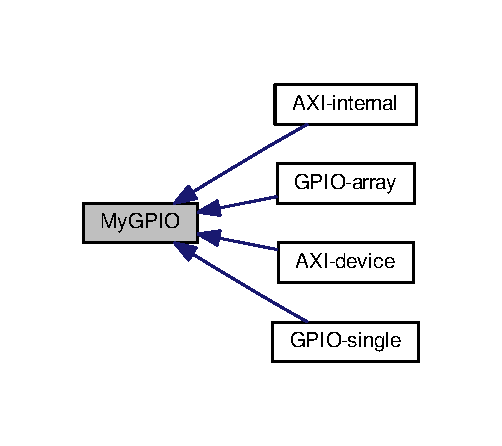
\includegraphics[width=240pt]{group__my_g_p_i_o}
\end{center}
\end{figure}
\subsection*{Moduli}
\begin{DoxyCompactItemize}
\item 
\hyperlink{group___linux-_driver}{Linux-\/\+Driver}
\end{DoxyCompactItemize}
\subsection*{Strutture dati}
\begin{DoxyCompactItemize}
\item 
struct \hyperlink{structmy_g_p_i_o__t}{my\+G\+P\+I\+O\+\_\+t}
\begin{DoxyCompactList}\small\item\em Struttura che astrae un device my\+G\+P\+I\+O. \end{DoxyCompactList}\end{DoxyCompactItemize}
\subsection*{Definizioni}
\begin{DoxyCompactItemize}
\item 
\#define \hyperlink{group__my_g_p_i_o_ga81a662103d6ed053978c0a9b4c273065}{my\+G\+P\+I\+O\+\_\+\+M\+O\+D\+E\+\_\+\+O\+F\+F\+S\+E\+T}~0\+U
\begin{DoxyCompactList}\small\item\em Offset, rispetto all'indirizzo base, del registro \char`\"{}mode\char`\"{} per il device my\+G\+P\+I\+O. \end{DoxyCompactList}\item 
\#define \hyperlink{group__my_g_p_i_o_ga2e45778b6ca9ce6f5768b3f7a4557ce1}{my\+G\+P\+I\+O\+\_\+\+W\+R\+I\+T\+E\+\_\+\+O\+F\+F\+S\+E\+T}~4\+U
\begin{DoxyCompactList}\small\item\em Offset, rispetto all'indirizzo base, del registro \char`\"{}write\char`\"{} per il device my\+G\+P\+I\+O. \end{DoxyCompactList}\item 
\#define \hyperlink{group__my_g_p_i_o_ga584d2dfece76e5762030d918d80592cc}{my\+G\+P\+I\+O\+\_\+\+R\+E\+A\+D\+\_\+\+O\+F\+F\+S\+E\+T}~8\+U
\begin{DoxyCompactList}\small\item\em Offset, rispetto all'indirizzo base, del registro \char`\"{}read\char`\"{} per il device my\+G\+P\+I\+O. \end{DoxyCompactList}\item 
\#define \hyperlink{group__my_g_p_i_o_gaacf2d8a21a051e778f02f8811b9c1e96}{my\+G\+P\+I\+O\+\_\+\+I\+N\+T\+R\+\_\+\+O\+F\+F\+S\+E\+T}~12\+U
\begin{DoxyCompactList}\small\item\em Offset, rispetto all'indirizzo base, del registro \char`\"{}interrupt\char`\"{} per il device my\+G\+P\+I\+O. \end{DoxyCompactList}\item 
\#define \hyperlink{group__my_g_p_i_o_ga0ba32e2adf874ed7216c5993369153e1}{my\+G\+P\+I\+O\+\_\+\+I\+N\+T\+R\+\_\+\+Int\+En\+\_\+mask}~0x1\+U
\begin{DoxyCompactList}\small\item\em maschera del bit del registro \char`\"{}interrupt\char`\"{} che funge da interrupt-\/enable, per il device my\+G\+P\+I\+O \end{DoxyCompactList}\item 
\#define \hyperlink{group__my_g_p_i_o_ga4cd02635783bc2a4ad7639cfb9fdb698}{my\+G\+P\+I\+O\+\_\+\+I\+N\+T\+R\+\_\+\+Irq\+\_\+mask}~0x2\+U
\begin{DoxyCompactList}\small\item\em maschera del bit del registro \char`\"{}interrupt\char`\"{} che funge da interrupt-\/request, per il device my\+G\+P\+I\+O \end{DoxyCompactList}\item 
\#define \hyperlink{group__my_g_p_i_o_gaa760b8397e6372e48c1008c2ba8d7387}{my\+G\+P\+I\+O\+\_\+\+I\+N\+T\+R\+\_\+\+Int\+Ack\+\_\+mask}~0x4\+U
\begin{DoxyCompactList}\small\item\em maschera del bit del registro \char`\"{}interrupt\char`\"{} che funge da interrupt-\/ack, per il device my\+G\+P\+I\+O \end{DoxyCompactList}\item 
\#define \hyperlink{group__my_g_p_i_o_gabbe2491a3b71c292521025b7b382b971}{my\+G\+P\+I\+O\+\_\+pin}(i)~((uint32\+\_\+t)(1$<$$<$(i)))
\begin{DoxyCompactList}\small\item\em Metodo alternativo per la specifica di uno dei pin di un device my\+G\+P\+I\+O. \end{DoxyCompactList}\end{DoxyCompactItemize}
\subsection*{Tipi enumerati (enum)}
\begin{DoxyCompactItemize}
\item 
enum \hyperlink{group__my_g_p_i_o_ga402a0d20afc0cb7c25554b8b023f4253}{my\+G\+P\+I\+O\+\_\+mask} \{ \\*
\hyperlink{group__my_g_p_i_o_gga402a0d20afc0cb7c25554b8b023f4253a6db6fa7be955ae379f543d96122e23a9}{my\+G\+P\+I\+O\+\_\+pin0} = 0x1\+U, 
\hyperlink{group__my_g_p_i_o_gga402a0d20afc0cb7c25554b8b023f4253a1de6bdcc01efca2c39f584f5a20293be}{my\+G\+P\+I\+O\+\_\+pin1} = 0x2\+U, 
\hyperlink{group__my_g_p_i_o_gga402a0d20afc0cb7c25554b8b023f4253a1fb3f52d920ac8ba17b74dd73c27d783}{my\+G\+P\+I\+O\+\_\+pin2} = 0x4\+U, 
\hyperlink{group__my_g_p_i_o_gga402a0d20afc0cb7c25554b8b023f4253a4514d64390392b626aa4dbfaac8dc1e5}{my\+G\+P\+I\+O\+\_\+pin3} = 0x8\+U, 
\\*
\hyperlink{group__my_g_p_i_o_gga402a0d20afc0cb7c25554b8b023f4253a0a446f53dee6f6f4ccb9a1d1f947b637}{my\+G\+P\+I\+O\+\_\+pin4} = 0x10\+U, 
\hyperlink{group__my_g_p_i_o_gga402a0d20afc0cb7c25554b8b023f4253a04a111036a27e9b97f0950f6d37b04d2}{my\+G\+P\+I\+O\+\_\+pin5} = 0x20\+U, 
\hyperlink{group__my_g_p_i_o_gga402a0d20afc0cb7c25554b8b023f4253a39a529f8c0a4f302029f54daa815471b}{my\+G\+P\+I\+O\+\_\+pin6} = 0x40\+U, 
\hyperlink{group__my_g_p_i_o_gga402a0d20afc0cb7c25554b8b023f4253af4e88b077442e4c0f459e1e4aa60626b}{my\+G\+P\+I\+O\+\_\+pin7} = 0x80\+U, 
\\*
\hyperlink{group__my_g_p_i_o_gga402a0d20afc0cb7c25554b8b023f4253a615159bcf4e347dc2b60f2545fae5f9e}{my\+G\+P\+I\+O\+\_\+pin8} = 0x100\+U, 
\hyperlink{group__my_g_p_i_o_gga402a0d20afc0cb7c25554b8b023f4253a8d721236fb936126a08c12b87696f6e9}{my\+G\+P\+I\+O\+\_\+pin9} = 0x200\+U, 
\hyperlink{group__my_g_p_i_o_gga402a0d20afc0cb7c25554b8b023f4253ae3067b7b3b1a2e171ecd74b6abd48341}{my\+G\+P\+I\+O\+\_\+pin10} = 0x400\+U, 
\hyperlink{group__my_g_p_i_o_gga402a0d20afc0cb7c25554b8b023f4253ae5c2e65508bfd452100d9da331d6220a}{my\+G\+P\+I\+O\+\_\+pin11} = 0x800\+U, 
\\*
\hyperlink{group__my_g_p_i_o_gga402a0d20afc0cb7c25554b8b023f4253afa75e3c1c019048c8553cb733c5137b5}{my\+G\+P\+I\+O\+\_\+pin12} = 0x1000\+U, 
\hyperlink{group__my_g_p_i_o_gga402a0d20afc0cb7c25554b8b023f4253a243381a796f0936a576f184dd115b37c}{my\+G\+P\+I\+O\+\_\+pin13} = 0x2000\+U, 
\hyperlink{group__my_g_p_i_o_gga402a0d20afc0cb7c25554b8b023f4253aed4915d6b3eab49cc1ba971b9f439fdd}{my\+G\+P\+I\+O\+\_\+pin14} = 0x4000\+U, 
\hyperlink{group__my_g_p_i_o_gga402a0d20afc0cb7c25554b8b023f4253a46c427ea97182a77e8c975d3429a64ee}{my\+G\+P\+I\+O\+\_\+pin15} = 0x8000\+U, 
\\*
\hyperlink{group__my_g_p_i_o_gga402a0d20afc0cb7c25554b8b023f4253a5a27c4d87207b2eba865876854f1ba67}{my\+G\+P\+I\+O\+\_\+pin16} = 0x10000\+U, 
\hyperlink{group__my_g_p_i_o_gga402a0d20afc0cb7c25554b8b023f4253ab0541af31059bdc8dca44d5dafa7e779}{my\+G\+P\+I\+O\+\_\+pin17} = 0x20000\+U, 
\hyperlink{group__my_g_p_i_o_gga402a0d20afc0cb7c25554b8b023f4253a7a51a492e3cb580581a2c8eb439edd99}{my\+G\+P\+I\+O\+\_\+pin18} = 0x40000\+U, 
\hyperlink{group__my_g_p_i_o_gga402a0d20afc0cb7c25554b8b023f4253a9118ae2775e93bd4522660e81a2d5309}{my\+G\+P\+I\+O\+\_\+pin19} = 0x80000\+U, 
\\*
\hyperlink{group__my_g_p_i_o_gga402a0d20afc0cb7c25554b8b023f4253a7940782a16f88dbbb3a4037c2bef1711}{my\+G\+P\+I\+O\+\_\+pin20} = 0x100000\+U, 
\hyperlink{group__my_g_p_i_o_gga402a0d20afc0cb7c25554b8b023f4253a1da616a8cf4396927db1e5a336fb6dc5}{my\+G\+P\+I\+O\+\_\+pin21} = 0x200000\+U, 
\hyperlink{group__my_g_p_i_o_gga402a0d20afc0cb7c25554b8b023f4253acf80113da8d789f7da9f9edc4ab6003c}{my\+G\+P\+I\+O\+\_\+pin22} = 0x400000\+U, 
\hyperlink{group__my_g_p_i_o_gga402a0d20afc0cb7c25554b8b023f4253ad64e03b703608de173ab5950b5121830}{my\+G\+P\+I\+O\+\_\+pin23} = 0x800000\+U, 
\\*
\hyperlink{group__my_g_p_i_o_gga402a0d20afc0cb7c25554b8b023f4253a5bb93f546327123f81b06ed0dfcdf110}{my\+G\+P\+I\+O\+\_\+pin24} = 0x1000000\+U, 
\hyperlink{group__my_g_p_i_o_gga402a0d20afc0cb7c25554b8b023f4253a0b27a7e78aff5836f33085f3b4539f56}{my\+G\+P\+I\+O\+\_\+pin25} = 0x2000000\+U, 
\hyperlink{group__my_g_p_i_o_gga402a0d20afc0cb7c25554b8b023f4253aaa07c24140250dcbc695206793efa8af}{my\+G\+P\+I\+O\+\_\+pin26} = 0x4000000\+U, 
\hyperlink{group__my_g_p_i_o_gga402a0d20afc0cb7c25554b8b023f4253a1dd5e99eba6237aeb30b2194c553c37f}{my\+G\+P\+I\+O\+\_\+pin27} = 0x8000000\+U, 
\\*
\hyperlink{group__my_g_p_i_o_gga402a0d20afc0cb7c25554b8b023f4253a2076590efec8bcf9ef3285798753e632}{my\+G\+P\+I\+O\+\_\+pin28} = 0x10000000\+U, 
\hyperlink{group__my_g_p_i_o_gga402a0d20afc0cb7c25554b8b023f4253abfe9540fa3946a35e20f7f68cb1b8084}{my\+G\+P\+I\+O\+\_\+pin29} = 0x20000000\+U, 
\hyperlink{group__my_g_p_i_o_gga402a0d20afc0cb7c25554b8b023f4253a59993a30c537c116eddb42d10778f4f8}{my\+G\+P\+I\+O\+\_\+pin30} = 0x40000000\+U, 
\hyperlink{group__my_g_p_i_o_gga402a0d20afc0cb7c25554b8b023f4253a9a55b7c245bd9aad750b7891d27e9225}{my\+G\+P\+I\+O\+\_\+pin31} = 0x80000000\+U, 
\\*
\hyperlink{group__my_g_p_i_o_gga402a0d20afc0cb7c25554b8b023f4253a0347b1742eef6b2575a7d409c7fb5c3d}{my\+G\+P\+I\+O\+\_\+byte0} = 0x000000ff\+U, 
\hyperlink{group__my_g_p_i_o_gga402a0d20afc0cb7c25554b8b023f4253ae5aec65fa20f554b893e419fc2755fd0}{my\+G\+P\+I\+O\+\_\+byte1} = 0x0000ff00\+U, 
\hyperlink{group__my_g_p_i_o_gga402a0d20afc0cb7c25554b8b023f4253af4892f7db28c64a7cf2a7236c88b742b}{my\+G\+P\+I\+O\+\_\+byte2} = 0x00ff0000\+U, 
\hyperlink{group__my_g_p_i_o_gga402a0d20afc0cb7c25554b8b023f4253a1ceefb9d65397352e986c573984d0129}{my\+G\+P\+I\+O\+\_\+byte3} = 0xff000000\+U
 \}
\begin{DoxyCompactList}\small\item\em Maschere di selezione dei pin di un device my\+G\+P\+I\+O. \end{DoxyCompactList}\item 
enum \hyperlink{group__my_g_p_i_o_ga76b849f0e0c05e7f9161bdb33396f2b1}{my\+G\+P\+I\+O\+\_\+mode} \{ \hyperlink{group__my_g_p_i_o_gga76b849f0e0c05e7f9161bdb33396f2b1a1e6dc78e7641e878cadc842d39605d5d}{my\+G\+P\+I\+O\+\_\+read}, 
\hyperlink{group__my_g_p_i_o_gga76b849f0e0c05e7f9161bdb33396f2b1a2d66976280eb7595a42c631683bdfad6}{my\+G\+P\+I\+O\+\_\+write}
 \}
\begin{DoxyCompactList}\small\item\em my\+G\+P\+I\+O\+\_\+mode, modalita' di funzionamento (lettura/scrittura) di un device my\+G\+P\+I\+O \end{DoxyCompactList}\item 
enum \hyperlink{group__my_g_p_i_o_gaf634fe4a0e1eab8da5000b72d6ad362b}{my\+G\+P\+I\+O\+\_\+value} \{ \hyperlink{group__my_g_p_i_o_ggaf634fe4a0e1eab8da5000b72d6ad362ba98cde80dbda025bd1ae7231c76b55674}{my\+G\+P\+I\+O\+\_\+reset}, 
\hyperlink{group__my_g_p_i_o_ggaf634fe4a0e1eab8da5000b72d6ad362ba10d296f3711d01189cc6c2d87f7c9149}{my\+G\+P\+I\+O\+\_\+set}
 \}
\begin{DoxyCompactList}\small\item\em my\+G\+P\+I\+O\+\_\+value, valore di un my\+G\+P\+I\+O \end{DoxyCompactList}\end{DoxyCompactItemize}
\subsection*{Funzioni}
\begin{DoxyCompactItemize}
\item 
void \hyperlink{group__my_g_p_i_o_ga8fda7ca73b187baf256409423c25d725}{my\+G\+P\+I\+O\+\_\+init} (\hyperlink{structmy_g_p_i_o__t}{my\+G\+P\+I\+O\+\_\+t} $\ast$gpio, uint32\+\_\+t base\+\_\+address)
\begin{DoxyCompactList}\small\item\em Inizializza un device my\+G\+P\+I\+O. \end{DoxyCompactList}\item 
void \hyperlink{group__my_g_p_i_o_ga38a2ea04d07af50f7f570f0367594c8b}{my\+G\+P\+I\+O\+\_\+set\+Mode} (\hyperlink{structmy_g_p_i_o__t}{my\+G\+P\+I\+O\+\_\+t} $\ast$gpio, \hyperlink{group__my_g_p_i_o_ga402a0d20afc0cb7c25554b8b023f4253}{my\+G\+P\+I\+O\+\_\+mask} mask, \hyperlink{group__my_g_p_i_o_ga76b849f0e0c05e7f9161bdb33396f2b1}{my\+G\+P\+I\+O\+\_\+mode} mode)
\begin{DoxyCompactList}\small\item\em Permette di settare la modalita' lettura/scrittura dei pin di un device my\+G\+P\+I\+O;. \end{DoxyCompactList}\item 
void \hyperlink{group__my_g_p_i_o_gab742e68093ad4c90fe299b64fd6736ca}{my\+G\+P\+I\+O\+\_\+set\+Value} (\hyperlink{structmy_g_p_i_o__t}{my\+G\+P\+I\+O\+\_\+t} $\ast$gpio, \hyperlink{group__my_g_p_i_o_ga402a0d20afc0cb7c25554b8b023f4253}{my\+G\+P\+I\+O\+\_\+mask} mask, \hyperlink{group__my_g_p_i_o_gaf634fe4a0e1eab8da5000b72d6ad362b}{my\+G\+P\+I\+O\+\_\+value} value)
\begin{DoxyCompactList}\small\item\em Permette di settare il valore dei pin di un device my\+G\+P\+I\+O, se configurati come output. \end{DoxyCompactList}\item 
void \hyperlink{group__my_g_p_i_o_ga27ea411bf51a58fe48eb8c5036780b53}{my\+G\+P\+I\+O\+\_\+toggle} (\hyperlink{structmy_g_p_i_o__t}{my\+G\+P\+I\+O\+\_\+t} $\ast$gpio, \hyperlink{group__my_g_p_i_o_ga402a0d20afc0cb7c25554b8b023f4253}{my\+G\+P\+I\+O\+\_\+mask} mask)
\begin{DoxyCompactList}\small\item\em Permette di invertire il valore dei pin di un device my\+G\+P\+I\+O, se configurati come output. \end{DoxyCompactList}\item 
\hyperlink{group__my_g_p_i_o_gaf634fe4a0e1eab8da5000b72d6ad362b}{my\+G\+P\+I\+O\+\_\+value} \hyperlink{group__my_g_p_i_o_gad6576f1d0fb17d9b492da0b1008550d0}{my\+G\+P\+I\+O\+\_\+get\+Value} (\hyperlink{structmy_g_p_i_o__t}{my\+G\+P\+I\+O\+\_\+t} $\ast$gpio, \hyperlink{group__my_g_p_i_o_ga402a0d20afc0cb7c25554b8b023f4253}{my\+G\+P\+I\+O\+\_\+mask} mask)
\begin{DoxyCompactList}\small\item\em Permette di leggere il valore dei pin di un device my\+G\+P\+I\+O;. \end{DoxyCompactList}\item 
\hyperlink{group__my_g_p_i_o_ga402a0d20afc0cb7c25554b8b023f4253}{my\+G\+P\+I\+O\+\_\+mask} \hyperlink{group__my_g_p_i_o_gadb3ecd03ea82420488977134c9313e18}{my\+G\+P\+I\+O\+\_\+get\+Read} (\hyperlink{structmy_g_p_i_o__t}{my\+G\+P\+I\+O\+\_\+t} $\ast$gpio)
\begin{DoxyCompactList}\small\item\em Restituisce la maschera dei pin settati di un device my\+G\+P\+I\+O. \end{DoxyCompactList}\item 
void \hyperlink{group__my_g_p_i_o_ga39822bfa495a9388e81ced74884c06a2}{my\+G\+P\+I\+O\+\_\+interrupt\+Enable} (\hyperlink{structmy_g_p_i_o__t}{my\+G\+P\+I\+O\+\_\+t} $\ast$gpio)
\begin{DoxyCompactList}\small\item\em Abilita gli interrupt per un device my\+G\+P\+I\+O. \end{DoxyCompactList}\item 
void \hyperlink{group__my_g_p_i_o_gab681db0119860bfad2c3e674289d8b3d}{my\+G\+P\+I\+O\+\_\+interrupt\+Disable} (\hyperlink{structmy_g_p_i_o__t}{my\+G\+P\+I\+O\+\_\+t} $\ast$gpio)
\begin{DoxyCompactList}\small\item\em Disabilita gli interrupt per un device my\+G\+P\+I\+O. \end{DoxyCompactList}\item 
void \hyperlink{group__my_g_p_i_o_ga396f6e5e7f0eeff01e98fcc78523402b}{my\+G\+P\+I\+O\+\_\+interrupt\+Ack} (\hyperlink{structmy_g_p_i_o__t}{my\+G\+P\+I\+O\+\_\+t} $\ast$gpio)
\begin{DoxyCompactList}\small\item\em Segnala al device che l'interruzione da lui sollevata e' stata servita. \end{DoxyCompactList}\item 
\hyperlink{group__my_g_p_i_o_gaf634fe4a0e1eab8da5000b72d6ad362b}{my\+G\+P\+I\+O\+\_\+value} \hyperlink{group__my_g_p_i_o_ga7936b506b45f116de68ddf06c84cc242}{my\+G\+P\+I\+O\+\_\+get\+Irq} (\hyperlink{structmy_g_p_i_o__t}{my\+G\+P\+I\+O\+\_\+t} $\ast$gpio)
\begin{DoxyCompactList}\small\item\em Consente di verificare se un device my\+G\+P\+I\+O abbia generato un'interruzione. \end{DoxyCompactList}\end{DoxyCompactItemize}


\subsection{Descrizione dettagliata}
Il modulo definisce un driver O\+O-\/like per l'utilizzo di una periferica my\+G\+P\+I\+O custom. 

\subsection{Documentazione delle definizioni}
\hypertarget{group__my_g_p_i_o_gaa760b8397e6372e48c1008c2ba8d7387}{\index{My\+G\+P\+I\+O@{My\+G\+P\+I\+O}!my\+G\+P\+I\+O\+\_\+\+I\+N\+T\+R\+\_\+\+Int\+Ack\+\_\+mask@{my\+G\+P\+I\+O\+\_\+\+I\+N\+T\+R\+\_\+\+Int\+Ack\+\_\+mask}}
\index{my\+G\+P\+I\+O\+\_\+\+I\+N\+T\+R\+\_\+\+Int\+Ack\+\_\+mask@{my\+G\+P\+I\+O\+\_\+\+I\+N\+T\+R\+\_\+\+Int\+Ack\+\_\+mask}!My\+G\+P\+I\+O@{My\+G\+P\+I\+O}}
\subsubsection[{my\+G\+P\+I\+O\+\_\+\+I\+N\+T\+R\+\_\+\+Int\+Ack\+\_\+mask}]{\setlength{\rightskip}{0pt plus 5cm}\#define my\+G\+P\+I\+O\+\_\+\+I\+N\+T\+R\+\_\+\+Int\+Ack\+\_\+mask~0x4\+U}}\label{group__my_g_p_i_o_gaa760b8397e6372e48c1008c2ba8d7387}


maschera del bit del registro \char`\"{}interrupt\char`\"{} che funge da interrupt-\/ack, per il device my\+G\+P\+I\+O 

\hypertarget{group__my_g_p_i_o_ga0ba32e2adf874ed7216c5993369153e1}{\index{My\+G\+P\+I\+O@{My\+G\+P\+I\+O}!my\+G\+P\+I\+O\+\_\+\+I\+N\+T\+R\+\_\+\+Int\+En\+\_\+mask@{my\+G\+P\+I\+O\+\_\+\+I\+N\+T\+R\+\_\+\+Int\+En\+\_\+mask}}
\index{my\+G\+P\+I\+O\+\_\+\+I\+N\+T\+R\+\_\+\+Int\+En\+\_\+mask@{my\+G\+P\+I\+O\+\_\+\+I\+N\+T\+R\+\_\+\+Int\+En\+\_\+mask}!My\+G\+P\+I\+O@{My\+G\+P\+I\+O}}
\subsubsection[{my\+G\+P\+I\+O\+\_\+\+I\+N\+T\+R\+\_\+\+Int\+En\+\_\+mask}]{\setlength{\rightskip}{0pt plus 5cm}\#define my\+G\+P\+I\+O\+\_\+\+I\+N\+T\+R\+\_\+\+Int\+En\+\_\+mask~0x1\+U}}\label{group__my_g_p_i_o_ga0ba32e2adf874ed7216c5993369153e1}


maschera del bit del registro \char`\"{}interrupt\char`\"{} che funge da interrupt-\/enable, per il device my\+G\+P\+I\+O 

\hypertarget{group__my_g_p_i_o_ga4cd02635783bc2a4ad7639cfb9fdb698}{\index{My\+G\+P\+I\+O@{My\+G\+P\+I\+O}!my\+G\+P\+I\+O\+\_\+\+I\+N\+T\+R\+\_\+\+Irq\+\_\+mask@{my\+G\+P\+I\+O\+\_\+\+I\+N\+T\+R\+\_\+\+Irq\+\_\+mask}}
\index{my\+G\+P\+I\+O\+\_\+\+I\+N\+T\+R\+\_\+\+Irq\+\_\+mask@{my\+G\+P\+I\+O\+\_\+\+I\+N\+T\+R\+\_\+\+Irq\+\_\+mask}!My\+G\+P\+I\+O@{My\+G\+P\+I\+O}}
\subsubsection[{my\+G\+P\+I\+O\+\_\+\+I\+N\+T\+R\+\_\+\+Irq\+\_\+mask}]{\setlength{\rightskip}{0pt plus 5cm}\#define my\+G\+P\+I\+O\+\_\+\+I\+N\+T\+R\+\_\+\+Irq\+\_\+mask~0x2\+U}}\label{group__my_g_p_i_o_ga4cd02635783bc2a4ad7639cfb9fdb698}


maschera del bit del registro \char`\"{}interrupt\char`\"{} che funge da interrupt-\/request, per il device my\+G\+P\+I\+O 

\hypertarget{group__my_g_p_i_o_gaacf2d8a21a051e778f02f8811b9c1e96}{\index{My\+G\+P\+I\+O@{My\+G\+P\+I\+O}!my\+G\+P\+I\+O\+\_\+\+I\+N\+T\+R\+\_\+\+O\+F\+F\+S\+E\+T@{my\+G\+P\+I\+O\+\_\+\+I\+N\+T\+R\+\_\+\+O\+F\+F\+S\+E\+T}}
\index{my\+G\+P\+I\+O\+\_\+\+I\+N\+T\+R\+\_\+\+O\+F\+F\+S\+E\+T@{my\+G\+P\+I\+O\+\_\+\+I\+N\+T\+R\+\_\+\+O\+F\+F\+S\+E\+T}!My\+G\+P\+I\+O@{My\+G\+P\+I\+O}}
\subsubsection[{my\+G\+P\+I\+O\+\_\+\+I\+N\+T\+R\+\_\+\+O\+F\+F\+S\+E\+T}]{\setlength{\rightskip}{0pt plus 5cm}\#define my\+G\+P\+I\+O\+\_\+\+I\+N\+T\+R\+\_\+\+O\+F\+F\+S\+E\+T~12\+U}}\label{group__my_g_p_i_o_gaacf2d8a21a051e778f02f8811b9c1e96}


Offset, rispetto all'indirizzo base, del registro \char`\"{}interrupt\char`\"{} per il device my\+G\+P\+I\+O. 

\hypertarget{group__my_g_p_i_o_ga81a662103d6ed053978c0a9b4c273065}{\index{My\+G\+P\+I\+O@{My\+G\+P\+I\+O}!my\+G\+P\+I\+O\+\_\+\+M\+O\+D\+E\+\_\+\+O\+F\+F\+S\+E\+T@{my\+G\+P\+I\+O\+\_\+\+M\+O\+D\+E\+\_\+\+O\+F\+F\+S\+E\+T}}
\index{my\+G\+P\+I\+O\+\_\+\+M\+O\+D\+E\+\_\+\+O\+F\+F\+S\+E\+T@{my\+G\+P\+I\+O\+\_\+\+M\+O\+D\+E\+\_\+\+O\+F\+F\+S\+E\+T}!My\+G\+P\+I\+O@{My\+G\+P\+I\+O}}
\subsubsection[{my\+G\+P\+I\+O\+\_\+\+M\+O\+D\+E\+\_\+\+O\+F\+F\+S\+E\+T}]{\setlength{\rightskip}{0pt plus 5cm}\#define my\+G\+P\+I\+O\+\_\+\+M\+O\+D\+E\+\_\+\+O\+F\+F\+S\+E\+T~0\+U}}\label{group__my_g_p_i_o_ga81a662103d6ed053978c0a9b4c273065}


Offset, rispetto all'indirizzo base, del registro \char`\"{}mode\char`\"{} per il device my\+G\+P\+I\+O. 

\hypertarget{group__my_g_p_i_o_gabbe2491a3b71c292521025b7b382b971}{\index{My\+G\+P\+I\+O@{My\+G\+P\+I\+O}!my\+G\+P\+I\+O\+\_\+pin@{my\+G\+P\+I\+O\+\_\+pin}}
\index{my\+G\+P\+I\+O\+\_\+pin@{my\+G\+P\+I\+O\+\_\+pin}!My\+G\+P\+I\+O@{My\+G\+P\+I\+O}}
\subsubsection[{my\+G\+P\+I\+O\+\_\+pin}]{\setlength{\rightskip}{0pt plus 5cm}\#define my\+G\+P\+I\+O\+\_\+pin(
\begin{DoxyParamCaption}
\item[{}]{i}
\end{DoxyParamCaption}
)~((uint32\+\_\+t)(1$<$$<$(i)))}}\label{group__my_g_p_i_o_gabbe2491a3b71c292521025b7b382b971}


Metodo alternativo per la specifica di uno dei pin di un device my\+G\+P\+I\+O. 


\begin{DoxyParams}[1]{Parametri}
\mbox{\tt in}  & {\em i} & indice del bit da selezionare, da 0 (bit meno significativo) a 31 (bit piu' significativo) \\
\hline
\end{DoxyParams}
\begin{DoxyReturn}{Restituisce}
maschera di selezione del pin i-\/esimo 
\end{DoxyReturn}
\hypertarget{group__my_g_p_i_o_ga584d2dfece76e5762030d918d80592cc}{\index{My\+G\+P\+I\+O@{My\+G\+P\+I\+O}!my\+G\+P\+I\+O\+\_\+\+R\+E\+A\+D\+\_\+\+O\+F\+F\+S\+E\+T@{my\+G\+P\+I\+O\+\_\+\+R\+E\+A\+D\+\_\+\+O\+F\+F\+S\+E\+T}}
\index{my\+G\+P\+I\+O\+\_\+\+R\+E\+A\+D\+\_\+\+O\+F\+F\+S\+E\+T@{my\+G\+P\+I\+O\+\_\+\+R\+E\+A\+D\+\_\+\+O\+F\+F\+S\+E\+T}!My\+G\+P\+I\+O@{My\+G\+P\+I\+O}}
\subsubsection[{my\+G\+P\+I\+O\+\_\+\+R\+E\+A\+D\+\_\+\+O\+F\+F\+S\+E\+T}]{\setlength{\rightskip}{0pt plus 5cm}\#define my\+G\+P\+I\+O\+\_\+\+R\+E\+A\+D\+\_\+\+O\+F\+F\+S\+E\+T~8\+U}}\label{group__my_g_p_i_o_ga584d2dfece76e5762030d918d80592cc}


Offset, rispetto all'indirizzo base, del registro \char`\"{}read\char`\"{} per il device my\+G\+P\+I\+O. 

\hypertarget{group__my_g_p_i_o_ga2e45778b6ca9ce6f5768b3f7a4557ce1}{\index{My\+G\+P\+I\+O@{My\+G\+P\+I\+O}!my\+G\+P\+I\+O\+\_\+\+W\+R\+I\+T\+E\+\_\+\+O\+F\+F\+S\+E\+T@{my\+G\+P\+I\+O\+\_\+\+W\+R\+I\+T\+E\+\_\+\+O\+F\+F\+S\+E\+T}}
\index{my\+G\+P\+I\+O\+\_\+\+W\+R\+I\+T\+E\+\_\+\+O\+F\+F\+S\+E\+T@{my\+G\+P\+I\+O\+\_\+\+W\+R\+I\+T\+E\+\_\+\+O\+F\+F\+S\+E\+T}!My\+G\+P\+I\+O@{My\+G\+P\+I\+O}}
\subsubsection[{my\+G\+P\+I\+O\+\_\+\+W\+R\+I\+T\+E\+\_\+\+O\+F\+F\+S\+E\+T}]{\setlength{\rightskip}{0pt plus 5cm}\#define my\+G\+P\+I\+O\+\_\+\+W\+R\+I\+T\+E\+\_\+\+O\+F\+F\+S\+E\+T~4\+U}}\label{group__my_g_p_i_o_ga2e45778b6ca9ce6f5768b3f7a4557ce1}


Offset, rispetto all'indirizzo base, del registro \char`\"{}write\char`\"{} per il device my\+G\+P\+I\+O. 



\subsection{Documentazione dei tipi enumerati}
\hypertarget{group__my_g_p_i_o_ga402a0d20afc0cb7c25554b8b023f4253}{\index{My\+G\+P\+I\+O@{My\+G\+P\+I\+O}!my\+G\+P\+I\+O\+\_\+mask@{my\+G\+P\+I\+O\+\_\+mask}}
\index{my\+G\+P\+I\+O\+\_\+mask@{my\+G\+P\+I\+O\+\_\+mask}!My\+G\+P\+I\+O@{My\+G\+P\+I\+O}}
\subsubsection[{my\+G\+P\+I\+O\+\_\+mask}]{\setlength{\rightskip}{0pt plus 5cm}enum {\bf my\+G\+P\+I\+O\+\_\+mask}}}\label{group__my_g_p_i_o_ga402a0d20afc0cb7c25554b8b023f4253}


Maschere di selezione dei pin di un device my\+G\+P\+I\+O. 

\begin{Desc}
\item[Valori del tipo enumerato]\par
\begin{description}
\index{my\+G\+P\+I\+O\+\_\+pin0@{my\+G\+P\+I\+O\+\_\+pin0}!My\+G\+P\+I\+O@{My\+G\+P\+I\+O}}\index{My\+G\+P\+I\+O@{My\+G\+P\+I\+O}!my\+G\+P\+I\+O\+\_\+pin0@{my\+G\+P\+I\+O\+\_\+pin0}}\item[{\em 
\hypertarget{group__my_g_p_i_o_gga402a0d20afc0cb7c25554b8b023f4253a6db6fa7be955ae379f543d96122e23a9}{my\+G\+P\+I\+O\+\_\+pin0}\label{group__my_g_p_i_o_gga402a0d20afc0cb7c25554b8b023f4253a6db6fa7be955ae379f543d96122e23a9}
}]my\+G\+P\+I\+O pin0 maschera di selezione del pin 0 di un device my\+G\+P\+I\+O \index{my\+G\+P\+I\+O\+\_\+pin1@{my\+G\+P\+I\+O\+\_\+pin1}!My\+G\+P\+I\+O@{My\+G\+P\+I\+O}}\index{My\+G\+P\+I\+O@{My\+G\+P\+I\+O}!my\+G\+P\+I\+O\+\_\+pin1@{my\+G\+P\+I\+O\+\_\+pin1}}\item[{\em 
\hypertarget{group__my_g_p_i_o_gga402a0d20afc0cb7c25554b8b023f4253a1de6bdcc01efca2c39f584f5a20293be}{my\+G\+P\+I\+O\+\_\+pin1}\label{group__my_g_p_i_o_gga402a0d20afc0cb7c25554b8b023f4253a1de6bdcc01efca2c39f584f5a20293be}
}]my\+G\+P\+I\+O pin1 maschera di selezione del pin 1 di un device my\+G\+P\+I\+O \index{my\+G\+P\+I\+O\+\_\+pin2@{my\+G\+P\+I\+O\+\_\+pin2}!My\+G\+P\+I\+O@{My\+G\+P\+I\+O}}\index{My\+G\+P\+I\+O@{My\+G\+P\+I\+O}!my\+G\+P\+I\+O\+\_\+pin2@{my\+G\+P\+I\+O\+\_\+pin2}}\item[{\em 
\hypertarget{group__my_g_p_i_o_gga402a0d20afc0cb7c25554b8b023f4253a1fb3f52d920ac8ba17b74dd73c27d783}{my\+G\+P\+I\+O\+\_\+pin2}\label{group__my_g_p_i_o_gga402a0d20afc0cb7c25554b8b023f4253a1fb3f52d920ac8ba17b74dd73c27d783}
}]my\+G\+P\+I\+O pin2 maschera di selezione del pin 2 di un device my\+G\+P\+I\+O \index{my\+G\+P\+I\+O\+\_\+pin3@{my\+G\+P\+I\+O\+\_\+pin3}!My\+G\+P\+I\+O@{My\+G\+P\+I\+O}}\index{My\+G\+P\+I\+O@{My\+G\+P\+I\+O}!my\+G\+P\+I\+O\+\_\+pin3@{my\+G\+P\+I\+O\+\_\+pin3}}\item[{\em 
\hypertarget{group__my_g_p_i_o_gga402a0d20afc0cb7c25554b8b023f4253a4514d64390392b626aa4dbfaac8dc1e5}{my\+G\+P\+I\+O\+\_\+pin3}\label{group__my_g_p_i_o_gga402a0d20afc0cb7c25554b8b023f4253a4514d64390392b626aa4dbfaac8dc1e5}
}]my\+G\+P\+I\+O pin3 maschera di selezione del pin 3 di un device my\+G\+P\+I\+O \index{my\+G\+P\+I\+O\+\_\+pin4@{my\+G\+P\+I\+O\+\_\+pin4}!My\+G\+P\+I\+O@{My\+G\+P\+I\+O}}\index{My\+G\+P\+I\+O@{My\+G\+P\+I\+O}!my\+G\+P\+I\+O\+\_\+pin4@{my\+G\+P\+I\+O\+\_\+pin4}}\item[{\em 
\hypertarget{group__my_g_p_i_o_gga402a0d20afc0cb7c25554b8b023f4253a0a446f53dee6f6f4ccb9a1d1f947b637}{my\+G\+P\+I\+O\+\_\+pin4}\label{group__my_g_p_i_o_gga402a0d20afc0cb7c25554b8b023f4253a0a446f53dee6f6f4ccb9a1d1f947b637}
}]my\+G\+P\+I\+O pin4 maschera di selezione del pin 4 di un device my\+G\+P\+I\+O \index{my\+G\+P\+I\+O\+\_\+pin5@{my\+G\+P\+I\+O\+\_\+pin5}!My\+G\+P\+I\+O@{My\+G\+P\+I\+O}}\index{My\+G\+P\+I\+O@{My\+G\+P\+I\+O}!my\+G\+P\+I\+O\+\_\+pin5@{my\+G\+P\+I\+O\+\_\+pin5}}\item[{\em 
\hypertarget{group__my_g_p_i_o_gga402a0d20afc0cb7c25554b8b023f4253a04a111036a27e9b97f0950f6d37b04d2}{my\+G\+P\+I\+O\+\_\+pin5}\label{group__my_g_p_i_o_gga402a0d20afc0cb7c25554b8b023f4253a04a111036a27e9b97f0950f6d37b04d2}
}]my\+G\+P\+I\+O pin5 maschera di selezione del pin 5 di un device my\+G\+P\+I\+O \index{my\+G\+P\+I\+O\+\_\+pin6@{my\+G\+P\+I\+O\+\_\+pin6}!My\+G\+P\+I\+O@{My\+G\+P\+I\+O}}\index{My\+G\+P\+I\+O@{My\+G\+P\+I\+O}!my\+G\+P\+I\+O\+\_\+pin6@{my\+G\+P\+I\+O\+\_\+pin6}}\item[{\em 
\hypertarget{group__my_g_p_i_o_gga402a0d20afc0cb7c25554b8b023f4253a39a529f8c0a4f302029f54daa815471b}{my\+G\+P\+I\+O\+\_\+pin6}\label{group__my_g_p_i_o_gga402a0d20afc0cb7c25554b8b023f4253a39a529f8c0a4f302029f54daa815471b}
}]my\+G\+P\+I\+O pin6 maschera di selezione del pin 6 di un device my\+G\+P\+I\+O \index{my\+G\+P\+I\+O\+\_\+pin7@{my\+G\+P\+I\+O\+\_\+pin7}!My\+G\+P\+I\+O@{My\+G\+P\+I\+O}}\index{My\+G\+P\+I\+O@{My\+G\+P\+I\+O}!my\+G\+P\+I\+O\+\_\+pin7@{my\+G\+P\+I\+O\+\_\+pin7}}\item[{\em 
\hypertarget{group__my_g_p_i_o_gga402a0d20afc0cb7c25554b8b023f4253af4e88b077442e4c0f459e1e4aa60626b}{my\+G\+P\+I\+O\+\_\+pin7}\label{group__my_g_p_i_o_gga402a0d20afc0cb7c25554b8b023f4253af4e88b077442e4c0f459e1e4aa60626b}
}]my\+G\+P\+I\+O pin7 maschera di selezione del pin 7 di un device my\+G\+P\+I\+O \index{my\+G\+P\+I\+O\+\_\+pin8@{my\+G\+P\+I\+O\+\_\+pin8}!My\+G\+P\+I\+O@{My\+G\+P\+I\+O}}\index{My\+G\+P\+I\+O@{My\+G\+P\+I\+O}!my\+G\+P\+I\+O\+\_\+pin8@{my\+G\+P\+I\+O\+\_\+pin8}}\item[{\em 
\hypertarget{group__my_g_p_i_o_gga402a0d20afc0cb7c25554b8b023f4253a615159bcf4e347dc2b60f2545fae5f9e}{my\+G\+P\+I\+O\+\_\+pin8}\label{group__my_g_p_i_o_gga402a0d20afc0cb7c25554b8b023f4253a615159bcf4e347dc2b60f2545fae5f9e}
}]my\+G\+P\+I\+O pin8 maschera di selezione del pin 8 di un device my\+G\+P\+I\+O \index{my\+G\+P\+I\+O\+\_\+pin9@{my\+G\+P\+I\+O\+\_\+pin9}!My\+G\+P\+I\+O@{My\+G\+P\+I\+O}}\index{My\+G\+P\+I\+O@{My\+G\+P\+I\+O}!my\+G\+P\+I\+O\+\_\+pin9@{my\+G\+P\+I\+O\+\_\+pin9}}\item[{\em 
\hypertarget{group__my_g_p_i_o_gga402a0d20afc0cb7c25554b8b023f4253a8d721236fb936126a08c12b87696f6e9}{my\+G\+P\+I\+O\+\_\+pin9}\label{group__my_g_p_i_o_gga402a0d20afc0cb7c25554b8b023f4253a8d721236fb936126a08c12b87696f6e9}
}]my\+G\+P\+I\+O pin9 maschera di selezione del pin 9 di un device my\+G\+P\+I\+O \index{my\+G\+P\+I\+O\+\_\+pin10@{my\+G\+P\+I\+O\+\_\+pin10}!My\+G\+P\+I\+O@{My\+G\+P\+I\+O}}\index{My\+G\+P\+I\+O@{My\+G\+P\+I\+O}!my\+G\+P\+I\+O\+\_\+pin10@{my\+G\+P\+I\+O\+\_\+pin10}}\item[{\em 
\hypertarget{group__my_g_p_i_o_gga402a0d20afc0cb7c25554b8b023f4253ae3067b7b3b1a2e171ecd74b6abd48341}{my\+G\+P\+I\+O\+\_\+pin10}\label{group__my_g_p_i_o_gga402a0d20afc0cb7c25554b8b023f4253ae3067b7b3b1a2e171ecd74b6abd48341}
}]my\+G\+P\+I\+O pin10 maschera di selezione del pin 10 di un device my\+G\+P\+I\+O \index{my\+G\+P\+I\+O\+\_\+pin11@{my\+G\+P\+I\+O\+\_\+pin11}!My\+G\+P\+I\+O@{My\+G\+P\+I\+O}}\index{My\+G\+P\+I\+O@{My\+G\+P\+I\+O}!my\+G\+P\+I\+O\+\_\+pin11@{my\+G\+P\+I\+O\+\_\+pin11}}\item[{\em 
\hypertarget{group__my_g_p_i_o_gga402a0d20afc0cb7c25554b8b023f4253ae5c2e65508bfd452100d9da331d6220a}{my\+G\+P\+I\+O\+\_\+pin11}\label{group__my_g_p_i_o_gga402a0d20afc0cb7c25554b8b023f4253ae5c2e65508bfd452100d9da331d6220a}
}]my\+G\+P\+I\+O pin11 maschera di selezione del pin 11 di un device my\+G\+P\+I\+O \index{my\+G\+P\+I\+O\+\_\+pin12@{my\+G\+P\+I\+O\+\_\+pin12}!My\+G\+P\+I\+O@{My\+G\+P\+I\+O}}\index{My\+G\+P\+I\+O@{My\+G\+P\+I\+O}!my\+G\+P\+I\+O\+\_\+pin12@{my\+G\+P\+I\+O\+\_\+pin12}}\item[{\em 
\hypertarget{group__my_g_p_i_o_gga402a0d20afc0cb7c25554b8b023f4253afa75e3c1c019048c8553cb733c5137b5}{my\+G\+P\+I\+O\+\_\+pin12}\label{group__my_g_p_i_o_gga402a0d20afc0cb7c25554b8b023f4253afa75e3c1c019048c8553cb733c5137b5}
}]my\+G\+P\+I\+O pin12 maschera di selezione del pin 12 di un device my\+G\+P\+I\+O \index{my\+G\+P\+I\+O\+\_\+pin13@{my\+G\+P\+I\+O\+\_\+pin13}!My\+G\+P\+I\+O@{My\+G\+P\+I\+O}}\index{My\+G\+P\+I\+O@{My\+G\+P\+I\+O}!my\+G\+P\+I\+O\+\_\+pin13@{my\+G\+P\+I\+O\+\_\+pin13}}\item[{\em 
\hypertarget{group__my_g_p_i_o_gga402a0d20afc0cb7c25554b8b023f4253a243381a796f0936a576f184dd115b37c}{my\+G\+P\+I\+O\+\_\+pin13}\label{group__my_g_p_i_o_gga402a0d20afc0cb7c25554b8b023f4253a243381a796f0936a576f184dd115b37c}
}]my\+G\+P\+I\+O pin13 maschera di selezione del pin 13 di un device my\+G\+P\+I\+O \index{my\+G\+P\+I\+O\+\_\+pin14@{my\+G\+P\+I\+O\+\_\+pin14}!My\+G\+P\+I\+O@{My\+G\+P\+I\+O}}\index{My\+G\+P\+I\+O@{My\+G\+P\+I\+O}!my\+G\+P\+I\+O\+\_\+pin14@{my\+G\+P\+I\+O\+\_\+pin14}}\item[{\em 
\hypertarget{group__my_g_p_i_o_gga402a0d20afc0cb7c25554b8b023f4253aed4915d6b3eab49cc1ba971b9f439fdd}{my\+G\+P\+I\+O\+\_\+pin14}\label{group__my_g_p_i_o_gga402a0d20afc0cb7c25554b8b023f4253aed4915d6b3eab49cc1ba971b9f439fdd}
}]my\+G\+P\+I\+O pin14 maschera di selezione del pin 14 di un device my\+G\+P\+I\+O \index{my\+G\+P\+I\+O\+\_\+pin15@{my\+G\+P\+I\+O\+\_\+pin15}!My\+G\+P\+I\+O@{My\+G\+P\+I\+O}}\index{My\+G\+P\+I\+O@{My\+G\+P\+I\+O}!my\+G\+P\+I\+O\+\_\+pin15@{my\+G\+P\+I\+O\+\_\+pin15}}\item[{\em 
\hypertarget{group__my_g_p_i_o_gga402a0d20afc0cb7c25554b8b023f4253a46c427ea97182a77e8c975d3429a64ee}{my\+G\+P\+I\+O\+\_\+pin15}\label{group__my_g_p_i_o_gga402a0d20afc0cb7c25554b8b023f4253a46c427ea97182a77e8c975d3429a64ee}
}]my\+G\+P\+I\+O pin15 maschera di selezione del pin 15 di un device my\+G\+P\+I\+O \index{my\+G\+P\+I\+O\+\_\+pin16@{my\+G\+P\+I\+O\+\_\+pin16}!My\+G\+P\+I\+O@{My\+G\+P\+I\+O}}\index{My\+G\+P\+I\+O@{My\+G\+P\+I\+O}!my\+G\+P\+I\+O\+\_\+pin16@{my\+G\+P\+I\+O\+\_\+pin16}}\item[{\em 
\hypertarget{group__my_g_p_i_o_gga402a0d20afc0cb7c25554b8b023f4253a5a27c4d87207b2eba865876854f1ba67}{my\+G\+P\+I\+O\+\_\+pin16}\label{group__my_g_p_i_o_gga402a0d20afc0cb7c25554b8b023f4253a5a27c4d87207b2eba865876854f1ba67}
}]my\+G\+P\+I\+O pin16 maschera di selezione del pin 16 di un device my\+G\+P\+I\+O \index{my\+G\+P\+I\+O\+\_\+pin17@{my\+G\+P\+I\+O\+\_\+pin17}!My\+G\+P\+I\+O@{My\+G\+P\+I\+O}}\index{My\+G\+P\+I\+O@{My\+G\+P\+I\+O}!my\+G\+P\+I\+O\+\_\+pin17@{my\+G\+P\+I\+O\+\_\+pin17}}\item[{\em 
\hypertarget{group__my_g_p_i_o_gga402a0d20afc0cb7c25554b8b023f4253ab0541af31059bdc8dca44d5dafa7e779}{my\+G\+P\+I\+O\+\_\+pin17}\label{group__my_g_p_i_o_gga402a0d20afc0cb7c25554b8b023f4253ab0541af31059bdc8dca44d5dafa7e779}
}]my\+G\+P\+I\+O pin17 maschera di selezione del pin 17 di un device my\+G\+P\+I\+O \index{my\+G\+P\+I\+O\+\_\+pin18@{my\+G\+P\+I\+O\+\_\+pin18}!My\+G\+P\+I\+O@{My\+G\+P\+I\+O}}\index{My\+G\+P\+I\+O@{My\+G\+P\+I\+O}!my\+G\+P\+I\+O\+\_\+pin18@{my\+G\+P\+I\+O\+\_\+pin18}}\item[{\em 
\hypertarget{group__my_g_p_i_o_gga402a0d20afc0cb7c25554b8b023f4253a7a51a492e3cb580581a2c8eb439edd99}{my\+G\+P\+I\+O\+\_\+pin18}\label{group__my_g_p_i_o_gga402a0d20afc0cb7c25554b8b023f4253a7a51a492e3cb580581a2c8eb439edd99}
}]my\+G\+P\+I\+O pin18 maschera di selezione del pin 18 di un device my\+G\+P\+I\+O \index{my\+G\+P\+I\+O\+\_\+pin19@{my\+G\+P\+I\+O\+\_\+pin19}!My\+G\+P\+I\+O@{My\+G\+P\+I\+O}}\index{My\+G\+P\+I\+O@{My\+G\+P\+I\+O}!my\+G\+P\+I\+O\+\_\+pin19@{my\+G\+P\+I\+O\+\_\+pin19}}\item[{\em 
\hypertarget{group__my_g_p_i_o_gga402a0d20afc0cb7c25554b8b023f4253a9118ae2775e93bd4522660e81a2d5309}{my\+G\+P\+I\+O\+\_\+pin19}\label{group__my_g_p_i_o_gga402a0d20afc0cb7c25554b8b023f4253a9118ae2775e93bd4522660e81a2d5309}
}]my\+G\+P\+I\+O pin19 maschera di selezione del pin 19 di un device my\+G\+P\+I\+O \index{my\+G\+P\+I\+O\+\_\+pin20@{my\+G\+P\+I\+O\+\_\+pin20}!My\+G\+P\+I\+O@{My\+G\+P\+I\+O}}\index{My\+G\+P\+I\+O@{My\+G\+P\+I\+O}!my\+G\+P\+I\+O\+\_\+pin20@{my\+G\+P\+I\+O\+\_\+pin20}}\item[{\em 
\hypertarget{group__my_g_p_i_o_gga402a0d20afc0cb7c25554b8b023f4253a7940782a16f88dbbb3a4037c2bef1711}{my\+G\+P\+I\+O\+\_\+pin20}\label{group__my_g_p_i_o_gga402a0d20afc0cb7c25554b8b023f4253a7940782a16f88dbbb3a4037c2bef1711}
}]my\+G\+P\+I\+O pin20 maschera di selezione del pin 20 di un device my\+G\+P\+I\+O \index{my\+G\+P\+I\+O\+\_\+pin21@{my\+G\+P\+I\+O\+\_\+pin21}!My\+G\+P\+I\+O@{My\+G\+P\+I\+O}}\index{My\+G\+P\+I\+O@{My\+G\+P\+I\+O}!my\+G\+P\+I\+O\+\_\+pin21@{my\+G\+P\+I\+O\+\_\+pin21}}\item[{\em 
\hypertarget{group__my_g_p_i_o_gga402a0d20afc0cb7c25554b8b023f4253a1da616a8cf4396927db1e5a336fb6dc5}{my\+G\+P\+I\+O\+\_\+pin21}\label{group__my_g_p_i_o_gga402a0d20afc0cb7c25554b8b023f4253a1da616a8cf4396927db1e5a336fb6dc5}
}]my\+G\+P\+I\+O pin21 maschera di selezione del pin 21 di un device my\+G\+P\+I\+O \index{my\+G\+P\+I\+O\+\_\+pin22@{my\+G\+P\+I\+O\+\_\+pin22}!My\+G\+P\+I\+O@{My\+G\+P\+I\+O}}\index{My\+G\+P\+I\+O@{My\+G\+P\+I\+O}!my\+G\+P\+I\+O\+\_\+pin22@{my\+G\+P\+I\+O\+\_\+pin22}}\item[{\em 
\hypertarget{group__my_g_p_i_o_gga402a0d20afc0cb7c25554b8b023f4253acf80113da8d789f7da9f9edc4ab6003c}{my\+G\+P\+I\+O\+\_\+pin22}\label{group__my_g_p_i_o_gga402a0d20afc0cb7c25554b8b023f4253acf80113da8d789f7da9f9edc4ab6003c}
}]my\+G\+P\+I\+O pin22 maschera di selezione del pin 22 di un device my\+G\+P\+I\+O \index{my\+G\+P\+I\+O\+\_\+pin23@{my\+G\+P\+I\+O\+\_\+pin23}!My\+G\+P\+I\+O@{My\+G\+P\+I\+O}}\index{My\+G\+P\+I\+O@{My\+G\+P\+I\+O}!my\+G\+P\+I\+O\+\_\+pin23@{my\+G\+P\+I\+O\+\_\+pin23}}\item[{\em 
\hypertarget{group__my_g_p_i_o_gga402a0d20afc0cb7c25554b8b023f4253ad64e03b703608de173ab5950b5121830}{my\+G\+P\+I\+O\+\_\+pin23}\label{group__my_g_p_i_o_gga402a0d20afc0cb7c25554b8b023f4253ad64e03b703608de173ab5950b5121830}
}]my\+G\+P\+I\+O pin23 maschera di selezione del pin 23 di un device my\+G\+P\+I\+O \index{my\+G\+P\+I\+O\+\_\+pin24@{my\+G\+P\+I\+O\+\_\+pin24}!My\+G\+P\+I\+O@{My\+G\+P\+I\+O}}\index{My\+G\+P\+I\+O@{My\+G\+P\+I\+O}!my\+G\+P\+I\+O\+\_\+pin24@{my\+G\+P\+I\+O\+\_\+pin24}}\item[{\em 
\hypertarget{group__my_g_p_i_o_gga402a0d20afc0cb7c25554b8b023f4253a5bb93f546327123f81b06ed0dfcdf110}{my\+G\+P\+I\+O\+\_\+pin24}\label{group__my_g_p_i_o_gga402a0d20afc0cb7c25554b8b023f4253a5bb93f546327123f81b06ed0dfcdf110}
}]my\+G\+P\+I\+O pin24 maschera di selezione del pin 24 di un device my\+G\+P\+I\+O \index{my\+G\+P\+I\+O\+\_\+pin25@{my\+G\+P\+I\+O\+\_\+pin25}!My\+G\+P\+I\+O@{My\+G\+P\+I\+O}}\index{My\+G\+P\+I\+O@{My\+G\+P\+I\+O}!my\+G\+P\+I\+O\+\_\+pin25@{my\+G\+P\+I\+O\+\_\+pin25}}\item[{\em 
\hypertarget{group__my_g_p_i_o_gga402a0d20afc0cb7c25554b8b023f4253a0b27a7e78aff5836f33085f3b4539f56}{my\+G\+P\+I\+O\+\_\+pin25}\label{group__my_g_p_i_o_gga402a0d20afc0cb7c25554b8b023f4253a0b27a7e78aff5836f33085f3b4539f56}
}]my\+G\+P\+I\+O pin25 maschera di selezione del pin 25 di un device my\+G\+P\+I\+O \index{my\+G\+P\+I\+O\+\_\+pin26@{my\+G\+P\+I\+O\+\_\+pin26}!My\+G\+P\+I\+O@{My\+G\+P\+I\+O}}\index{My\+G\+P\+I\+O@{My\+G\+P\+I\+O}!my\+G\+P\+I\+O\+\_\+pin26@{my\+G\+P\+I\+O\+\_\+pin26}}\item[{\em 
\hypertarget{group__my_g_p_i_o_gga402a0d20afc0cb7c25554b8b023f4253aaa07c24140250dcbc695206793efa8af}{my\+G\+P\+I\+O\+\_\+pin26}\label{group__my_g_p_i_o_gga402a0d20afc0cb7c25554b8b023f4253aaa07c24140250dcbc695206793efa8af}
}]my\+G\+P\+I\+O pin26 maschera di selezione del pin 26 di un device my\+G\+P\+I\+O \index{my\+G\+P\+I\+O\+\_\+pin27@{my\+G\+P\+I\+O\+\_\+pin27}!My\+G\+P\+I\+O@{My\+G\+P\+I\+O}}\index{My\+G\+P\+I\+O@{My\+G\+P\+I\+O}!my\+G\+P\+I\+O\+\_\+pin27@{my\+G\+P\+I\+O\+\_\+pin27}}\item[{\em 
\hypertarget{group__my_g_p_i_o_gga402a0d20afc0cb7c25554b8b023f4253a1dd5e99eba6237aeb30b2194c553c37f}{my\+G\+P\+I\+O\+\_\+pin27}\label{group__my_g_p_i_o_gga402a0d20afc0cb7c25554b8b023f4253a1dd5e99eba6237aeb30b2194c553c37f}
}]my\+G\+P\+I\+O pin27 maschera di selezione del pin 27 di un device my\+G\+P\+I\+O \index{my\+G\+P\+I\+O\+\_\+pin28@{my\+G\+P\+I\+O\+\_\+pin28}!My\+G\+P\+I\+O@{My\+G\+P\+I\+O}}\index{My\+G\+P\+I\+O@{My\+G\+P\+I\+O}!my\+G\+P\+I\+O\+\_\+pin28@{my\+G\+P\+I\+O\+\_\+pin28}}\item[{\em 
\hypertarget{group__my_g_p_i_o_gga402a0d20afc0cb7c25554b8b023f4253a2076590efec8bcf9ef3285798753e632}{my\+G\+P\+I\+O\+\_\+pin28}\label{group__my_g_p_i_o_gga402a0d20afc0cb7c25554b8b023f4253a2076590efec8bcf9ef3285798753e632}
}]my\+G\+P\+I\+O pin28 maschera di selezione del pin 28 di un device my\+G\+P\+I\+O \index{my\+G\+P\+I\+O\+\_\+pin29@{my\+G\+P\+I\+O\+\_\+pin29}!My\+G\+P\+I\+O@{My\+G\+P\+I\+O}}\index{My\+G\+P\+I\+O@{My\+G\+P\+I\+O}!my\+G\+P\+I\+O\+\_\+pin29@{my\+G\+P\+I\+O\+\_\+pin29}}\item[{\em 
\hypertarget{group__my_g_p_i_o_gga402a0d20afc0cb7c25554b8b023f4253abfe9540fa3946a35e20f7f68cb1b8084}{my\+G\+P\+I\+O\+\_\+pin29}\label{group__my_g_p_i_o_gga402a0d20afc0cb7c25554b8b023f4253abfe9540fa3946a35e20f7f68cb1b8084}
}]my\+G\+P\+I\+O pin29 maschera di selezione del pin 29 di un device my\+G\+P\+I\+O \index{my\+G\+P\+I\+O\+\_\+pin30@{my\+G\+P\+I\+O\+\_\+pin30}!My\+G\+P\+I\+O@{My\+G\+P\+I\+O}}\index{My\+G\+P\+I\+O@{My\+G\+P\+I\+O}!my\+G\+P\+I\+O\+\_\+pin30@{my\+G\+P\+I\+O\+\_\+pin30}}\item[{\em 
\hypertarget{group__my_g_p_i_o_gga402a0d20afc0cb7c25554b8b023f4253a59993a30c537c116eddb42d10778f4f8}{my\+G\+P\+I\+O\+\_\+pin30}\label{group__my_g_p_i_o_gga402a0d20afc0cb7c25554b8b023f4253a59993a30c537c116eddb42d10778f4f8}
}]my\+G\+P\+I\+O pin30 maschera di selezione del pin 30 di un device my\+G\+P\+I\+O \index{my\+G\+P\+I\+O\+\_\+pin31@{my\+G\+P\+I\+O\+\_\+pin31}!My\+G\+P\+I\+O@{My\+G\+P\+I\+O}}\index{My\+G\+P\+I\+O@{My\+G\+P\+I\+O}!my\+G\+P\+I\+O\+\_\+pin31@{my\+G\+P\+I\+O\+\_\+pin31}}\item[{\em 
\hypertarget{group__my_g_p_i_o_gga402a0d20afc0cb7c25554b8b023f4253a9a55b7c245bd9aad750b7891d27e9225}{my\+G\+P\+I\+O\+\_\+pin31}\label{group__my_g_p_i_o_gga402a0d20afc0cb7c25554b8b023f4253a9a55b7c245bd9aad750b7891d27e9225}
}]my\+G\+P\+I\+O pin31 maschera di selezione del pin 31 di un device my\+G\+P\+I\+O \index{my\+G\+P\+I\+O\+\_\+byte0@{my\+G\+P\+I\+O\+\_\+byte0}!My\+G\+P\+I\+O@{My\+G\+P\+I\+O}}\index{My\+G\+P\+I\+O@{My\+G\+P\+I\+O}!my\+G\+P\+I\+O\+\_\+byte0@{my\+G\+P\+I\+O\+\_\+byte0}}\item[{\em 
\hypertarget{group__my_g_p_i_o_gga402a0d20afc0cb7c25554b8b023f4253a0347b1742eef6b2575a7d409c7fb5c3d}{my\+G\+P\+I\+O\+\_\+byte0}\label{group__my_g_p_i_o_gga402a0d20afc0cb7c25554b8b023f4253a0347b1742eef6b2575a7d409c7fb5c3d}
}]my\+G\+P\+I\+O byte0 maschera di selezione de\+I pin 0-\/7 di un device my\+G\+P\+I\+O \index{my\+G\+P\+I\+O\+\_\+byte1@{my\+G\+P\+I\+O\+\_\+byte1}!My\+G\+P\+I\+O@{My\+G\+P\+I\+O}}\index{My\+G\+P\+I\+O@{My\+G\+P\+I\+O}!my\+G\+P\+I\+O\+\_\+byte1@{my\+G\+P\+I\+O\+\_\+byte1}}\item[{\em 
\hypertarget{group__my_g_p_i_o_gga402a0d20afc0cb7c25554b8b023f4253ae5aec65fa20f554b893e419fc2755fd0}{my\+G\+P\+I\+O\+\_\+byte1}\label{group__my_g_p_i_o_gga402a0d20afc0cb7c25554b8b023f4253ae5aec65fa20f554b893e419fc2755fd0}
}]my\+G\+P\+I\+O byte1 maschera di selezione de\+I pin 8-\/15 di un device my\+G\+P\+I\+O \index{my\+G\+P\+I\+O\+\_\+byte2@{my\+G\+P\+I\+O\+\_\+byte2}!My\+G\+P\+I\+O@{My\+G\+P\+I\+O}}\index{My\+G\+P\+I\+O@{My\+G\+P\+I\+O}!my\+G\+P\+I\+O\+\_\+byte2@{my\+G\+P\+I\+O\+\_\+byte2}}\item[{\em 
\hypertarget{group__my_g_p_i_o_gga402a0d20afc0cb7c25554b8b023f4253af4892f7db28c64a7cf2a7236c88b742b}{my\+G\+P\+I\+O\+\_\+byte2}\label{group__my_g_p_i_o_gga402a0d20afc0cb7c25554b8b023f4253af4892f7db28c64a7cf2a7236c88b742b}
}]my\+G\+P\+I\+O byte2 maschera di selezione de\+I pin 16-\/23 di un device my\+G\+P\+I\+O \index{my\+G\+P\+I\+O\+\_\+byte3@{my\+G\+P\+I\+O\+\_\+byte3}!My\+G\+P\+I\+O@{My\+G\+P\+I\+O}}\index{My\+G\+P\+I\+O@{My\+G\+P\+I\+O}!my\+G\+P\+I\+O\+\_\+byte3@{my\+G\+P\+I\+O\+\_\+byte3}}\item[{\em 
\hypertarget{group__my_g_p_i_o_gga402a0d20afc0cb7c25554b8b023f4253a1ceefb9d65397352e986c573984d0129}{my\+G\+P\+I\+O\+\_\+byte3}\label{group__my_g_p_i_o_gga402a0d20afc0cb7c25554b8b023f4253a1ceefb9d65397352e986c573984d0129}
}]my\+G\+P\+I\+O byte3 maschera di selezione de\+I pin 24-\/31 di un device my\+G\+P\+I\+O \end{description}
\end{Desc}
\hypertarget{group__my_g_p_i_o_ga76b849f0e0c05e7f9161bdb33396f2b1}{\index{My\+G\+P\+I\+O@{My\+G\+P\+I\+O}!my\+G\+P\+I\+O\+\_\+mode@{my\+G\+P\+I\+O\+\_\+mode}}
\index{my\+G\+P\+I\+O\+\_\+mode@{my\+G\+P\+I\+O\+\_\+mode}!My\+G\+P\+I\+O@{My\+G\+P\+I\+O}}
\subsubsection[{my\+G\+P\+I\+O\+\_\+mode}]{\setlength{\rightskip}{0pt plus 5cm}enum {\bf my\+G\+P\+I\+O\+\_\+mode}}}\label{group__my_g_p_i_o_ga76b849f0e0c05e7f9161bdb33396f2b1}


my\+G\+P\+I\+O\+\_\+mode, modalita' di funzionamento (lettura/scrittura) di un device my\+G\+P\+I\+O 

\begin{Desc}
\item[Valori del tipo enumerato]\par
\begin{description}
\index{my\+G\+P\+I\+O\+\_\+read@{my\+G\+P\+I\+O\+\_\+read}!My\+G\+P\+I\+O@{My\+G\+P\+I\+O}}\index{My\+G\+P\+I\+O@{My\+G\+P\+I\+O}!my\+G\+P\+I\+O\+\_\+read@{my\+G\+P\+I\+O\+\_\+read}}\item[{\em 
\hypertarget{group__my_g_p_i_o_gga76b849f0e0c05e7f9161bdb33396f2b1a1e6dc78e7641e878cadc842d39605d5d}{my\+G\+P\+I\+O\+\_\+read}\label{group__my_g_p_i_o_gga76b849f0e0c05e7f9161bdb33396f2b1a1e6dc78e7641e878cadc842d39605d5d}
}]my\+G\+P\+I\+O\+\_\+read modalita' lettura \index{my\+G\+P\+I\+O\+\_\+write@{my\+G\+P\+I\+O\+\_\+write}!My\+G\+P\+I\+O@{My\+G\+P\+I\+O}}\index{My\+G\+P\+I\+O@{My\+G\+P\+I\+O}!my\+G\+P\+I\+O\+\_\+write@{my\+G\+P\+I\+O\+\_\+write}}\item[{\em 
\hypertarget{group__my_g_p_i_o_gga76b849f0e0c05e7f9161bdb33396f2b1a2d66976280eb7595a42c631683bdfad6}{my\+G\+P\+I\+O\+\_\+write}\label{group__my_g_p_i_o_gga76b849f0e0c05e7f9161bdb33396f2b1a2d66976280eb7595a42c631683bdfad6}
}]my\+G\+P\+I\+O\+\_\+write modalita' scrittura \end{description}
\end{Desc}
\hypertarget{group__my_g_p_i_o_gaf634fe4a0e1eab8da5000b72d6ad362b}{\index{My\+G\+P\+I\+O@{My\+G\+P\+I\+O}!my\+G\+P\+I\+O\+\_\+value@{my\+G\+P\+I\+O\+\_\+value}}
\index{my\+G\+P\+I\+O\+\_\+value@{my\+G\+P\+I\+O\+\_\+value}!My\+G\+P\+I\+O@{My\+G\+P\+I\+O}}
\subsubsection[{my\+G\+P\+I\+O\+\_\+value}]{\setlength{\rightskip}{0pt plus 5cm}enum {\bf my\+G\+P\+I\+O\+\_\+value}}}\label{group__my_g_p_i_o_gaf634fe4a0e1eab8da5000b72d6ad362b}


my\+G\+P\+I\+O\+\_\+value, valore di un my\+G\+P\+I\+O 

\begin{Desc}
\item[Valori del tipo enumerato]\par
\begin{description}
\index{my\+G\+P\+I\+O\+\_\+reset@{my\+G\+P\+I\+O\+\_\+reset}!My\+G\+P\+I\+O@{My\+G\+P\+I\+O}}\index{My\+G\+P\+I\+O@{My\+G\+P\+I\+O}!my\+G\+P\+I\+O\+\_\+reset@{my\+G\+P\+I\+O\+\_\+reset}}\item[{\em 
\hypertarget{group__my_g_p_i_o_ggaf634fe4a0e1eab8da5000b72d6ad362ba98cde80dbda025bd1ae7231c76b55674}{my\+G\+P\+I\+O\+\_\+reset}\label{group__my_g_p_i_o_ggaf634fe4a0e1eab8da5000b72d6ad362ba98cde80dbda025bd1ae7231c76b55674}
}]my\+G\+P\+I\+O\+\_\+reset, corrisponde al valore logico '0' \index{my\+G\+P\+I\+O\+\_\+set@{my\+G\+P\+I\+O\+\_\+set}!My\+G\+P\+I\+O@{My\+G\+P\+I\+O}}\index{My\+G\+P\+I\+O@{My\+G\+P\+I\+O}!my\+G\+P\+I\+O\+\_\+set@{my\+G\+P\+I\+O\+\_\+set}}\item[{\em 
\hypertarget{group__my_g_p_i_o_ggaf634fe4a0e1eab8da5000b72d6ad362ba10d296f3711d01189cc6c2d87f7c9149}{my\+G\+P\+I\+O\+\_\+set}\label{group__my_g_p_i_o_ggaf634fe4a0e1eab8da5000b72d6ad362ba10d296f3711d01189cc6c2d87f7c9149}
}]my\+G\+P\+I\+O\+\_\+set, corrisponde al valore logico '1' \end{description}
\end{Desc}


\subsection{Documentazione delle funzioni}
\hypertarget{group__my_g_p_i_o_ga7936b506b45f116de68ddf06c84cc242}{\index{My\+G\+P\+I\+O@{My\+G\+P\+I\+O}!my\+G\+P\+I\+O\+\_\+get\+Irq@{my\+G\+P\+I\+O\+\_\+get\+Irq}}
\index{my\+G\+P\+I\+O\+\_\+get\+Irq@{my\+G\+P\+I\+O\+\_\+get\+Irq}!My\+G\+P\+I\+O@{My\+G\+P\+I\+O}}
\subsubsection[{my\+G\+P\+I\+O\+\_\+get\+Irq}]{\setlength{\rightskip}{0pt plus 5cm}{\bf my\+G\+P\+I\+O\+\_\+value} my\+G\+P\+I\+O\+\_\+get\+Irq (
\begin{DoxyParamCaption}
\item[{{\bf my\+G\+P\+I\+O\+\_\+t} $\ast$}]{gpio}
\end{DoxyParamCaption}
)}}\label{group__my_g_p_i_o_ga7936b506b45f116de68ddf06c84cc242}


Consente di verificare se un device my\+G\+P\+I\+O abbia generato un'interruzione. 


\begin{DoxyParams}[1]{Parametri}
\mbox{\tt in}  & {\em gpio} & puntatore a \hyperlink{structmy_g_p_i_o__t}{my\+G\+P\+I\+O\+\_\+t}, che astrae un device my\+G\+P\+I\+O;\\
\hline
\end{DoxyParams}

\begin{DoxyRetVals}{Valori di ritorno}
{\em my\+G\+P\+I\+O\+\_\+set} & se il device ha lanciato un'interruzione non ancora servita \\
\hline
{\em my\+G\+P\+I\+O\+\_\+reset} & se il device non ha interruzioni pendenti\\
\hline
\end{DoxyRetVals}

\begin{DoxyCode}
\end{DoxyCode}
 \hypertarget{group__my_g_p_i_o_gadb3ecd03ea82420488977134c9313e18}{\index{My\+G\+P\+I\+O@{My\+G\+P\+I\+O}!my\+G\+P\+I\+O\+\_\+get\+Read@{my\+G\+P\+I\+O\+\_\+get\+Read}}
\index{my\+G\+P\+I\+O\+\_\+get\+Read@{my\+G\+P\+I\+O\+\_\+get\+Read}!My\+G\+P\+I\+O@{My\+G\+P\+I\+O}}
\subsubsection[{my\+G\+P\+I\+O\+\_\+get\+Read}]{\setlength{\rightskip}{0pt plus 5cm}{\bf my\+G\+P\+I\+O\+\_\+mask} my\+G\+P\+I\+O\+\_\+get\+Read (
\begin{DoxyParamCaption}
\item[{{\bf my\+G\+P\+I\+O\+\_\+t} $\ast$}]{gpio}
\end{DoxyParamCaption}
)}}\label{group__my_g_p_i_o_gadb3ecd03ea82420488977134c9313e18}


Restituisce la maschera dei pin settati di un device my\+G\+P\+I\+O. 


\begin{DoxyParams}[1]{Parametri}
\mbox{\tt in}  & {\em gpio} & puntatore a \hyperlink{structmy_g_p_i_o__t}{my\+G\+P\+I\+O\+\_\+t}, che astrae un device my\+G\+P\+I\+O;\\
\hline
\end{DoxyParams}
\begin{DoxyReturn}{Restituisce}
maschera dei pin settati di un device my\+G\+P\+I\+O
\end{DoxyReturn}

\begin{DoxyCode}
1 myGPIO\_mask mask = myGPIO\_read(&gpio);
2 if (mask & myGPIO\_pin3) \{
3         ...
4 \}
5 else \{
6         ...
7 \}
\end{DoxyCode}
 \hypertarget{group__my_g_p_i_o_gad6576f1d0fb17d9b492da0b1008550d0}{\index{My\+G\+P\+I\+O@{My\+G\+P\+I\+O}!my\+G\+P\+I\+O\+\_\+get\+Value@{my\+G\+P\+I\+O\+\_\+get\+Value}}
\index{my\+G\+P\+I\+O\+\_\+get\+Value@{my\+G\+P\+I\+O\+\_\+get\+Value}!My\+G\+P\+I\+O@{My\+G\+P\+I\+O}}
\subsubsection[{my\+G\+P\+I\+O\+\_\+get\+Value}]{\setlength{\rightskip}{0pt plus 5cm}{\bf my\+G\+P\+I\+O\+\_\+value} my\+G\+P\+I\+O\+\_\+get\+Value (
\begin{DoxyParamCaption}
\item[{{\bf my\+G\+P\+I\+O\+\_\+t} $\ast$}]{gpio, }
\item[{{\bf my\+G\+P\+I\+O\+\_\+mask}}]{mask}
\end{DoxyParamCaption}
)}}\label{group__my_g_p_i_o_gad6576f1d0fb17d9b492da0b1008550d0}


Permette di leggere il valore dei pin di un device my\+G\+P\+I\+O;. 


\begin{DoxyCode}
1 // legge il valore del pin 0 di un device myGPIO.
2 myGPIO\_value value = gpio\_getValue(gpio, myGPIO\_pin0);
3 
4 // legge il valore del pin 0, 3 e 5 di un device myGPIO.
5 // Verra' restituita la OR tra i valori dei pin
6 myGPIO\_value value = gpio\_getValue(gpio, myGPIO\_pin0 | myGPIO\_pin3 | myGPIO\_pin5);
\end{DoxyCode}



\begin{DoxyParams}[1]{Parametri}
\mbox{\tt in}  & {\em gpio} & puntatore a \hyperlink{structmy_g_p_i_o__t}{my\+G\+P\+I\+O\+\_\+t}, che astrae un device my\+G\+P\+I\+O; \\
\hline
\mbox{\tt in}  & {\em mask} & maschera dei pin su cui agire;\\
\hline
\end{DoxyParams}
\begin{DoxyReturn}{Restituisce}
restituisce la O\+R dei pin letti 
\end{DoxyReturn}

\begin{DoxyRetVals}{Valori di ritorno}
{\em my\+G\+P\+I\+O\+\_\+set} & se uno dei pin letti e' my\+G\+P\+I\+O\+\_\+set, \\
\hline
{\em my\+G\+P\+I\+O\+\_\+reset} & se T\+U\+T\+T\+I i pin sono my\+G\+P\+I\+O\+\_\+reset\\
\hline
\end{DoxyRetVals}
\begin{DoxyWarning}{Avvertimento}
Usa la macro assert per verificare che gpio non sia un puntatore nullo 
\end{DoxyWarning}
\hypertarget{group__my_g_p_i_o_ga8fda7ca73b187baf256409423c25d725}{\index{My\+G\+P\+I\+O@{My\+G\+P\+I\+O}!my\+G\+P\+I\+O\+\_\+init@{my\+G\+P\+I\+O\+\_\+init}}
\index{my\+G\+P\+I\+O\+\_\+init@{my\+G\+P\+I\+O\+\_\+init}!My\+G\+P\+I\+O@{My\+G\+P\+I\+O}}
\subsubsection[{my\+G\+P\+I\+O\+\_\+init}]{\setlength{\rightskip}{0pt plus 5cm}void my\+G\+P\+I\+O\+\_\+init (
\begin{DoxyParamCaption}
\item[{{\bf my\+G\+P\+I\+O\+\_\+t} $\ast$}]{gpio, }
\item[{uint32\+\_\+t}]{base\+\_\+address}
\end{DoxyParamCaption}
)}}\label{group__my_g_p_i_o_ga8fda7ca73b187baf256409423c25d725}


Inizializza un device my\+G\+P\+I\+O. 

Inizializza una struttura di tipo \hyperlink{structmy_g_p_i_o__t}{my\+G\+P\+I\+O\+\_\+t}, che astrae u device my\+G\+P\+I\+O, controllando che l'inizializzazione vada a buon fine, effettuando diversi test sui parametri di inizializzazione e restituendo un codice di errore.


\begin{DoxyParams}[1]{Parametri}
\mbox{\tt in,out}  & {\em gpio} & puntatore a \hyperlink{structmy_g_p_i_o__t}{my\+G\+P\+I\+O\+\_\+t}, che astrae un device my\+G\+P\+I\+O; \\
\hline
\mbox{\tt in}  & {\em base\+\_\+address} & indirizzo di memoria a cui e' mappato il device my\+G\+P\+I\+O; 
\begin{DoxyCode}
1 myGPIO\_t gpio;
2 myGPIO\_init(&gpio, BASE\_ADDRESS);
\end{DoxyCode}
\\
\hline
\end{DoxyParams}
\begin{DoxyWarning}{Avvertimento}
Usa la macro assert per verificare che gpio e base\+\_\+address non siano nulli. 
\end{DoxyWarning}
\hypertarget{group__my_g_p_i_o_ga396f6e5e7f0eeff01e98fcc78523402b}{\index{My\+G\+P\+I\+O@{My\+G\+P\+I\+O}!my\+G\+P\+I\+O\+\_\+interrupt\+Ack@{my\+G\+P\+I\+O\+\_\+interrupt\+Ack}}
\index{my\+G\+P\+I\+O\+\_\+interrupt\+Ack@{my\+G\+P\+I\+O\+\_\+interrupt\+Ack}!My\+G\+P\+I\+O@{My\+G\+P\+I\+O}}
\subsubsection[{my\+G\+P\+I\+O\+\_\+interrupt\+Ack}]{\setlength{\rightskip}{0pt plus 5cm}void my\+G\+P\+I\+O\+\_\+interrupt\+Ack (
\begin{DoxyParamCaption}
\item[{{\bf my\+G\+P\+I\+O\+\_\+t} $\ast$}]{gpio}
\end{DoxyParamCaption}
)}}\label{group__my_g_p_i_o_ga396f6e5e7f0eeff01e98fcc78523402b}


Segnala al device che l'interruzione da lui sollevata e' stata servita. 


\begin{DoxyParams}[1]{Parametri}
\mbox{\tt in}  & {\em gpio} & puntatore a \hyperlink{structmy_g_p_i_o__t}{my\+G\+P\+I\+O\+\_\+t}, che astrae un device my\+G\+P\+I\+O;\\
\hline
\end{DoxyParams}

\begin{DoxyCode}
\end{DoxyCode}
 \hypertarget{group__my_g_p_i_o_gab681db0119860bfad2c3e674289d8b3d}{\index{My\+G\+P\+I\+O@{My\+G\+P\+I\+O}!my\+G\+P\+I\+O\+\_\+interrupt\+Disable@{my\+G\+P\+I\+O\+\_\+interrupt\+Disable}}
\index{my\+G\+P\+I\+O\+\_\+interrupt\+Disable@{my\+G\+P\+I\+O\+\_\+interrupt\+Disable}!My\+G\+P\+I\+O@{My\+G\+P\+I\+O}}
\subsubsection[{my\+G\+P\+I\+O\+\_\+interrupt\+Disable}]{\setlength{\rightskip}{0pt plus 5cm}void my\+G\+P\+I\+O\+\_\+interrupt\+Disable (
\begin{DoxyParamCaption}
\item[{{\bf my\+G\+P\+I\+O\+\_\+t} $\ast$}]{gpio}
\end{DoxyParamCaption}
)}}\label{group__my_g_p_i_o_gab681db0119860bfad2c3e674289d8b3d}


Disabilita gli interrupt per un device my\+G\+P\+I\+O. 


\begin{DoxyParams}[1]{Parametri}
\mbox{\tt in}  & {\em gpio} & puntatore a \hyperlink{structmy_g_p_i_o__t}{my\+G\+P\+I\+O\+\_\+t}, che astrae un device my\+G\+P\+I\+O;\\
\hline
\end{DoxyParams}

\begin{DoxyCode}
\end{DoxyCode}
 \hypertarget{group__my_g_p_i_o_ga39822bfa495a9388e81ced74884c06a2}{\index{My\+G\+P\+I\+O@{My\+G\+P\+I\+O}!my\+G\+P\+I\+O\+\_\+interrupt\+Enable@{my\+G\+P\+I\+O\+\_\+interrupt\+Enable}}
\index{my\+G\+P\+I\+O\+\_\+interrupt\+Enable@{my\+G\+P\+I\+O\+\_\+interrupt\+Enable}!My\+G\+P\+I\+O@{My\+G\+P\+I\+O}}
\subsubsection[{my\+G\+P\+I\+O\+\_\+interrupt\+Enable}]{\setlength{\rightskip}{0pt plus 5cm}void my\+G\+P\+I\+O\+\_\+interrupt\+Enable (
\begin{DoxyParamCaption}
\item[{{\bf my\+G\+P\+I\+O\+\_\+t} $\ast$}]{gpio}
\end{DoxyParamCaption}
)}}\label{group__my_g_p_i_o_ga39822bfa495a9388e81ced74884c06a2}


Abilita gli interrupt per un device my\+G\+P\+I\+O. 


\begin{DoxyParams}[1]{Parametri}
\mbox{\tt in}  & {\em gpio} & puntatore a \hyperlink{structmy_g_p_i_o__t}{my\+G\+P\+I\+O\+\_\+t}, che astrae un device my\+G\+P\+I\+O;\\
\hline
\end{DoxyParams}

\begin{DoxyCode}
1 //L'esempio seguente fa riferimento ad un sistema con un device myGPIO di 8 bit ai quali sono connessi
2 //led e button presenti sulla board Zybo.
3 //I led sono connessi ai bit 0-3 del device myGPIO, mentre i button sono connessi ai bit 4-7.
4 #include "xscugic.h"
5 #include "xparameters.h"
6 #include "myGPIO.h"
7 
8 #define myGPIO\_id           XPAR\_MYGPIO\_0\_DEVICE\_ID         // ID del device MYGPIO0
9 #define myGPIO\_addr         XPAR\_MYGPIO\_0\_S00\_AXI\_BASEADDR  // Indirizzo base del device MYGPIO0
10 #define myGPIO\_irq\_line     XPAR\_FABRIC\_MYGPIO\_0\_IRQ\_INTR   // linea interrupt a cui e' connesso il device
       MYGPIO0
11 #define GIC\_ID              XPAR\_SCUGIC\_0\_DEVICE\_ID         // ID del device GIC
12 #define GIC\_baddr           XPAR\_SCUGIC\_0\_CPU\_BASEADDR      // Indirizzo base del device GIC
13 
14 // funzione di configurazione delle interrupt
15 int INT\_config(XScuGic *GIC, myGPIO\_t* gpio);
16 
17 // prototipo della isr per la gestione della pressione di un button
18 // deve necessariamente essere una funzione che restituisce void e prende in ingresso un
19 // puntatore a void per i dati
20 void button\_isr(void* data);
21 
22 int main()
23 \{
24     XScuGic GIC;
25     myGPIO\_t gpio;
26 
27     myGPIO\_init(&gpio, myGPIO\_addr);
28     myGPIO\_setMode(&gpio, myGPIO\_pin0 | myGPIO\_pin1 | myGPIO\_pin2 | myGPIO\_pin3, myGPIO\_write);
29     myGPIO\_setMode(&gpio, myGPIO\_pin4 | myGPIO\_pin5 | myGPIO\_pin6 | myGPIO\_pin7, myGPIO\_read);
30     myGPIO\_setValue(&gpio, myGPIO\_pin0 | myGPIO\_pin1 | myGPIO\_pin2 | myGPIO\_pin3, myGPIO\_reset);
31 
32     INT\_config(&GIC, &gpio);
33 
34     for(;;);
35 
36     return 0;
37 \}
38 
39 int INT\_config(XScuGic *GIC, myGPIO\_t* gpio) \{
40 
41     // inizializza il driver del GIC
42     Xil\_ExceptionInit();
43 
44     // ottiene i parametri di configurazione del GIC, lo configura ed inizializza
45     // sintassi : XScuGic\_LookupConfig(GIC\_id)
46     // sintassi : XScuGic\_CfgInitialize(GIC, config, address)
47     XScuGic\_Config *IntcConfig = XScuGic\_LookupConfig(GIC\_ID);
48     if (IntcConfig == NULL)
49         return -1;
50     if (XScuGic\_CfgInitialize(GIC, IntcConfig, IntcConfig->CpuBaseAddress) != XST\_SUCCESS)
51         return -1;
52 
53     // registra l'interrupt handler del GIC alla logica di gestione del processing-system
54     Xil\_ExceptionRegisterHandler(XIL\_EXCEPTION\_ID\_INT,(Xil\_ExceptionHandler)XScuGic\_InterruptHandler, GIC);
55 
56     // registrazione degli handler
57     // le due righe seguenti stabiliscono quale sia l'handler da chiamare e quali dati bisogna passargli
58     // qualora si manifesti una interruzione su una line di irq.
59     // sintassi : XScuGic\_Connect(GIC, irq\_line, handler, data)
60     if (XScuGic\_Connect(GIC, myGPIO\_irq\_line, (Xil\_InterruptHandler)button\_isr, (void*)gpio) !=
       XST\_SUCCESS)
61         return -1;
62 
63     // abilitazione degli interrupt sulle linee connesse alle periferiche
64     // sintassi: XScuGic\_Enable(GIC,irq\_line);
65     XScuGic\_Enable(GIC, myGPIO\_irq\_line);
66     // abilitazione degli interrupt delle periferiche
67     myGPIO\_interruptEnable(gpio);
68 
69     // abilitazione degli interrupt del processing-system
70     Xil\_ExceptionEnable();
71 
72     return 0;
73 \}
74 
75 void button\_isr(void* data) \{
76     myGPIO\_t* gpio = (myGPIO\_t*)data;
77 
78     myGPIO\_interruptDisable(gpio);  // disabilito gli interrupt
79     myGPIO\_interruptAck(gpio);      // clear del flag irq
80 
81     myGPIO\_mask mask = myGPIO\_getRead(gpio);
82     myGPIO\_setValue(gpio, myGPIO\_pin0 | myGPIO\_pin1 | myGPIO\_pin2 | myGPIO\_pin3, myGPIO\_reset);
83     myGPIO\_setValue(gpio, mask>>4, myGPIO\_set);
84 
85     myGPIO\_value value = myGPIO\_getIrq(gpio);
86     myGPIO\_interruptAck(gpio);
87     value = myGPIO\_getIrq(gpio);
88     myGPIO\_setValue(gpio, myGPIO\_pin0 | myGPIO\_pin1 | myGPIO\_pin2 | myGPIO\_pin3, value);
89     myGPIO\_setValue(gpio, myGPIO\_pin0 | myGPIO\_pin1 | myGPIO\_pin2 | myGPIO\_pin3, value);
90 
91     myGPIO\_interruptEnable(gpio);   // ri-abilito gli interrupt
92 \}
\end{DoxyCode}
 
\begin{DoxyCode}
1 #include "xscugic.h"
2 #include "xparameters.h"
3 #include "myGPIO.h"
4 
5 #define btn\_addr    XPAR\_MYGPIO\_0\_S00\_AXI\_BASEADDR  // base-address del gpio connesso ai button
6 #define btn\_line    XPAR\_FABRIC\_MYGPIO\_0\_IRQ\_INTR   // linea di interrupt del gpio connesso ai button
7 #define swc\_addr    XPAR\_MYGPIO\_1\_S00\_AXI\_BASEADDR  // base-address del gpio connesso agli switch
8 #define swc\_line    XPAR\_FABRIC\_MYGPIO\_1\_IRQ\_INTR   // linea di interrupt del gpio connesso agli switch
9 #define led\_addr    XPAR\_MYGPIO\_2\_S00\_AXI\_BASEADDR  // base-address del gpio connesso ai led
10 
11 #define gic\_id      XPAR\_SCUGIC\_0\_DEVICE\_ID         // id del device gic
12 
13 myGPIO\_t led\_gpio;
14 myGPIO\_t btn\_gpio;
15 myGPIO\_t swc\_gpio;
16 XScuGic GIC;
17 
18 // funzione di inizializzazione dei device gpio
19 void gpio\_init(void);
20 
21 
22 // isr per button e switch
23 // devono necessariamente avere questa firma: restituire void e possedere un solo parametro puntatore
24 // a void. In questo caso non viene utilizzato (tutte le variabili sono globali), ma tale puntatore
25 // puo' essere usato per scambiare dati di ingresso/uscita alle isr
26 void btn\_isr(void*); // isr per i button
27 void swc\_isr(void*); // isr per gli switch
28 
29 // funzione di configurazione del device gic e delle interruzioni
30 int int\_config(void);
31 
32 int main()
33 \{
34     gpio\_init();
35     int\_config();
36 
37     for (;;);
38 
39     return 0;
40 \}
41 
42 
43 void gpio\_init(void) \{
44     uint8\_t i;
45     myGPIO\_init(&led\_gpio, led\_addr);
46     myGPIO\_init(&btn\_gpio, btn\_addr);
47     myGPIO\_init(&swc\_gpio, swc\_addr);
48     for (i=0; i<myGPIO\_pin4; i++) \{
49         myGPIO\_setMode(&led\_gpio, myGPIO\_pin(i), myGPIO\_write);
50         myGPIO\_setValue(&led\_gpio, myGPIO\_pin(i), myGPIO\_reset);
51         myGPIO\_setMode(&btn\_gpio, myGPIO\_pin(i), myGPIO\_read);
52         myGPIO\_setValue(&btn\_gpio, myGPIO\_pin(i), myGPIO\_reset);
53         myGPIO\_setMode(&swc\_gpio, myGPIO\_pin(i), myGPIO\_read);
54         myGPIO\_setValue(&swc\_gpio, myGPIO\_pin(i), myGPIO\_reset);
55     \}
56 \}
57 
58 int int\_config(void) \{
59     // inizializza il driver del GIC
60     Xil\_ExceptionInit();
61 
62     // ottiene i parametri di configurazione del GIC, lo configura ed inizializza
63     // sintassi : XScuGic\_LookupConfig(GIC\_id)
64     // sintassi : XScuGic\_CfgInitialize(GIC\_ptr, config, cpu\_address)
65     XScuGic\_Config *IntcConfig = XScuGic\_LookupConfig(gic\_id);
66     if (IntcConfig == NULL)
67         return -1;
68     if (XScuGic\_CfgInitialize(&GIC, IntcConfig, IntcConfig->CpuBaseAddress) != XST\_SUCCESS)
69         return -1;
70 
71     // registra l'interrupt handler del GIC alla logica di gestione del processing-system
72     // sintassi : Xil\_ExceptionRegisterHandler(XIL\_EXCEPTION\_ID\_INT, handler, gic\_ptr)
73     Xil\_ExceptionRegisterHandler(XIL\_EXCEPTION\_ID\_INT,(Xil\_ExceptionHandler)XScuGic\_InterruptHandler,
       &GIC);
74 
75     // registrazione degli handler
76     // le righe seguenti stabiliscono quale sia l'handler da chiamare e quali dati bisogna passargli
77     // qualora si manifesti una interruzione su una line di irq.
78     // sintassi : XScuGic\_Connect(GIC, irq\_line, handler, data)
79     if (XScuGic\_Connect(&GIC, btn\_line, (Xil\_InterruptHandler)btn\_isr, (void*)NULL) != XST\_SUCCESS)
80         return -1;
81     if (XScuGic\_Connect(&GIC, swc\_line, (Xil\_InterruptHandler)swc\_isr, (void*)NULL) != XST\_SUCCESS)
82             return -1;
83 
84     // abilitazione degli interrupt sulle linee connesse alle periferiche
85     // sintassi: XScuGic\_Enable(GIC,irq\_line);
86     XScuGic\_Enable(&GIC, btn\_line);
87     XScuGic\_Enable(&GIC, swc\_line);
88 
89     // abilitazione degli interrupt delle periferiche
90     myGPIO\_interruptEnable(&btn\_gpio);
91     myGPIO\_interruptEnable(&swc\_gpio);
92 
93     // abilitazione degli interrupt del processing-system
94     Xil\_ExceptionEnable();
95     return 0;
96 \}
97 
98 void btn\_isr(void* data) \{
99     myGPIO\_interruptDisable(&btn\_gpio); // disabilito gli interrupt
100     myGPIO\_interruptAck(&btn\_gpio);     // clear del flag irq
101     myGPIO\_mask mask = myGPIO\_getRead(&btn\_gpio);
102     myGPIO\_setValue(&led\_gpio, myGPIO\_pin0 | myGPIO\_pin1 | myGPIO\_pin2 | myGPIO\_pin3, myGPIO\_reset);
103     myGPIO\_setValue(&led\_gpio, mask, myGPIO\_set);
104     myGPIO\_interruptEnable(&btn\_gpio);  // ri-abilito gli interrupt
105 \}
106 
107 void swc\_isr(void* data) \{
108     myGPIO\_interruptDisable(&swc\_gpio); // disabilito gli interrupt
109     myGPIO\_interruptAck(&swc\_gpio);     // clear del flag irq
110     myGPIO\_mask mask = myGPIO\_getRead(&swc\_gpio);
111     myGPIO\_setValue(&led\_gpio, myGPIO\_pin0 | myGPIO\_pin1 | myGPIO\_pin2 | myGPIO\_pin3, myGPIO\_reset);
112     myGPIO\_setValue(&led\_gpio, mask, myGPIO\_set);
113     myGPIO\_interruptEnable(&swc\_gpio);  // ri-abilito gli interrupt
114 \}
\end{DoxyCode}
 \hypertarget{group__my_g_p_i_o_ga38a2ea04d07af50f7f570f0367594c8b}{\index{My\+G\+P\+I\+O@{My\+G\+P\+I\+O}!my\+G\+P\+I\+O\+\_\+set\+Mode@{my\+G\+P\+I\+O\+\_\+set\+Mode}}
\index{my\+G\+P\+I\+O\+\_\+set\+Mode@{my\+G\+P\+I\+O\+\_\+set\+Mode}!My\+G\+P\+I\+O@{My\+G\+P\+I\+O}}
\subsubsection[{my\+G\+P\+I\+O\+\_\+set\+Mode}]{\setlength{\rightskip}{0pt plus 5cm}void my\+G\+P\+I\+O\+\_\+set\+Mode (
\begin{DoxyParamCaption}
\item[{{\bf my\+G\+P\+I\+O\+\_\+t} $\ast$}]{gpio, }
\item[{{\bf my\+G\+P\+I\+O\+\_\+mask}}]{mask, }
\item[{{\bf my\+G\+P\+I\+O\+\_\+mode}}]{mode}
\end{DoxyParamCaption}
)}}\label{group__my_g_p_i_o_ga38a2ea04d07af50f7f570f0367594c8b}


Permette di settare la modalita' lettura/scrittura dei pin di un device my\+G\+P\+I\+O;. 


\begin{DoxyCode}
1 // setta i pin 0 ed 1 di un device myGPIO come pin di uscita, gli altri restano invariati
2 myGPIO\_setMode(gpio, myGPIO\_pin0 | myGPIO\_pin1, myGPIO\_write);
3 
4 // setta i pin 19, 20 e 21 di un device myGPIO come pin di ingresso, gli altri restano invariati
5 myGPIO\_setMode(gpio, myGPIO\_pin19 | myGPIO\_pin20 | myGPIO\_pin21, myGPIO\_read);
\end{DoxyCode}



\begin{DoxyParams}[1]{Parametri}
\mbox{\tt in}  & {\em gpio} & puntatore a \hyperlink{structmy_g_p_i_o__t}{my\+G\+P\+I\+O\+\_\+t}, che astrae un device my\+G\+P\+I\+O; \\
\hline
\mbox{\tt in}  & {\em mask} & maschera dei pin su cui agire; \\
\hline
\mbox{\tt in}  & {\em mode} & modalita' di funzionamento dei pin;\\
\hline
\end{DoxyParams}
\begin{DoxyWarning}{Avvertimento}
Usa la macro assert per verificare che gpio non sia un puntatore nullo 
\end{DoxyWarning}
\hypertarget{group__my_g_p_i_o_gab742e68093ad4c90fe299b64fd6736ca}{\index{My\+G\+P\+I\+O@{My\+G\+P\+I\+O}!my\+G\+P\+I\+O\+\_\+set\+Value@{my\+G\+P\+I\+O\+\_\+set\+Value}}
\index{my\+G\+P\+I\+O\+\_\+set\+Value@{my\+G\+P\+I\+O\+\_\+set\+Value}!My\+G\+P\+I\+O@{My\+G\+P\+I\+O}}
\subsubsection[{my\+G\+P\+I\+O\+\_\+set\+Value}]{\setlength{\rightskip}{0pt plus 5cm}void my\+G\+P\+I\+O\+\_\+set\+Value (
\begin{DoxyParamCaption}
\item[{{\bf my\+G\+P\+I\+O\+\_\+t} $\ast$}]{gpio, }
\item[{{\bf my\+G\+P\+I\+O\+\_\+mask}}]{mask, }
\item[{{\bf my\+G\+P\+I\+O\+\_\+value}}]{value}
\end{DoxyParamCaption}
)}}\label{group__my_g_p_i_o_gab742e68093ad4c90fe299b64fd6736ca}


Permette di settare il valore dei pin di un device my\+G\+P\+I\+O, se configurati come output. 


\begin{DoxyCode}
1 // setta i pin 0 ed 1 di un device myGPIO a livello logico '1', gli altri restano invariati
2 myGPIO\_setValue(gpio, myGPIO\_pin0 | myGPIO\_pin1, myGPIO\_set);
3 
4 // setta i pin 19, 20 e 21 di un device myGPIO a livello logico '0', gli altri restano invariati
5 myGPIO\_setValue(gpio, myGPIO\_pin19 | myGPIO\_pin20 | myGPIO\_pin21, myGPIO\_reset);
\end{DoxyCode}



\begin{DoxyParams}[1]{Parametri}
\mbox{\tt in}  & {\em gpio} & puntatore a \hyperlink{structmy_g_p_i_o__t}{my\+G\+P\+I\+O\+\_\+t}, che astrae un device my\+G\+P\+I\+O; \\
\hline
\mbox{\tt in}  & {\em mask} & maschera dei pin su cui agire; \\
\hline
\mbox{\tt in}  & {\em value} & valore dei pin\\
\hline
\end{DoxyParams}
\begin{DoxyWarning}{Avvertimento}
Usa la macro assert per verificare che gpio non sia un puntatore nullo 
\end{DoxyWarning}
\hypertarget{group__my_g_p_i_o_ga27ea411bf51a58fe48eb8c5036780b53}{\index{My\+G\+P\+I\+O@{My\+G\+P\+I\+O}!my\+G\+P\+I\+O\+\_\+toggle@{my\+G\+P\+I\+O\+\_\+toggle}}
\index{my\+G\+P\+I\+O\+\_\+toggle@{my\+G\+P\+I\+O\+\_\+toggle}!My\+G\+P\+I\+O@{My\+G\+P\+I\+O}}
\subsubsection[{my\+G\+P\+I\+O\+\_\+toggle}]{\setlength{\rightskip}{0pt plus 5cm}void my\+G\+P\+I\+O\+\_\+toggle (
\begin{DoxyParamCaption}
\item[{{\bf my\+G\+P\+I\+O\+\_\+t} $\ast$}]{gpio, }
\item[{{\bf my\+G\+P\+I\+O\+\_\+mask}}]{mask}
\end{DoxyParamCaption}
)}}\label{group__my_g_p_i_o_ga27ea411bf51a58fe48eb8c5036780b53}


Permette di invertire il valore dei pin di un device my\+G\+P\+I\+O, se configurati come output. 


\begin{DoxyCode}
1 // inverte i pin 0 ed 1 di un device myGPIO a livello logico '1', gli altri restano invariati
2 myGPIO\_toggle(gpio, myGPIO\_pin0 | myGPIO\_pin1);
\end{DoxyCode}



\begin{DoxyParams}[1]{Parametri}
\mbox{\tt in}  & {\em gpio} & puntatore a \hyperlink{structmy_g_p_i_o__t}{my\+G\+P\+I\+O\+\_\+t}, che astrae un device my\+G\+P\+I\+O; \\
\hline
\mbox{\tt in}  & {\em mask} & maschera dei pin su cui agire;\\
\hline
\end{DoxyParams}
\begin{DoxyWarning}{Avvertimento}
Usa la macro assert per verificare che gpio non sia un puntatore nullo 
\end{DoxyWarning}

\chapter{Class Documentation}
\hypertarget{classmy_g_p_i_o_1_1arch__imp}{\section{arch\+\_\+imp Architecture Reference}
\label{classmy_g_p_i_o_1_1arch__imp}\index{arch\+\_\+imp@{arch\+\_\+imp}}
}
\subsection*{Components}
 \begin{DoxyCompactItemize}
\item 
\hypertarget{classmy_g_p_i_o_1_1arch__imp_ga8572f9bcbafb11ba88eb27767f55e60d}{\hyperlink{group__my_g_p_i_o_ga8572f9bcbafb11ba88eb27767f55e60d}{my\+G\+P\+I\+O\+\_\+\+A\+X\+I}  {\bfseries }  }\label{classmy_g_p_i_o_1_1arch__imp_ga8572f9bcbafb11ba88eb27767f55e60d}

\end{DoxyCompactItemize}
\subsection*{Instantiations}
 \begin{DoxyCompactItemize}
\item 
\hypertarget{classmy_g_p_i_o_1_1arch__imp_a62460b5cb7e240a959d9fce67d8041be}{\hyperlink{classmy_g_p_i_o_1_1arch__imp_a62460b5cb7e240a959d9fce67d8041be}{mygpio\+\_\+axi\+\_\+inst}  {\bfseries my\+G\+P\+I\+O\+\_\+\+A\+X\+I}   }\label{classmy_g_p_i_o_1_1arch__imp_a62460b5cb7e240a959d9fce67d8041be}

\end{DoxyCompactItemize}


The documentation for this class was generated from the following file\+:\begin{DoxyCompactItemize}
\item 
\hyperlink{my_g_p_i_o_8vhd}{my\+G\+P\+I\+O.\+vhd}\end{DoxyCompactItemize}

\hypertarget{classmy_g_p_i_o___a_x_i_1_1arch__imp}{\section{arch\+\_\+imp Architecture Reference}
\label{classmy_g_p_i_o___a_x_i_1_1arch__imp}\index{arch\+\_\+imp@{arch\+\_\+imp}}
}
\subsection*{Processes}
 \begin{DoxyCompactItemize}
\item 
\hypertarget{classmy_g_p_i_o___a_x_i_1_1arch__imp_ga655ff15956b68ed88b52a952f269c553}{\hyperlink{group___a_x_i-internal_ga655ff15956b68ed88b52a952f269c553}{P\+R\+O\+C\+E\+S\+S\+\_\+0}{\bfseries  ( {\bfseries \textcolor{vhdlchar}{S\+\_\+\+A\+X\+I\+\_\+\+A\+C\+L\+K}\textcolor{vhdlchar}{ }} )}}\label{classmy_g_p_i_o___a_x_i_1_1arch__imp_ga655ff15956b68ed88b52a952f269c553}

\item 
\hypertarget{classmy_g_p_i_o___a_x_i_1_1arch__imp_ga973f7a24b3f37478f610ab542f0e5086}{\hyperlink{group___a_x_i-internal_ga973f7a24b3f37478f610ab542f0e5086}{P\+R\+O\+C\+E\+S\+S\+\_\+1}{\bfseries  ( {\bfseries \textcolor{vhdlchar}{S\+\_\+\+A\+X\+I\+\_\+\+A\+C\+L\+K}\textcolor{vhdlchar}{ }} )}}\label{classmy_g_p_i_o___a_x_i_1_1arch__imp_ga973f7a24b3f37478f610ab542f0e5086}

\item 
\hypertarget{classmy_g_p_i_o___a_x_i_1_1arch__imp_ga5625666cb3140d01797433f2f6d93982}{\hyperlink{group___a_x_i-internal_ga5625666cb3140d01797433f2f6d93982}{P\+R\+O\+C\+E\+S\+S\+\_\+2}{\bfseries  ( {\bfseries \textcolor{vhdlchar}{S\+\_\+\+A\+X\+I\+\_\+\+A\+C\+L\+K}\textcolor{vhdlchar}{ }} )}}\label{classmy_g_p_i_o___a_x_i_1_1arch__imp_ga5625666cb3140d01797433f2f6d93982}

\item 
\hypertarget{classmy_g_p_i_o___a_x_i_1_1arch__imp_ga4bfd183cdd84fed1accdc6dcabc8fc3c}{\hyperlink{group___a_x_i-internal_ga4bfd183cdd84fed1accdc6dcabc8fc3c}{P\+R\+O\+C\+E\+S\+S\+\_\+3}{\bfseries  ( {\bfseries \textcolor{vhdlchar}{S\+\_\+\+A\+X\+I\+\_\+\+A\+C\+L\+K}\textcolor{vhdlchar}{ }} )}}\label{classmy_g_p_i_o___a_x_i_1_1arch__imp_ga4bfd183cdd84fed1accdc6dcabc8fc3c}

\item 
\hypertarget{classmy_g_p_i_o___a_x_i_1_1arch__imp_ga78c6c876515e14c79fe38dcb286ce0f1}{\hyperlink{group___a_x_i-internal_ga78c6c876515e14c79fe38dcb286ce0f1}{P\+R\+O\+C\+E\+S\+S\+\_\+4}{\bfseries  ( {\bfseries \textcolor{vhdlchar}{S\+\_\+\+A\+X\+I\+\_\+\+A\+C\+L\+K}\textcolor{vhdlchar}{ }} )}}\label{classmy_g_p_i_o___a_x_i_1_1arch__imp_ga78c6c876515e14c79fe38dcb286ce0f1}

\item 
\hypertarget{classmy_g_p_i_o___a_x_i_1_1arch__imp_gaeef87657fc8d27430790f1e6088ab81f}{\hyperlink{group___a_x_i-internal_gaeef87657fc8d27430790f1e6088ab81f}{P\+R\+O\+C\+E\+S\+S\+\_\+5}{\bfseries  ( {\bfseries \textcolor{vhdlchar}{S\+\_\+\+A\+X\+I\+\_\+\+A\+C\+L\+K}\textcolor{vhdlchar}{ }} )}}\label{classmy_g_p_i_o___a_x_i_1_1arch__imp_gaeef87657fc8d27430790f1e6088ab81f}

\item 
\hypertarget{classmy_g_p_i_o___a_x_i_1_1arch__imp_ga7390c9b34974c278e7646b784061d076}{\hyperlink{group___a_x_i-internal_ga7390c9b34974c278e7646b784061d076}{P\+R\+O\+C\+E\+S\+S\+\_\+6}{\bfseries  ( {\bfseries \textcolor{vhdlchar}{S\+\_\+\+A\+X\+I\+\_\+\+A\+C\+L\+K}\textcolor{vhdlchar}{ }} )}}\label{classmy_g_p_i_o___a_x_i_1_1arch__imp_ga7390c9b34974c278e7646b784061d076}

\item 
\hypertarget{classmy_g_p_i_o___a_x_i_1_1arch__imp_ga8535d024ca678c89fc4a3db53a176093}{\hyperlink{group___a_x_i-internal_ga8535d024ca678c89fc4a3db53a176093}{P\+R\+O\+C\+E\+S\+S\+\_\+7}{\bfseries  ( {\bfseries \textcolor{vhdlchar}{M\+O\+D\+E}\textcolor{vhdlchar}{ }} , {\bfseries \textcolor{vhdlchar}{W\+R\+I\+T\+E}\textcolor{vhdlchar}{ }} , {\bfseries \textcolor{vhdlchar}{slv\+\_\+reg2}\textcolor{vhdlchar}{ }} , {\bfseries \textcolor{vhdlchar}{G\+I\+E\+S}\textcolor{vhdlchar}{ }} , {\bfseries \textcolor{vhdlchar}{P\+I\+E}\textcolor{vhdlchar}{ }} , {\bfseries \textcolor{vhdlchar}{I\+R\+Q}\textcolor{vhdlchar}{ }} , {\bfseries \textcolor{vhdlchar}{I\+A\+C\+K}\textcolor{vhdlchar}{ }} , {\bfseries \textcolor{vhdlchar}{slv\+\_\+reg7}\textcolor{vhdlchar}{ }} , {\bfseries \textcolor{vhdlchar}{axi\+\_\+araddr}\textcolor{vhdlchar}{ }} , {\bfseries \textcolor{vhdlchar}{S\+\_\+\+A\+X\+I\+\_\+\+A\+R\+E\+S\+E\+T\+N}\textcolor{vhdlchar}{ }} , {\bfseries \textcolor{vhdlchar}{slv\+\_\+reg\+\_\+rden}\textcolor{vhdlchar}{ }} )}}\label{classmy_g_p_i_o___a_x_i_1_1arch__imp_ga8535d024ca678c89fc4a3db53a176093}

\item 
\hypertarget{classmy_g_p_i_o___a_x_i_1_1arch__imp_ga45eef1701e94703c5a3cf169c02e5e2c}{\hyperlink{group___a_x_i-internal_ga45eef1701e94703c5a3cf169c02e5e2c}{P\+R\+O\+C\+E\+S\+S\+\_\+8}{\bfseries  ( {\bfseries \textcolor{vhdlchar}{S\+\_\+\+A\+X\+I\+\_\+\+A\+C\+L\+K}\textcolor{vhdlchar}{ }} )}}\label{classmy_g_p_i_o___a_x_i_1_1arch__imp_ga45eef1701e94703c5a3cf169c02e5e2c}

\item 
\hypertarget{classmy_g_p_i_o___a_x_i_1_1arch__imp_a55e274ef3bee4356ce3808e8b3fa1ed2}{\hyperlink{classmy_g_p_i_o___a_x_i_1_1arch__imp_a55e274ef3bee4356ce3808e8b3fa1ed2}{P\+R\+O\+C\+E\+S\+S\+\_\+9}{\bfseries  ( {\bfseries \textcolor{vhdlchar}{S\+\_\+\+A\+X\+I\+\_\+\+A\+C\+L\+K}\textcolor{vhdlchar}{ }} , {\bfseries \textcolor{vhdlchar}{S\+\_\+\+A\+X\+I\+\_\+\+A\+R\+E\+S\+E\+T\+N}\textcolor{vhdlchar}{ }} , {\bfseries \textcolor{vhdlchar}{G\+P\+I\+O\+\_\+inout\+\_\+masked}\textcolor{vhdlchar}{ }} , {\bfseries \textcolor{vhdlchar}{I\+A\+C\+K}\textcolor{vhdlchar}{ }} )}}\label{classmy_g_p_i_o___a_x_i_1_1arch__imp_a55e274ef3bee4356ce3808e8b3fa1ed2}

\end{DoxyCompactItemize}
\subsection*{Components}
 \begin{DoxyCompactItemize}
\item 
\hypertarget{classmy_g_p_i_o___a_x_i_1_1arch__imp_gad6a4d4ce60da2d6353c770df7ba07bd0}{\hyperlink{group___a_x_i-internal_gad6a4d4ce60da2d6353c770df7ba07bd0}{G\+P\+I\+Oarray}  {\bfseries }  }\label{classmy_g_p_i_o___a_x_i_1_1arch__imp_gad6a4d4ce60da2d6353c770df7ba07bd0}

\end{DoxyCompactItemize}
\subsection*{Constants}
 \begin{DoxyCompactItemize}
\item 
\hypertarget{classmy_g_p_i_o___a_x_i_1_1arch__imp_ga92f00d1b43f901f1bf5684d1e79aab84}{\hyperlink{group___a_x_i-internal_ga92f00d1b43f901f1bf5684d1e79aab84}{A\+D\+D\+R\+\_\+\+L\+S\+B} {\bfseries \textcolor{vhdlchar}{integer}\textcolor{vhdlchar}{ }\textcolor{vhdlchar}{ }\textcolor{vhdlchar}{\+:}\textcolor{vhdlchar}{=}\textcolor{vhdlchar}{ }\textcolor{vhdlchar}{(}\textcolor{vhdlchar}{ }\textcolor{vhdlchar}{ }\textcolor{vhdlchar}{ }\textcolor{vhdlchar}{ }\textcolor{vhdlchar}{C\+\_\+\+S\+\_\+\+A\+X\+I\+\_\+\+D\+A\+T\+A\+\_\+\+W\+I\+D\+T\+H}\textcolor{vhdlchar}{/}\textcolor{vhdlchar}{ } \textcolor{vhdldigit}{32} \textcolor{vhdlchar}{ }\textcolor{vhdlchar}{)}\textcolor{vhdlchar}{ }\textcolor{vhdlchar}{+}\textcolor{vhdlchar}{ } \textcolor{vhdldigit}{1} \textcolor{vhdlchar}{ }} }\label{classmy_g_p_i_o___a_x_i_1_1arch__imp_ga92f00d1b43f901f1bf5684d1e79aab84}

\item 
\hypertarget{classmy_g_p_i_o___a_x_i_1_1arch__imp_ga913a8d777fcc731ba920264a143ec91f}{\hyperlink{group___a_x_i-internal_ga913a8d777fcc731ba920264a143ec91f}{O\+P\+T\+\_\+\+M\+E\+M\+\_\+\+A\+D\+D\+R\+\_\+\+B\+I\+T\+S} {\bfseries \textcolor{vhdlchar}{integer}\textcolor{vhdlchar}{ }\textcolor{vhdlchar}{ }\textcolor{vhdlchar}{\+:}\textcolor{vhdlchar}{=}\textcolor{vhdlchar}{ }\textcolor{vhdlchar}{ } \textcolor{vhdldigit}{2} \textcolor{vhdlchar}{ }} }\label{classmy_g_p_i_o___a_x_i_1_1arch__imp_ga913a8d777fcc731ba920264a143ec91f}

\end{DoxyCompactItemize}
\subsection*{Signals}
 \begin{DoxyCompactItemize}
\item 
\hypertarget{classmy_g_p_i_o___a_x_i_1_1arch__imp_gac022af52d7126cf515130cdd10e089fc}{\hyperlink{group___a_x_i-internal_gac022af52d7126cf515130cdd10e089fc}{axi\+\_\+awaddr} {\bfseries \textcolor{vhdlchar}{std\+\_\+logic\+\_\+vector}\textcolor{vhdlchar}{ }\textcolor{vhdlchar}{(}\textcolor{vhdlchar}{ }\textcolor{vhdlchar}{ }\textcolor{vhdlchar}{ }\textcolor{vhdlchar}{ }\textcolor{vhdlchar}{C\+\_\+\+S\+\_\+\+A\+X\+I\+\_\+\+A\+D\+D\+R\+\_\+\+W\+I\+D\+T\+H}\textcolor{vhdlchar}{-\/}\textcolor{vhdlchar}{ } \textcolor{vhdldigit}{1} \textcolor{vhdlchar}{ }\textcolor{vhdlchar}{downto}\textcolor{vhdlchar}{ }\textcolor{vhdlchar}{ } \textcolor{vhdldigit}{0} \textcolor{vhdlchar}{ }\textcolor{vhdlchar}{)}\textcolor{vhdlchar}{ }} }\label{classmy_g_p_i_o___a_x_i_1_1arch__imp_gac022af52d7126cf515130cdd10e089fc}

\item 
\hypertarget{classmy_g_p_i_o___a_x_i_1_1arch__imp_gabe920675e5bffe2b708237782acd713d}{\hyperlink{group___a_x_i-internal_gabe920675e5bffe2b708237782acd713d}{axi\+\_\+awready} {\bfseries \textcolor{vhdlchar}{std\+\_\+logic}\textcolor{vhdlchar}{ }} }\label{classmy_g_p_i_o___a_x_i_1_1arch__imp_gabe920675e5bffe2b708237782acd713d}

\item 
\hypertarget{classmy_g_p_i_o___a_x_i_1_1arch__imp_ga65364960779319dfc2c67e7d943d0499}{\hyperlink{group___a_x_i-internal_ga65364960779319dfc2c67e7d943d0499}{axi\+\_\+wready} {\bfseries \textcolor{vhdlchar}{std\+\_\+logic}\textcolor{vhdlchar}{ }} }\label{classmy_g_p_i_o___a_x_i_1_1arch__imp_ga65364960779319dfc2c67e7d943d0499}

\item 
\hypertarget{classmy_g_p_i_o___a_x_i_1_1arch__imp_gae5e5ea90e34af927db9507875d261a1a}{\hyperlink{group___a_x_i-internal_gae5e5ea90e34af927db9507875d261a1a}{axi\+\_\+bresp} {\bfseries \textcolor{vhdlchar}{std\+\_\+logic\+\_\+vector}\textcolor{vhdlchar}{ }\textcolor{vhdlchar}{(}\textcolor{vhdlchar}{ }\textcolor{vhdlchar}{ } \textcolor{vhdldigit}{1} \textcolor{vhdlchar}{ }\textcolor{vhdlchar}{downto}\textcolor{vhdlchar}{ }\textcolor{vhdlchar}{ } \textcolor{vhdldigit}{0} \textcolor{vhdlchar}{ }\textcolor{vhdlchar}{)}\textcolor{vhdlchar}{ }} }\label{classmy_g_p_i_o___a_x_i_1_1arch__imp_gae5e5ea90e34af927db9507875d261a1a}

\item 
\hypertarget{classmy_g_p_i_o___a_x_i_1_1arch__imp_gaf832611b20471b9b894f1c7b2a610c42}{\hyperlink{group___a_x_i-internal_gaf832611b20471b9b894f1c7b2a610c42}{axi\+\_\+bvalid} {\bfseries \textcolor{vhdlchar}{std\+\_\+logic}\textcolor{vhdlchar}{ }} }\label{classmy_g_p_i_o___a_x_i_1_1arch__imp_gaf832611b20471b9b894f1c7b2a610c42}

\item 
\hypertarget{classmy_g_p_i_o___a_x_i_1_1arch__imp_ga7021e05b2835d54b416f8f625294c281}{\hyperlink{group___a_x_i-internal_ga7021e05b2835d54b416f8f625294c281}{axi\+\_\+araddr} {\bfseries \textcolor{vhdlchar}{std\+\_\+logic\+\_\+vector}\textcolor{vhdlchar}{ }\textcolor{vhdlchar}{(}\textcolor{vhdlchar}{ }\textcolor{vhdlchar}{ }\textcolor{vhdlchar}{ }\textcolor{vhdlchar}{ }\textcolor{vhdlchar}{C\+\_\+\+S\+\_\+\+A\+X\+I\+\_\+\+A\+D\+D\+R\+\_\+\+W\+I\+D\+T\+H}\textcolor{vhdlchar}{-\/}\textcolor{vhdlchar}{ } \textcolor{vhdldigit}{1} \textcolor{vhdlchar}{ }\textcolor{vhdlchar}{downto}\textcolor{vhdlchar}{ }\textcolor{vhdlchar}{ } \textcolor{vhdldigit}{0} \textcolor{vhdlchar}{ }\textcolor{vhdlchar}{)}\textcolor{vhdlchar}{ }} }\label{classmy_g_p_i_o___a_x_i_1_1arch__imp_ga7021e05b2835d54b416f8f625294c281}

\item 
\hypertarget{classmy_g_p_i_o___a_x_i_1_1arch__imp_ga69962da3d056f22a65685a15fdeb4e0f}{\hyperlink{group___a_x_i-internal_ga69962da3d056f22a65685a15fdeb4e0f}{axi\+\_\+arready} {\bfseries \textcolor{vhdlchar}{std\+\_\+logic}\textcolor{vhdlchar}{ }} }\label{classmy_g_p_i_o___a_x_i_1_1arch__imp_ga69962da3d056f22a65685a15fdeb4e0f}

\item 
\hypertarget{classmy_g_p_i_o___a_x_i_1_1arch__imp_ga3822d29533f13edfb2a908f59a3081b1}{\hyperlink{group___a_x_i-internal_ga3822d29533f13edfb2a908f59a3081b1}{axi\+\_\+rdata} {\bfseries \textcolor{vhdlchar}{std\+\_\+logic\+\_\+vector}\textcolor{vhdlchar}{ }\textcolor{vhdlchar}{(}\textcolor{vhdlchar}{ }\textcolor{vhdlchar}{ }\textcolor{vhdlchar}{ }\textcolor{vhdlchar}{ }\textcolor{vhdlchar}{C\+\_\+\+S\+\_\+\+A\+X\+I\+\_\+\+D\+A\+T\+A\+\_\+\+W\+I\+D\+T\+H}\textcolor{vhdlchar}{-\/}\textcolor{vhdlchar}{ } \textcolor{vhdldigit}{1} \textcolor{vhdlchar}{ }\textcolor{vhdlchar}{downto}\textcolor{vhdlchar}{ }\textcolor{vhdlchar}{ } \textcolor{vhdldigit}{0} \textcolor{vhdlchar}{ }\textcolor{vhdlchar}{)}\textcolor{vhdlchar}{ }} }\label{classmy_g_p_i_o___a_x_i_1_1arch__imp_ga3822d29533f13edfb2a908f59a3081b1}

\item 
\hypertarget{classmy_g_p_i_o___a_x_i_1_1arch__imp_ga6baf9b64b80d0ea1576fcafcd288fc59}{\hyperlink{group___a_x_i-internal_ga6baf9b64b80d0ea1576fcafcd288fc59}{axi\+\_\+rresp} {\bfseries \textcolor{vhdlchar}{std\+\_\+logic\+\_\+vector}\textcolor{vhdlchar}{ }\textcolor{vhdlchar}{(}\textcolor{vhdlchar}{ }\textcolor{vhdlchar}{ } \textcolor{vhdldigit}{1} \textcolor{vhdlchar}{ }\textcolor{vhdlchar}{downto}\textcolor{vhdlchar}{ }\textcolor{vhdlchar}{ } \textcolor{vhdldigit}{0} \textcolor{vhdlchar}{ }\textcolor{vhdlchar}{)}\textcolor{vhdlchar}{ }} }\label{classmy_g_p_i_o___a_x_i_1_1arch__imp_ga6baf9b64b80d0ea1576fcafcd288fc59}

\item 
\hypertarget{classmy_g_p_i_o___a_x_i_1_1arch__imp_gac3dce2b96763a673bcda9c9fb42441c5}{\hyperlink{group___a_x_i-internal_gac3dce2b96763a673bcda9c9fb42441c5}{axi\+\_\+rvalid} {\bfseries \textcolor{vhdlchar}{std\+\_\+logic}\textcolor{vhdlchar}{ }} }\label{classmy_g_p_i_o___a_x_i_1_1arch__imp_gac3dce2b96763a673bcda9c9fb42441c5}

\item 
\hypertarget{classmy_g_p_i_o___a_x_i_1_1arch__imp_gab64b4bf500926d9bc23d36839b0b1b5b}{\hyperlink{group___a_x_i-internal_gab64b4bf500926d9bc23d36839b0b1b5b}{M\+O\+D\+E} {\bfseries \textcolor{vhdlchar}{std\+\_\+logic\+\_\+vector}\textcolor{vhdlchar}{ }\textcolor{vhdlchar}{(}\textcolor{vhdlchar}{ }\textcolor{vhdlchar}{ }\textcolor{vhdlchar}{ }\textcolor{vhdlchar}{ }\textcolor{vhdlchar}{C\+\_\+\+S\+\_\+\+A\+X\+I\+\_\+\+D\+A\+T\+A\+\_\+\+W\+I\+D\+T\+H}\textcolor{vhdlchar}{-\/}\textcolor{vhdlchar}{ } \textcolor{vhdldigit}{1} \textcolor{vhdlchar}{ }\textcolor{vhdlchar}{downto}\textcolor{vhdlchar}{ }\textcolor{vhdlchar}{ } \textcolor{vhdldigit}{0} \textcolor{vhdlchar}{ }\textcolor{vhdlchar}{)}\textcolor{vhdlchar}{ }} }\label{classmy_g_p_i_o___a_x_i_1_1arch__imp_gab64b4bf500926d9bc23d36839b0b1b5b}

\item 
\hypertarget{classmy_g_p_i_o___a_x_i_1_1arch__imp_gad442ae4913c7a3432eee0eb7c35a25fe}{\hyperlink{group___a_x_i-internal_gad442ae4913c7a3432eee0eb7c35a25fe}{W\+R\+I\+T\+E} {\bfseries \textcolor{vhdlchar}{std\+\_\+logic\+\_\+vector}\textcolor{vhdlchar}{ }\textcolor{vhdlchar}{(}\textcolor{vhdlchar}{ }\textcolor{vhdlchar}{ }\textcolor{vhdlchar}{ }\textcolor{vhdlchar}{ }\textcolor{vhdlchar}{C\+\_\+\+S\+\_\+\+A\+X\+I\+\_\+\+D\+A\+T\+A\+\_\+\+W\+I\+D\+T\+H}\textcolor{vhdlchar}{-\/}\textcolor{vhdlchar}{ } \textcolor{vhdldigit}{1} \textcolor{vhdlchar}{ }\textcolor{vhdlchar}{downto}\textcolor{vhdlchar}{ }\textcolor{vhdlchar}{ } \textcolor{vhdldigit}{0} \textcolor{vhdlchar}{ }\textcolor{vhdlchar}{)}\textcolor{vhdlchar}{ }} }\label{classmy_g_p_i_o___a_x_i_1_1arch__imp_gad442ae4913c7a3432eee0eb7c35a25fe}

\item 
\hypertarget{classmy_g_p_i_o___a_x_i_1_1arch__imp_gab847ee3bd67a3fef4d9c3241c513ab86}{\hyperlink{group___a_x_i-internal_gab847ee3bd67a3fef4d9c3241c513ab86}{R\+E\+A\+D} {\bfseries \textcolor{vhdlchar}{std\+\_\+logic\+\_\+vector}\textcolor{vhdlchar}{ }\textcolor{vhdlchar}{(}\textcolor{vhdlchar}{ }\textcolor{vhdlchar}{ }\textcolor{vhdlchar}{ }\textcolor{vhdlchar}{ }\textcolor{vhdlchar}{C\+\_\+\+S\+\_\+\+A\+X\+I\+\_\+\+D\+A\+T\+A\+\_\+\+W\+I\+D\+T\+H}\textcolor{vhdlchar}{-\/}\textcolor{vhdlchar}{ } \textcolor{vhdldigit}{1} \textcolor{vhdlchar}{ }\textcolor{vhdlchar}{downto}\textcolor{vhdlchar}{ }\textcolor{vhdlchar}{ } \textcolor{vhdldigit}{0} \textcolor{vhdlchar}{ }\textcolor{vhdlchar}{)}\textcolor{vhdlchar}{ }} }\label{classmy_g_p_i_o___a_x_i_1_1arch__imp_gab847ee3bd67a3fef4d9c3241c513ab86}

\item 
\hypertarget{classmy_g_p_i_o___a_x_i_1_1arch__imp_ga0c25b38265a867f220c09f51b392a5d4}{\hyperlink{group___a_x_i-internal_ga0c25b38265a867f220c09f51b392a5d4}{G\+I\+E\+S} {\bfseries \textcolor{vhdlchar}{std\+\_\+logic\+\_\+vector}\textcolor{vhdlchar}{ }\textcolor{vhdlchar}{(}\textcolor{vhdlchar}{ }\textcolor{vhdlchar}{ }\textcolor{vhdlchar}{ }\textcolor{vhdlchar}{ }\textcolor{vhdlchar}{C\+\_\+\+S\+\_\+\+A\+X\+I\+\_\+\+D\+A\+T\+A\+\_\+\+W\+I\+D\+T\+H}\textcolor{vhdlchar}{-\/}\textcolor{vhdlchar}{ } \textcolor{vhdldigit}{1} \textcolor{vhdlchar}{ }\textcolor{vhdlchar}{downto}\textcolor{vhdlchar}{ }\textcolor{vhdlchar}{ } \textcolor{vhdldigit}{0} \textcolor{vhdlchar}{ }\textcolor{vhdlchar}{)}\textcolor{vhdlchar}{ }} }\label{classmy_g_p_i_o___a_x_i_1_1arch__imp_ga0c25b38265a867f220c09f51b392a5d4}

\item 
\hypertarget{classmy_g_p_i_o___a_x_i_1_1arch__imp_ga077bb159030483b1307025173c857f71}{\hyperlink{group___a_x_i-internal_ga077bb159030483b1307025173c857f71}{P\+I\+E} {\bfseries \textcolor{vhdlchar}{std\+\_\+logic\+\_\+vector}\textcolor{vhdlchar}{ }\textcolor{vhdlchar}{(}\textcolor{vhdlchar}{ }\textcolor{vhdlchar}{ }\textcolor{vhdlchar}{ }\textcolor{vhdlchar}{ }\textcolor{vhdlchar}{C\+\_\+\+S\+\_\+\+A\+X\+I\+\_\+\+D\+A\+T\+A\+\_\+\+W\+I\+D\+T\+H}\textcolor{vhdlchar}{-\/}\textcolor{vhdlchar}{ } \textcolor{vhdldigit}{1} \textcolor{vhdlchar}{ }\textcolor{vhdlchar}{downto}\textcolor{vhdlchar}{ }\textcolor{vhdlchar}{ } \textcolor{vhdldigit}{0} \textcolor{vhdlchar}{ }\textcolor{vhdlchar}{)}\textcolor{vhdlchar}{ }} }\label{classmy_g_p_i_o___a_x_i_1_1arch__imp_ga077bb159030483b1307025173c857f71}

\item 
\hypertarget{classmy_g_p_i_o___a_x_i_1_1arch__imp_gac7561665eac5e39f8ff790dd1d5bddfb}{\hyperlink{group___a_x_i-internal_gac7561665eac5e39f8ff790dd1d5bddfb}{I\+R\+Q} {\bfseries \textcolor{vhdlchar}{std\+\_\+logic\+\_\+vector}\textcolor{vhdlchar}{ }\textcolor{vhdlchar}{(}\textcolor{vhdlchar}{ }\textcolor{vhdlchar}{ }\textcolor{vhdlchar}{ }\textcolor{vhdlchar}{ }\textcolor{vhdlchar}{C\+\_\+\+S\+\_\+\+A\+X\+I\+\_\+\+D\+A\+T\+A\+\_\+\+W\+I\+D\+T\+H}\textcolor{vhdlchar}{-\/}\textcolor{vhdlchar}{ } \textcolor{vhdldigit}{1} \textcolor{vhdlchar}{ }\textcolor{vhdlchar}{downto}\textcolor{vhdlchar}{ }\textcolor{vhdlchar}{ } \textcolor{vhdldigit}{0} \textcolor{vhdlchar}{ }\textcolor{vhdlchar}{)}\textcolor{vhdlchar}{ }} }\label{classmy_g_p_i_o___a_x_i_1_1arch__imp_gac7561665eac5e39f8ff790dd1d5bddfb}

\item 
\hypertarget{classmy_g_p_i_o___a_x_i_1_1arch__imp_gacb6032289784e96eb4da62480c2daff1}{\hyperlink{group___a_x_i-internal_gacb6032289784e96eb4da62480c2daff1}{I\+A\+C\+K} {\bfseries \textcolor{vhdlchar}{std\+\_\+logic\+\_\+vector}\textcolor{vhdlchar}{ }\textcolor{vhdlchar}{(}\textcolor{vhdlchar}{ }\textcolor{vhdlchar}{ }\textcolor{vhdlchar}{ }\textcolor{vhdlchar}{ }\textcolor{vhdlchar}{C\+\_\+\+S\+\_\+\+A\+X\+I\+\_\+\+D\+A\+T\+A\+\_\+\+W\+I\+D\+T\+H}\textcolor{vhdlchar}{-\/}\textcolor{vhdlchar}{ } \textcolor{vhdldigit}{1} \textcolor{vhdlchar}{ }\textcolor{vhdlchar}{downto}\textcolor{vhdlchar}{ }\textcolor{vhdlchar}{ } \textcolor{vhdldigit}{0} \textcolor{vhdlchar}{ }\textcolor{vhdlchar}{)}\textcolor{vhdlchar}{ }} }\label{classmy_g_p_i_o___a_x_i_1_1arch__imp_gacb6032289784e96eb4da62480c2daff1}

\item 
\hypertarget{classmy_g_p_i_o___a_x_i_1_1arch__imp_gaccb647acc7cb43cdd6903d41ec61ad1a}{\hyperlink{group___a_x_i-internal_gaccb647acc7cb43cdd6903d41ec61ad1a}{slv\+\_\+reg2} {\bfseries \textcolor{vhdlchar}{std\+\_\+logic\+\_\+vector}\textcolor{vhdlchar}{ }\textcolor{vhdlchar}{(}\textcolor{vhdlchar}{ }\textcolor{vhdlchar}{ }\textcolor{vhdlchar}{ }\textcolor{vhdlchar}{ }\textcolor{vhdlchar}{C\+\_\+\+S\+\_\+\+A\+X\+I\+\_\+\+D\+A\+T\+A\+\_\+\+W\+I\+D\+T\+H}\textcolor{vhdlchar}{-\/}\textcolor{vhdlchar}{ } \textcolor{vhdldigit}{1} \textcolor{vhdlchar}{ }\textcolor{vhdlchar}{downto}\textcolor{vhdlchar}{ }\textcolor{vhdlchar}{ } \textcolor{vhdldigit}{0} \textcolor{vhdlchar}{ }\textcolor{vhdlchar}{)}\textcolor{vhdlchar}{ }} }\label{classmy_g_p_i_o___a_x_i_1_1arch__imp_gaccb647acc7cb43cdd6903d41ec61ad1a}

\item 
\hypertarget{classmy_g_p_i_o___a_x_i_1_1arch__imp_ga78a0f35adb9bbf4ce58029b0a283d3aa}{\hyperlink{group___a_x_i-internal_ga78a0f35adb9bbf4ce58029b0a283d3aa}{slv\+\_\+reg5} {\bfseries \textcolor{vhdlchar}{std\+\_\+logic\+\_\+vector}\textcolor{vhdlchar}{ }\textcolor{vhdlchar}{(}\textcolor{vhdlchar}{ }\textcolor{vhdlchar}{ }\textcolor{vhdlchar}{ }\textcolor{vhdlchar}{ }\textcolor{vhdlchar}{C\+\_\+\+S\+\_\+\+A\+X\+I\+\_\+\+D\+A\+T\+A\+\_\+\+W\+I\+D\+T\+H}\textcolor{vhdlchar}{-\/}\textcolor{vhdlchar}{ } \textcolor{vhdldigit}{1} \textcolor{vhdlchar}{ }\textcolor{vhdlchar}{downto}\textcolor{vhdlchar}{ }\textcolor{vhdlchar}{ } \textcolor{vhdldigit}{0} \textcolor{vhdlchar}{ }\textcolor{vhdlchar}{)}\textcolor{vhdlchar}{ }} }\label{classmy_g_p_i_o___a_x_i_1_1arch__imp_ga78a0f35adb9bbf4ce58029b0a283d3aa}

\item 
\hypertarget{classmy_g_p_i_o___a_x_i_1_1arch__imp_ga3e3a6e11382feee5c521e5f9342f0c19}{\hyperlink{group___a_x_i-internal_ga3e3a6e11382feee5c521e5f9342f0c19}{slv\+\_\+reg6} {\bfseries \textcolor{vhdlchar}{std\+\_\+logic\+\_\+vector}\textcolor{vhdlchar}{ }\textcolor{vhdlchar}{(}\textcolor{vhdlchar}{ }\textcolor{vhdlchar}{ }\textcolor{vhdlchar}{ }\textcolor{vhdlchar}{ }\textcolor{vhdlchar}{C\+\_\+\+S\+\_\+\+A\+X\+I\+\_\+\+D\+A\+T\+A\+\_\+\+W\+I\+D\+T\+H}\textcolor{vhdlchar}{-\/}\textcolor{vhdlchar}{ } \textcolor{vhdldigit}{1} \textcolor{vhdlchar}{ }\textcolor{vhdlchar}{downto}\textcolor{vhdlchar}{ }\textcolor{vhdlchar}{ } \textcolor{vhdldigit}{0} \textcolor{vhdlchar}{ }\textcolor{vhdlchar}{)}\textcolor{vhdlchar}{ }} }\label{classmy_g_p_i_o___a_x_i_1_1arch__imp_ga3e3a6e11382feee5c521e5f9342f0c19}

\item 
\hypertarget{classmy_g_p_i_o___a_x_i_1_1arch__imp_ga4db081b9cc40923a0e3e18084112aee0}{\hyperlink{group___a_x_i-internal_ga4db081b9cc40923a0e3e18084112aee0}{slv\+\_\+reg7} {\bfseries \textcolor{vhdlchar}{std\+\_\+logic\+\_\+vector}\textcolor{vhdlchar}{ }\textcolor{vhdlchar}{(}\textcolor{vhdlchar}{ }\textcolor{vhdlchar}{ }\textcolor{vhdlchar}{ }\textcolor{vhdlchar}{ }\textcolor{vhdlchar}{C\+\_\+\+S\+\_\+\+A\+X\+I\+\_\+\+D\+A\+T\+A\+\_\+\+W\+I\+D\+T\+H}\textcolor{vhdlchar}{-\/}\textcolor{vhdlchar}{ } \textcolor{vhdldigit}{1} \textcolor{vhdlchar}{ }\textcolor{vhdlchar}{downto}\textcolor{vhdlchar}{ }\textcolor{vhdlchar}{ } \textcolor{vhdldigit}{0} \textcolor{vhdlchar}{ }\textcolor{vhdlchar}{)}\textcolor{vhdlchar}{ }} }\label{classmy_g_p_i_o___a_x_i_1_1arch__imp_ga4db081b9cc40923a0e3e18084112aee0}

\item 
\hypertarget{classmy_g_p_i_o___a_x_i_1_1arch__imp_ga926db8eeef0238555606fd62a7a560c9}{\hyperlink{group___a_x_i-internal_ga926db8eeef0238555606fd62a7a560c9}{slv\+\_\+reg\+\_\+rden} {\bfseries \textcolor{vhdlchar}{std\+\_\+logic}\textcolor{vhdlchar}{ }} }\label{classmy_g_p_i_o___a_x_i_1_1arch__imp_ga926db8eeef0238555606fd62a7a560c9}

\item 
\hypertarget{classmy_g_p_i_o___a_x_i_1_1arch__imp_gaad4e436bcbbc19fe53c2ec05286f1fd3}{\hyperlink{group___a_x_i-internal_gaad4e436bcbbc19fe53c2ec05286f1fd3}{slv\+\_\+reg\+\_\+wren} {\bfseries \textcolor{vhdlchar}{std\+\_\+logic}\textcolor{vhdlchar}{ }} }\label{classmy_g_p_i_o___a_x_i_1_1arch__imp_gaad4e436bcbbc19fe53c2ec05286f1fd3}

\item 
\hypertarget{classmy_g_p_i_o___a_x_i_1_1arch__imp_gaa3772389d05ea4ed4ef3659c59ecc979}{\hyperlink{group___a_x_i-internal_gaa3772389d05ea4ed4ef3659c59ecc979}{reg\+\_\+data\+\_\+out} {\bfseries \textcolor{vhdlchar}{std\+\_\+logic\+\_\+vector}\textcolor{vhdlchar}{ }\textcolor{vhdlchar}{(}\textcolor{vhdlchar}{ }\textcolor{vhdlchar}{ }\textcolor{vhdlchar}{ }\textcolor{vhdlchar}{ }\textcolor{vhdlchar}{C\+\_\+\+S\+\_\+\+A\+X\+I\+\_\+\+D\+A\+T\+A\+\_\+\+W\+I\+D\+T\+H}\textcolor{vhdlchar}{-\/}\textcolor{vhdlchar}{ } \textcolor{vhdldigit}{1} \textcolor{vhdlchar}{ }\textcolor{vhdlchar}{downto}\textcolor{vhdlchar}{ }\textcolor{vhdlchar}{ } \textcolor{vhdldigit}{0} \textcolor{vhdlchar}{ }\textcolor{vhdlchar}{)}\textcolor{vhdlchar}{ }} }\label{classmy_g_p_i_o___a_x_i_1_1arch__imp_gaa3772389d05ea4ed4ef3659c59ecc979}

\item 
\hypertarget{classmy_g_p_i_o___a_x_i_1_1arch__imp_gac6ee69e440f203370b48953fe931a36c}{\hyperlink{group___a_x_i-internal_gac6ee69e440f203370b48953fe931a36c}{byte\+\_\+index} {\bfseries \textcolor{vhdlchar}{integer}\textcolor{vhdlchar}{ }} }\label{classmy_g_p_i_o___a_x_i_1_1arch__imp_gac6ee69e440f203370b48953fe931a36c}

\item 
\hypertarget{classmy_g_p_i_o___a_x_i_1_1arch__imp_ga83042d2ece1f3e1a3258d16a516201c1}{\hyperlink{group___a_x_i-internal_ga83042d2ece1f3e1a3258d16a516201c1}{G\+P\+I\+O\+\_\+inout\+\_\+masked} {\bfseries \textcolor{vhdlchar}{std\+\_\+logic\+\_\+vector}\textcolor{vhdlchar}{ }\textcolor{vhdlchar}{(}\textcolor{vhdlchar}{ }\textcolor{vhdlchar}{ }\textcolor{vhdlchar}{ }\textcolor{vhdlchar}{ }{\bfseries \hyperlink{group___a_x_i-internal_ga0b52ca75e9a6093b2b60d5e851803069}{G\+P\+I\+O\+\_\+width}} \textcolor{vhdlchar}{-\/}\textcolor{vhdlchar}{ } \textcolor{vhdldigit}{1} \textcolor{vhdlchar}{ }\textcolor{vhdlchar}{downto}\textcolor{vhdlchar}{ }\textcolor{vhdlchar}{ } \textcolor{vhdldigit}{0} \textcolor{vhdlchar}{ }\textcolor{vhdlchar}{)}\textcolor{vhdlchar}{ }} }\label{classmy_g_p_i_o___a_x_i_1_1arch__imp_ga83042d2ece1f3e1a3258d16a516201c1}

\item 
\hypertarget{classmy_g_p_i_o___a_x_i_1_1arch__imp_gad7f656c91324519f1ad5d25d903037b1}{\hyperlink{group___a_x_i-internal_gad7f656c91324519f1ad5d25d903037b1}{interrupt\+\_\+tmp} {\bfseries \textcolor{vhdlchar}{std\+\_\+logic}\textcolor{vhdlchar}{ }\textcolor{vhdlchar}{ }\textcolor{vhdlchar}{\+:}\textcolor{vhdlchar}{=}\textcolor{vhdlchar}{ }\textcolor{vhdlchar}{ }\textcolor{vhdlchar}{'}\textcolor{vhdlchar}{ } \textcolor{vhdldigit}{0} \textcolor{vhdlchar}{ }\textcolor{vhdlchar}{'}\textcolor{vhdlchar}{ }} }\label{classmy_g_p_i_o___a_x_i_1_1arch__imp_gad7f656c91324519f1ad5d25d903037b1}

\end{DoxyCompactItemize}
\subsection*{Instantiations}
 \begin{DoxyCompactItemize}
\item 
\hypertarget{classmy_g_p_i_o___a_x_i_1_1arch__imp_aa9405ada469e1caaeffbfe0b4d9c061e}{\hyperlink{classmy_g_p_i_o___a_x_i_1_1arch__imp_aa9405ada469e1caaeffbfe0b4d9c061e}{gpioarray\+\_\+inst}  {\bfseries G\+P\+I\+Oarray}   }\label{classmy_g_p_i_o___a_x_i_1_1arch__imp_aa9405ada469e1caaeffbfe0b4d9c061e}

\end{DoxyCompactItemize}


La documentazione per questa classe è stata generata a partire dal seguente file\+:\begin{DoxyCompactItemize}
\item 
Src/my\+G\+P\+I\+O/\+V\+H\+D\+L/my\+G\+P\+I\+O\+\_\+\+A\+X\+I.\+vhd\end{DoxyCompactItemize}

\hypertarget{class_g_p_i_oarray}{\section{G\+P\+I\+Oarray Entity Reference}
\label{class_g_p_i_oarray}\index{G\+P\+I\+Oarray@{G\+P\+I\+Oarray}}
}


array di celle G\+P\+I\+O, pilotabili singolarmente  




Inheritance diagram for G\+P\+I\+Oarray\+:
\nopagebreak
\begin{figure}[H]
\begin{center}
\leavevmode
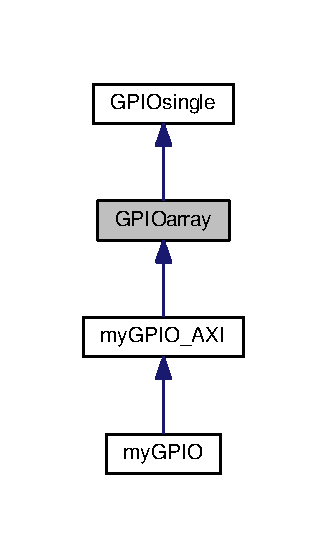
\includegraphics[width=157pt]{class_g_p_i_oarray__inherit__graph}
\end{center}
\end{figure}


Collaboration diagram for G\+P\+I\+Oarray\+:
\nopagebreak
\begin{figure}[H]
\begin{center}
\leavevmode
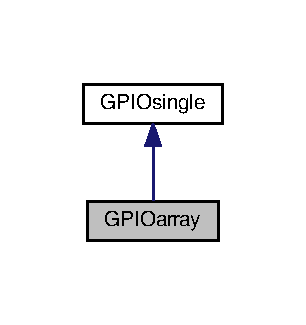
\includegraphics[width=147pt]{class_g_p_i_oarray__coll__graph}
\end{center}
\end{figure}
\subsection*{Entities}
\begin{DoxyCompactItemize}
\item 
\hyperlink{class_g_p_i_oarray_1_1_structural}{Structural} architecture
\end{DoxyCompactItemize}
\subsection*{Libraries}
 \begin{DoxyCompactItemize}
\item 
\hypertarget{class_g_p_i_oarray_ga0a6af6eef40212dbaf130d57ce711256}{\hyperlink{group__my_g_p_i_o_ga0a6af6eef40212dbaf130d57ce711256}{ieee} }\label{class_g_p_i_oarray_ga0a6af6eef40212dbaf130d57ce711256}

\end{DoxyCompactItemize}
\subsection*{Use Clauses}
 \begin{DoxyCompactItemize}
\item 
\hypertarget{class_g_p_i_oarray_gacd03516902501cd1c7296a98e22c6fcb}{\hyperlink{group__my_g_p_i_o_gacd03516902501cd1c7296a98e22c6fcb}{std\+\_\+logic\+\_\+1164}   }\label{class_g_p_i_oarray_gacd03516902501cd1c7296a98e22c6fcb}

\end{DoxyCompactItemize}
\subsection*{Generics}
 \begin{DoxyCompactItemize}
\item 
\hypertarget{class_g_p_i_oarray_ga0b52ca75e9a6093b2b60d5e851803069}{\hyperlink{group__my_g_p_i_o_ga0b52ca75e9a6093b2b60d5e851803069}{G\+P\+I\+O\+\_\+width} {\bfseries {\bfseries \textcolor{vhdlchar}{natural}\textcolor{vhdlchar}{ }\textcolor{vhdlchar}{ }\textcolor{vhdlchar}{\+:}\textcolor{vhdlchar}{=}\textcolor{vhdlchar}{ }\textcolor{vhdlchar}{ } \textcolor{vhdldigit}{4} \textcolor{vhdlchar}{ }}}}\label{class_g_p_i_oarray_ga0b52ca75e9a6093b2b60d5e851803069}

\begin{DoxyCompactList}\small\item\em parallelismo dell'array, di default pari a 4 celle. \end{DoxyCompactList}\end{DoxyCompactItemize}
\subsection*{Ports}
 \begin{DoxyCompactItemize}
\item 
\hypertarget{class_g_p_i_oarray_ga11dd30ea6a502615af8dccf7a8bc78fe}{\hyperlink{group__my_g_p_i_o_ga11dd30ea6a502615af8dccf7a8bc78fe}{G\+P\+I\+O\+\_\+enable}  {\bfseries {\bfseries \textcolor{vhdlchar}{in}\textcolor{vhdlchar}{ }}} {\bfseries \textcolor{vhdlchar}{std\+\_\+logic\+\_\+vector}\textcolor{vhdlchar}{ }\textcolor{vhdlchar}{(}\textcolor{vhdlchar}{ }\textcolor{vhdlchar}{ }\textcolor{vhdlchar}{ }\textcolor{vhdlchar}{ }{\bfseries \hyperlink{group__my_g_p_i_o_ga0b52ca75e9a6093b2b60d5e851803069}{G\+P\+I\+O\+\_\+width}} \textcolor{vhdlchar}{-\/}\textcolor{vhdlchar}{ } \textcolor{vhdldigit}{1} \textcolor{vhdlchar}{ }\textcolor{vhdlchar}{downto}\textcolor{vhdlchar}{ }\textcolor{vhdlchar}{ } \textcolor{vhdldigit}{0} \textcolor{vhdlchar}{ }\textcolor{vhdlchar}{)}\textcolor{vhdlchar}{ }} }\label{class_g_p_i_oarray_ga11dd30ea6a502615af8dccf7a8bc78fe}

\begin{DoxyCompactList}\small\item\em segnale di abilitazione, permette di pilotare la linea \char`\"{}\+G\+P\+I\+O\+\_\+inout\char`\"{}. Quando G\+P\+I\+O\+\_\+enable=1, la linea G\+P\+I\+O\+\_\+inout e quella G\+P\+I\+O\+\_\+write sono connesse tra loro. \end{DoxyCompactList}\item 
\hypertarget{class_g_p_i_oarray_ga15a2a96cc1645c826c8ac6469f70c5c0}{\hyperlink{group__my_g_p_i_o_ga15a2a96cc1645c826c8ac6469f70c5c0}{G\+P\+I\+O\+\_\+write}  {\bfseries {\bfseries \textcolor{vhdlchar}{in}\textcolor{vhdlchar}{ }}} {\bfseries \textcolor{vhdlchar}{std\+\_\+logic\+\_\+vector}\textcolor{vhdlchar}{ }\textcolor{vhdlchar}{(}\textcolor{vhdlchar}{ }\textcolor{vhdlchar}{ }\textcolor{vhdlchar}{ }\textcolor{vhdlchar}{ }{\bfseries \hyperlink{group__my_g_p_i_o_ga0b52ca75e9a6093b2b60d5e851803069}{G\+P\+I\+O\+\_\+width}} \textcolor{vhdlchar}{-\/}\textcolor{vhdlchar}{ } \textcolor{vhdldigit}{1} \textcolor{vhdlchar}{ }\textcolor{vhdlchar}{downto}\textcolor{vhdlchar}{ }\textcolor{vhdlchar}{ } \textcolor{vhdldigit}{0} \textcolor{vhdlchar}{ }\textcolor{vhdlchar}{)}\textcolor{vhdlchar}{ }} }\label{class_g_p_i_oarray_ga15a2a96cc1645c826c8ac6469f70c5c0}

\begin{DoxyCompactList}\small\item\em segnale di input, diretto verso l'esterno del device. \end{DoxyCompactList}\item 
\hypertarget{class_g_p_i_oarray_ga8829699d739ef35a4c5da396ffd38387}{\hyperlink{group__my_g_p_i_o_ga8829699d739ef35a4c5da396ffd38387}{G\+P\+I\+O\+\_\+inout}  {\bfseries {\bfseries \textcolor{vhdlchar}{inout}\textcolor{vhdlchar}{ }}} {\bfseries \textcolor{vhdlchar}{std\+\_\+logic\+\_\+vector}\textcolor{vhdlchar}{ }\textcolor{vhdlchar}{(}\textcolor{vhdlchar}{ }\textcolor{vhdlchar}{ }\textcolor{vhdlchar}{ }\textcolor{vhdlchar}{ }{\bfseries \hyperlink{group__my_g_p_i_o_ga0b52ca75e9a6093b2b60d5e851803069}{G\+P\+I\+O\+\_\+width}} \textcolor{vhdlchar}{-\/}\textcolor{vhdlchar}{ } \textcolor{vhdldigit}{1} \textcolor{vhdlchar}{ }\textcolor{vhdlchar}{downto}\textcolor{vhdlchar}{ }\textcolor{vhdlchar}{ } \textcolor{vhdldigit}{0} \textcolor{vhdlchar}{ }\textcolor{vhdlchar}{)}\textcolor{vhdlchar}{ }} }\label{class_g_p_i_oarray_ga8829699d739ef35a4c5da396ffd38387}

\begin{DoxyCompactList}\small\item\em segnale bidirezionale diretto verso l'esterno del device. \end{DoxyCompactList}\item 
\hypertarget{class_g_p_i_oarray_gafbe6792efd02cef42af7717592c1b04a}{\hyperlink{group__my_g_p_i_o_gafbe6792efd02cef42af7717592c1b04a}{G\+P\+I\+O\+\_\+read}  {\bfseries {\bfseries \textcolor{vhdlchar}{out}\textcolor{vhdlchar}{ }}} {\bfseries \textcolor{vhdlchar}{std\+\_\+logic\+\_\+vector}\textcolor{vhdlchar}{ }\textcolor{vhdlchar}{(}\textcolor{vhdlchar}{ }\textcolor{vhdlchar}{ }\textcolor{vhdlchar}{ }\textcolor{vhdlchar}{ }{\bfseries \hyperlink{group__my_g_p_i_o_ga0b52ca75e9a6093b2b60d5e851803069}{G\+P\+I\+O\+\_\+width}} \textcolor{vhdlchar}{-\/}\textcolor{vhdlchar}{ } \textcolor{vhdldigit}{1} \textcolor{vhdlchar}{ }\textcolor{vhdlchar}{downto}\textcolor{vhdlchar}{ }\textcolor{vhdlchar}{ } \textcolor{vhdldigit}{0} \textcolor{vhdlchar}{ }\textcolor{vhdlchar}{)}\textcolor{vhdlchar}{ }} }\label{class_g_p_i_oarray_gafbe6792efd02cef42af7717592c1b04a}

\begin{DoxyCompactList}\small\item\em segnale di output, diretto verso l'interno del device. \end{DoxyCompactList}\end{DoxyCompactItemize}


\subsection{Detailed Description}
array di celle G\+P\+I\+O, pilotabili singolarmente 

The documentation for this class was generated from the following file\+:\begin{DoxyCompactItemize}
\item 
\hyperlink{_g_p_i_oarray_8vhd}{G\+P\+I\+Oarray.\+vhd}\end{DoxyCompactItemize}

\hypertarget{class_g_p_i_osingle}{\section{G\+P\+I\+Osingle Entity Reference}
\label{class_g_p_i_osingle}\index{G\+P\+I\+Osingle@{G\+P\+I\+Osingle}}
}


Cella base G\+P\+I\+O.  




Diagramma delle classi per G\+P\+I\+Osingle\nopagebreak
\begin{figure}[H]
\begin{center}
\leavevmode
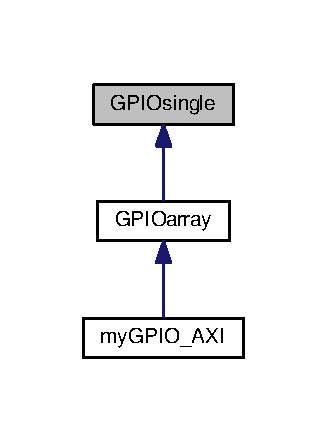
\includegraphics[width=157pt]{class_g_p_i_osingle__inherit__graph}
\end{center}
\end{figure}
\subsection*{Entities}
\begin{DoxyCompactItemize}
\item 
\hyperlink{class_g_p_i_osingle_1_1_structural}{Structural} architecture
\end{DoxyCompactItemize}
\subsection*{Libraries}
 \begin{DoxyCompactItemize}
\item 
\hypertarget{class_g_p_i_osingle_ga0a6af6eef40212dbaf130d57ce711256}{\hyperlink{group___g_p_i_o-single_ga0a6af6eef40212dbaf130d57ce711256}{ieee} }\label{class_g_p_i_osingle_ga0a6af6eef40212dbaf130d57ce711256}

\end{DoxyCompactItemize}
\subsection*{Use Clauses}
 \begin{DoxyCompactItemize}
\item 
\hypertarget{class_g_p_i_osingle_gacd03516902501cd1c7296a98e22c6fcb}{\hyperlink{group___g_p_i_o-single_gacd03516902501cd1c7296a98e22c6fcb}{std\+\_\+logic\+\_\+1164}   }\label{class_g_p_i_osingle_gacd03516902501cd1c7296a98e22c6fcb}

\end{DoxyCompactItemize}
\subsection*{Ports}
 \begin{DoxyCompactItemize}
\item 
\hypertarget{class_g_p_i_osingle_ga0ae7f62d9fa2c19d7ad2ad7574b58871}{\hyperlink{group___g_p_i_o-single_ga0ae7f62d9fa2c19d7ad2ad7574b58871}{G\+P\+I\+O\+\_\+enable}  {\bfseries {\bfseries \textcolor{vhdlchar}{in}\textcolor{vhdlchar}{ }}} {\bfseries \textcolor{vhdlchar}{std\+\_\+logic}\textcolor{vhdlchar}{ }} }\label{class_g_p_i_osingle_ga0ae7f62d9fa2c19d7ad2ad7574b58871}

\begin{DoxyCompactList}\small\item\em segnale di abilitazione, permette di pilotare la linea \char`\"{}\+G\+P\+I\+O\+\_\+inout\char`\"{}. Quando G\+P\+I\+O\+\_\+enable=1, la linea G\+P\+I\+O\+\_\+inout e quella G\+P\+I\+O\+\_\+write sono connesse tra loro, consentendo la scrittura del valore del segnale G\+P\+I\+O\+\_\+inout \end{DoxyCompactList}\item 
\hypertarget{class_g_p_i_osingle_ga20547939f304c722cb29df650d7ca7ef}{\hyperlink{group___g_p_i_o-single_ga20547939f304c722cb29df650d7ca7ef}{G\+P\+I\+O\+\_\+write}  {\bfseries {\bfseries \textcolor{vhdlchar}{in}\textcolor{vhdlchar}{ }}} {\bfseries \textcolor{vhdlchar}{std\+\_\+logic}\textcolor{vhdlchar}{ }} }\label{class_g_p_i_osingle_ga20547939f304c722cb29df650d7ca7ef}

\begin{DoxyCompactList}\small\item\em segnale di input, diretto verso l'esterno del device \hyperlink{class_g_p_i_osingle}{G\+P\+I\+Osingle}. Quando G\+P\+I\+O\+\_\+enable=1, la linea G\+P\+I\+O\+\_\+inout e quella G\+P\+I\+O\+\_\+write sono connesse tra loro, consentendo la scrittura del valore del pin G\+P\+I\+O\+\_\+inout. \end{DoxyCompactList}\item 
\hypertarget{class_g_p_i_osingle_ga979707b3e6ce3920d653c07c91e80f70}{\hyperlink{group___g_p_i_o-single_ga979707b3e6ce3920d653c07c91e80f70}{G\+P\+I\+O\+\_\+inout}  {\bfseries {\bfseries \textcolor{vhdlchar}{inout}\textcolor{vhdlchar}{ }}} {\bfseries \textcolor{vhdlchar}{std\+\_\+logic}\textcolor{vhdlchar}{ }} }\label{class_g_p_i_osingle_ga979707b3e6ce3920d653c07c91e80f70}

\begin{DoxyCompactList}\small\item\em segnale bidirezionale diretto verso l'esterno del device. Può essere usato per leggere/scrivere segnali digitali da/verso l'esterno del device \hyperlink{class_g_p_i_osingle}{G\+P\+I\+Osingle} \end{DoxyCompactList}\item 
\hypertarget{class_g_p_i_osingle_ga4a6632a5d5cd6c4e6c1b634286795362}{\hyperlink{group___g_p_i_o-single_ga4a6632a5d5cd6c4e6c1b634286795362}{G\+P\+I\+O\+\_\+read}  {\bfseries {\bfseries \textcolor{vhdlchar}{out}\textcolor{vhdlchar}{ }}} {\bfseries \textcolor{vhdlchar}{std\+\_\+logic}\textcolor{vhdlchar}{ }} }\label{class_g_p_i_osingle_ga4a6632a5d5cd6c4e6c1b634286795362}

\begin{DoxyCompactList}\small\item\em segnale di output, diretto verso l'esterno del device. Quando G\+P\+I\+O\+\_\+enable=1, la linea G\+P\+I\+O\+\_\+inout e quella G\+P\+I\+O\+\_\+write sono connesse tra loro, consentendo la scrittura del valore dei pin, per cui questo segnale assume esattamente il valore con cui viene impostato il segnale G\+P\+I\+O\+\_\+write \end{DoxyCompactList}\end{DoxyCompactItemize}


\subsection{Descrizione dettagliata}
Cella base G\+P\+I\+O. 

La documentazione per questa classe è stata generata a partire dal seguente file\+:\begin{DoxyCompactItemize}
\item 
Src/my\+G\+P\+I\+O/\+V\+H\+D\+L/\hyperlink{_g_p_i_osingle_8vhd}{G\+P\+I\+Osingle.\+vhd}\end{DoxyCompactItemize}

\hypertarget{classmy_g_p_i_o}{\section{my\+G\+P\+I\+O Entity Reference}
\label{classmy_g_p_i_o}\index{my\+G\+P\+I\+O@{my\+G\+P\+I\+O}}
}
\subsection*{Libraries}
 \begin{DoxyCompactItemize}
\item 
\hypertarget{classmy_g_p_i_o_ga0a6af6eef40212dbaf130d57ce711256}{\hyperlink{group___a_x_i-device_ga0a6af6eef40212dbaf130d57ce711256}{ieee} }\label{classmy_g_p_i_o_ga0a6af6eef40212dbaf130d57ce711256}

\end{DoxyCompactItemize}
\subsection*{Use Clauses}
 \begin{DoxyCompactItemize}
\item 
\hypertarget{classmy_g_p_i_o_gacd03516902501cd1c7296a98e22c6fcb}{\hyperlink{group___a_x_i-device_gacd03516902501cd1c7296a98e22c6fcb}{std\+\_\+logic\+\_\+1164}   }\label{classmy_g_p_i_o_gacd03516902501cd1c7296a98e22c6fcb}

\item 
\hypertarget{classmy_g_p_i_o_ga2edc34402b573437d5f25fa90ba4013e}{\hyperlink{group___a_x_i-device_ga2edc34402b573437d5f25fa90ba4013e}{numeric\+\_\+std}   }\label{classmy_g_p_i_o_ga2edc34402b573437d5f25fa90ba4013e}

\end{DoxyCompactItemize}
\subsection*{Generics}
 \begin{DoxyCompactItemize}
\item 
\hypertarget{classmy_g_p_i_o_ga0b52ca75e9a6093b2b60d5e851803069}{\hyperlink{group___a_x_i-device_ga0b52ca75e9a6093b2b60d5e851803069}{G\+P\+I\+O\+\_\+width} {\bfseries {\bfseries \textcolor{vhdlchar}{natural}\textcolor{vhdlchar}{ }\textcolor{vhdlchar}{ }\textcolor{vhdlchar}{\+:}\textcolor{vhdlchar}{=}\textcolor{vhdlchar}{ }\textcolor{vhdlchar}{ } \textcolor{vhdldigit}{4} \textcolor{vhdlchar}{ }}}}\label{classmy_g_p_i_o_ga0b52ca75e9a6093b2b60d5e851803069}

\begin{DoxyCompactList}\small\item\em numero di G\+P\+I\+O offerti dalla periferica, di default pari a 4 celle. \end{DoxyCompactList}\item 
\hypertarget{classmy_g_p_i_o_gafce7943994a4ddfa81f224225976a4c7}{\hyperlink{group___a_x_i-device_gafce7943994a4ddfa81f224225976a4c7}{C\+\_\+\+S00\+\_\+\+A\+X\+I\+\_\+\+D\+A\+T\+A\+\_\+\+W\+I\+D\+T\+H} {\bfseries {\bfseries \textcolor{vhdlchar}{integer}\textcolor{vhdlchar}{ }\textcolor{vhdlchar}{ }\textcolor{vhdlchar}{\+:}\textcolor{vhdlchar}{=}\textcolor{vhdlchar}{ }\textcolor{vhdlchar}{ } \textcolor{vhdldigit}{32} \textcolor{vhdlchar}{ }}}}\label{classmy_g_p_i_o_gafce7943994a4ddfa81f224225976a4c7}

\begin{DoxyCompactList}\small\item\em \end{DoxyCompactList}\item 
\hypertarget{classmy_g_p_i_o_gab7787f274c76bb896ac98fdcfb570c65}{\hyperlink{group___a_x_i-device_gab7787f274c76bb896ac98fdcfb570c65}{C\+\_\+\+S00\+\_\+\+A\+X\+I\+\_\+\+A\+D\+D\+R\+\_\+\+W\+I\+D\+T\+H} {\bfseries {\bfseries \textcolor{vhdlchar}{integer}\textcolor{vhdlchar}{ }\textcolor{vhdlchar}{ }\textcolor{vhdlchar}{\+:}\textcolor{vhdlchar}{=}\textcolor{vhdlchar}{ }\textcolor{vhdlchar}{ } \textcolor{vhdldigit}{5} \textcolor{vhdlchar}{ }}}}\label{classmy_g_p_i_o_gab7787f274c76bb896ac98fdcfb570c65}

\begin{DoxyCompactList}\small\item\em \end{DoxyCompactList}\end{DoxyCompactItemize}
\subsection*{Ports}
 \begin{DoxyCompactItemize}
\item 
\hypertarget{classmy_g_p_i_o_ga8829699d739ef35a4c5da396ffd38387}{\hyperlink{group___a_x_i-device_ga8829699d739ef35a4c5da396ffd38387}{G\+P\+I\+O\+\_\+inout}  {\bfseries {\bfseries \textcolor{vhdlchar}{inout}\textcolor{vhdlchar}{ }}} {\bfseries \textcolor{vhdlchar}{std\+\_\+logic\+\_\+vector}\textcolor{vhdlchar}{ }\textcolor{vhdlchar}{(}\textcolor{vhdlchar}{ }\textcolor{vhdlchar}{ }\textcolor{vhdlchar}{ }\textcolor{vhdlchar}{ }{\bfseries \hyperlink{group___a_x_i-device_ga0b52ca75e9a6093b2b60d5e851803069}{G\+P\+I\+O\+\_\+width}} \textcolor{vhdlchar}{-\/}\textcolor{vhdlchar}{ } \textcolor{vhdldigit}{1} \textcolor{vhdlchar}{ }\textcolor{vhdlchar}{downto}\textcolor{vhdlchar}{ }\textcolor{vhdlchar}{ } \textcolor{vhdldigit}{0} \textcolor{vhdlchar}{ }\textcolor{vhdlchar}{)}\textcolor{vhdlchar}{ }} }\label{classmy_g_p_i_o_ga8829699d739ef35a4c5da396ffd38387}

\begin{DoxyCompactList}\small\item\em segnale bidirezionale diretto verso l'esterno del device. \end{DoxyCompactList}\item 
\hypertarget{classmy_g_p_i_o_ga5b78f3e3edfaf6e8ec79031b9e631e9d}{\hyperlink{group___a_x_i-device_ga5b78f3e3edfaf6e8ec79031b9e631e9d}{interrupt}  {\bfseries {\bfseries \textcolor{vhdlchar}{out}\textcolor{vhdlchar}{ }}} {\bfseries \textcolor{vhdlchar}{std\+\_\+logic}\textcolor{vhdlchar}{ }} }\label{classmy_g_p_i_o_ga5b78f3e3edfaf6e8ec79031b9e631e9d}

\begin{DoxyCompactList}\small\item\em segnale di interrupt a livelli diretto verso il processing -\/ system. Se le interruzioni sono abilitate ed uno dei pin del device è settato come input ed è abilitato a generare interruzioni, diventa '1' appena tale pin assume valore '1', e mantiene tale valore fino a quando tutte le interruzioni non siano state servite. \end{DoxyCompactList}\item 
\hypertarget{classmy_g_p_i_o_ga037f9e3df8559bfd59db37bcba9cb7a8}{\hyperlink{group___a_x_i-device_ga037f9e3df8559bfd59db37bcba9cb7a8}{s00\+\_\+axi\+\_\+aclk}  {\bfseries {\bfseries \textcolor{vhdlchar}{in}\textcolor{vhdlchar}{ }}} {\bfseries \textcolor{vhdlchar}{std\+\_\+logic}\textcolor{vhdlchar}{ }} }\label{classmy_g_p_i_o_ga037f9e3df8559bfd59db37bcba9cb7a8}

\begin{DoxyCompactList}\small\item\em \end{DoxyCompactList}\item 
\hypertarget{classmy_g_p_i_o_ga8249c106fbd80196dcad2666c9f0b3fc}{\hyperlink{group___a_x_i-device_ga8249c106fbd80196dcad2666c9f0b3fc}{s00\+\_\+axi\+\_\+aresetn}  {\bfseries {\bfseries \textcolor{vhdlchar}{in}\textcolor{vhdlchar}{ }}} {\bfseries \textcolor{vhdlchar}{std\+\_\+logic}\textcolor{vhdlchar}{ }} }\label{classmy_g_p_i_o_ga8249c106fbd80196dcad2666c9f0b3fc}

\item 
\hypertarget{classmy_g_p_i_o_ga9fe80d3cc7f862afb670536e4e05dbeb}{\hyperlink{group___a_x_i-device_ga9fe80d3cc7f862afb670536e4e05dbeb}{s00\+\_\+axi\+\_\+awaddr}  {\bfseries {\bfseries \textcolor{vhdlchar}{in}\textcolor{vhdlchar}{ }}} {\bfseries \textcolor{vhdlchar}{std\+\_\+logic\+\_\+vector}\textcolor{vhdlchar}{ }\textcolor{vhdlchar}{(}\textcolor{vhdlchar}{ }\textcolor{vhdlchar}{ }\textcolor{vhdlchar}{ }\textcolor{vhdlchar}{ }{\bfseries \hyperlink{group___a_x_i-device_gab7787f274c76bb896ac98fdcfb570c65}{C\+\_\+\+S00\+\_\+\+A\+X\+I\+\_\+\+A\+D\+D\+R\+\_\+\+W\+I\+D\+T\+H}} \textcolor{vhdlchar}{-\/}\textcolor{vhdlchar}{ } \textcolor{vhdldigit}{1} \textcolor{vhdlchar}{ }\textcolor{vhdlchar}{downto}\textcolor{vhdlchar}{ }\textcolor{vhdlchar}{ } \textcolor{vhdldigit}{0} \textcolor{vhdlchar}{ }\textcolor{vhdlchar}{)}\textcolor{vhdlchar}{ }} }\label{classmy_g_p_i_o_ga9fe80d3cc7f862afb670536e4e05dbeb}

\item 
\hypertarget{classmy_g_p_i_o_ga719659c1addef5432978cc949d9e10ed}{\hyperlink{group___a_x_i-device_ga719659c1addef5432978cc949d9e10ed}{s00\+\_\+axi\+\_\+awprot}  {\bfseries {\bfseries \textcolor{vhdlchar}{in}\textcolor{vhdlchar}{ }}} {\bfseries \textcolor{vhdlchar}{std\+\_\+logic\+\_\+vector}\textcolor{vhdlchar}{ }\textcolor{vhdlchar}{(}\textcolor{vhdlchar}{ }\textcolor{vhdlchar}{ } \textcolor{vhdldigit}{2} \textcolor{vhdlchar}{ }\textcolor{vhdlchar}{downto}\textcolor{vhdlchar}{ }\textcolor{vhdlchar}{ } \textcolor{vhdldigit}{0} \textcolor{vhdlchar}{ }\textcolor{vhdlchar}{)}\textcolor{vhdlchar}{ }} }\label{classmy_g_p_i_o_ga719659c1addef5432978cc949d9e10ed}

\item 
\hypertarget{classmy_g_p_i_o_ga45aa02a72ae1a8389346d47173c60ed0}{\hyperlink{group___a_x_i-device_ga45aa02a72ae1a8389346d47173c60ed0}{s00\+\_\+axi\+\_\+awvalid}  {\bfseries {\bfseries \textcolor{vhdlchar}{in}\textcolor{vhdlchar}{ }}} {\bfseries \textcolor{vhdlchar}{std\+\_\+logic}\textcolor{vhdlchar}{ }} }\label{classmy_g_p_i_o_ga45aa02a72ae1a8389346d47173c60ed0}

\item 
\hypertarget{classmy_g_p_i_o_gad0a1f71502d91a45dbc6c365f85c6566}{\hyperlink{group___a_x_i-device_gad0a1f71502d91a45dbc6c365f85c6566}{s00\+\_\+axi\+\_\+awready}  {\bfseries {\bfseries \textcolor{vhdlchar}{out}\textcolor{vhdlchar}{ }}} {\bfseries \textcolor{vhdlchar}{std\+\_\+logic}\textcolor{vhdlchar}{ }} }\label{classmy_g_p_i_o_gad0a1f71502d91a45dbc6c365f85c6566}

\item 
\hypertarget{classmy_g_p_i_o_gae2b15b55ee463fd9dd030ee29db6bb17}{\hyperlink{group___a_x_i-device_gae2b15b55ee463fd9dd030ee29db6bb17}{s00\+\_\+axi\+\_\+wdata}  {\bfseries {\bfseries \textcolor{vhdlchar}{in}\textcolor{vhdlchar}{ }}} {\bfseries \textcolor{vhdlchar}{std\+\_\+logic\+\_\+vector}\textcolor{vhdlchar}{ }\textcolor{vhdlchar}{(}\textcolor{vhdlchar}{ }\textcolor{vhdlchar}{ }\textcolor{vhdlchar}{ }\textcolor{vhdlchar}{ }{\bfseries \hyperlink{group___a_x_i-device_gafce7943994a4ddfa81f224225976a4c7}{C\+\_\+\+S00\+\_\+\+A\+X\+I\+\_\+\+D\+A\+T\+A\+\_\+\+W\+I\+D\+T\+H}} \textcolor{vhdlchar}{-\/}\textcolor{vhdlchar}{ } \textcolor{vhdldigit}{1} \textcolor{vhdlchar}{ }\textcolor{vhdlchar}{downto}\textcolor{vhdlchar}{ }\textcolor{vhdlchar}{ } \textcolor{vhdldigit}{0} \textcolor{vhdlchar}{ }\textcolor{vhdlchar}{)}\textcolor{vhdlchar}{ }} }\label{classmy_g_p_i_o_gae2b15b55ee463fd9dd030ee29db6bb17}

\item 
\hypertarget{classmy_g_p_i_o_ga120924bc3fd5fd10ec0f96e19c3f4904}{\hyperlink{group___a_x_i-device_ga120924bc3fd5fd10ec0f96e19c3f4904}{s00\+\_\+axi\+\_\+wstrb}  {\bfseries {\bfseries \textcolor{vhdlchar}{in}\textcolor{vhdlchar}{ }}} {\bfseries \textcolor{vhdlchar}{std\+\_\+logic\+\_\+vector}\textcolor{vhdlchar}{ }\textcolor{vhdlchar}{(}\textcolor{vhdlchar}{ }\textcolor{vhdlchar}{(}\textcolor{vhdlchar}{ }\textcolor{vhdlchar}{ }\textcolor{vhdlchar}{ }\textcolor{vhdlchar}{ }{\bfseries \hyperlink{group___a_x_i-device_gafce7943994a4ddfa81f224225976a4c7}{C\+\_\+\+S00\+\_\+\+A\+X\+I\+\_\+\+D\+A\+T\+A\+\_\+\+W\+I\+D\+T\+H}} \textcolor{vhdlchar}{/}\textcolor{vhdlchar}{ } \textcolor{vhdldigit}{8} \textcolor{vhdlchar}{ }\textcolor{vhdlchar}{)}\textcolor{vhdlchar}{ }\textcolor{vhdlchar}{-\/}\textcolor{vhdlchar}{ } \textcolor{vhdldigit}{1} \textcolor{vhdlchar}{ }\textcolor{vhdlchar}{downto}\textcolor{vhdlchar}{ }\textcolor{vhdlchar}{ } \textcolor{vhdldigit}{0} \textcolor{vhdlchar}{ }\textcolor{vhdlchar}{)}\textcolor{vhdlchar}{ }} }\label{classmy_g_p_i_o_ga120924bc3fd5fd10ec0f96e19c3f4904}

\item 
\hypertarget{classmy_g_p_i_o_ga24e90907193647007d2947353740114d}{\hyperlink{group___a_x_i-device_ga24e90907193647007d2947353740114d}{s00\+\_\+axi\+\_\+wvalid}  {\bfseries {\bfseries \textcolor{vhdlchar}{in}\textcolor{vhdlchar}{ }}} {\bfseries \textcolor{vhdlchar}{std\+\_\+logic}\textcolor{vhdlchar}{ }} }\label{classmy_g_p_i_o_ga24e90907193647007d2947353740114d}

\item 
\hypertarget{classmy_g_p_i_o_ga3fc60abc0cfbfa90003a83bffdd476c4}{\hyperlink{group___a_x_i-device_ga3fc60abc0cfbfa90003a83bffdd476c4}{s00\+\_\+axi\+\_\+wready}  {\bfseries {\bfseries \textcolor{vhdlchar}{out}\textcolor{vhdlchar}{ }}} {\bfseries \textcolor{vhdlchar}{std\+\_\+logic}\textcolor{vhdlchar}{ }} }\label{classmy_g_p_i_o_ga3fc60abc0cfbfa90003a83bffdd476c4}

\item 
\hypertarget{classmy_g_p_i_o_gaf8799be946d3f5354263e7deb15f94f1}{\hyperlink{group___a_x_i-device_gaf8799be946d3f5354263e7deb15f94f1}{s00\+\_\+axi\+\_\+bresp}  {\bfseries {\bfseries \textcolor{vhdlchar}{out}\textcolor{vhdlchar}{ }}} {\bfseries \textcolor{vhdlchar}{std\+\_\+logic\+\_\+vector}\textcolor{vhdlchar}{ }\textcolor{vhdlchar}{(}\textcolor{vhdlchar}{ }\textcolor{vhdlchar}{ } \textcolor{vhdldigit}{1} \textcolor{vhdlchar}{ }\textcolor{vhdlchar}{downto}\textcolor{vhdlchar}{ }\textcolor{vhdlchar}{ } \textcolor{vhdldigit}{0} \textcolor{vhdlchar}{ }\textcolor{vhdlchar}{)}\textcolor{vhdlchar}{ }} }\label{classmy_g_p_i_o_gaf8799be946d3f5354263e7deb15f94f1}

\item 
\hypertarget{classmy_g_p_i_o_ga5110b7dd4fb9548a2aab88f50dbe1d5e}{\hyperlink{group___a_x_i-device_ga5110b7dd4fb9548a2aab88f50dbe1d5e}{s00\+\_\+axi\+\_\+bvalid}  {\bfseries {\bfseries \textcolor{vhdlchar}{out}\textcolor{vhdlchar}{ }}} {\bfseries \textcolor{vhdlchar}{std\+\_\+logic}\textcolor{vhdlchar}{ }} }\label{classmy_g_p_i_o_ga5110b7dd4fb9548a2aab88f50dbe1d5e}

\item 
\hypertarget{classmy_g_p_i_o_ga1ef2019b0613bc23d4829eeeb24eb98d}{\hyperlink{group___a_x_i-device_ga1ef2019b0613bc23d4829eeeb24eb98d}{s00\+\_\+axi\+\_\+bready}  {\bfseries {\bfseries \textcolor{vhdlchar}{in}\textcolor{vhdlchar}{ }}} {\bfseries \textcolor{vhdlchar}{std\+\_\+logic}\textcolor{vhdlchar}{ }} }\label{classmy_g_p_i_o_ga1ef2019b0613bc23d4829eeeb24eb98d}

\item 
\hypertarget{classmy_g_p_i_o_gaf70a86336cd6505064e45b69f4623939}{\hyperlink{group___a_x_i-device_gaf70a86336cd6505064e45b69f4623939}{s00\+\_\+axi\+\_\+araddr}  {\bfseries {\bfseries \textcolor{vhdlchar}{in}\textcolor{vhdlchar}{ }}} {\bfseries \textcolor{vhdlchar}{std\+\_\+logic\+\_\+vector}\textcolor{vhdlchar}{ }\textcolor{vhdlchar}{(}\textcolor{vhdlchar}{ }\textcolor{vhdlchar}{ }\textcolor{vhdlchar}{ }\textcolor{vhdlchar}{ }{\bfseries \hyperlink{group___a_x_i-device_gab7787f274c76bb896ac98fdcfb570c65}{C\+\_\+\+S00\+\_\+\+A\+X\+I\+\_\+\+A\+D\+D\+R\+\_\+\+W\+I\+D\+T\+H}} \textcolor{vhdlchar}{-\/}\textcolor{vhdlchar}{ } \textcolor{vhdldigit}{1} \textcolor{vhdlchar}{ }\textcolor{vhdlchar}{downto}\textcolor{vhdlchar}{ }\textcolor{vhdlchar}{ } \textcolor{vhdldigit}{0} \textcolor{vhdlchar}{ }\textcolor{vhdlchar}{)}\textcolor{vhdlchar}{ }} }\label{classmy_g_p_i_o_gaf70a86336cd6505064e45b69f4623939}

\item 
\hypertarget{classmy_g_p_i_o_gadc648df07895bf808b8c721e1dc6811b}{\hyperlink{group___a_x_i-device_gadc648df07895bf808b8c721e1dc6811b}{s00\+\_\+axi\+\_\+arprot}  {\bfseries {\bfseries \textcolor{vhdlchar}{in}\textcolor{vhdlchar}{ }}} {\bfseries \textcolor{vhdlchar}{std\+\_\+logic\+\_\+vector}\textcolor{vhdlchar}{ }\textcolor{vhdlchar}{(}\textcolor{vhdlchar}{ }\textcolor{vhdlchar}{ } \textcolor{vhdldigit}{2} \textcolor{vhdlchar}{ }\textcolor{vhdlchar}{downto}\textcolor{vhdlchar}{ }\textcolor{vhdlchar}{ } \textcolor{vhdldigit}{0} \textcolor{vhdlchar}{ }\textcolor{vhdlchar}{)}\textcolor{vhdlchar}{ }} }\label{classmy_g_p_i_o_gadc648df07895bf808b8c721e1dc6811b}

\item 
\hypertarget{classmy_g_p_i_o_ga94b78b2ae3cd13860f15afbdfb199e44}{\hyperlink{group___a_x_i-device_ga94b78b2ae3cd13860f15afbdfb199e44}{s00\+\_\+axi\+\_\+arvalid}  {\bfseries {\bfseries \textcolor{vhdlchar}{in}\textcolor{vhdlchar}{ }}} {\bfseries \textcolor{vhdlchar}{std\+\_\+logic}\textcolor{vhdlchar}{ }} }\label{classmy_g_p_i_o_ga94b78b2ae3cd13860f15afbdfb199e44}

\item 
\hypertarget{classmy_g_p_i_o_gad35bd95f3352ff8dbdaea55205a98e53}{\hyperlink{group___a_x_i-device_gad35bd95f3352ff8dbdaea55205a98e53}{s00\+\_\+axi\+\_\+arready}  {\bfseries {\bfseries \textcolor{vhdlchar}{out}\textcolor{vhdlchar}{ }}} {\bfseries \textcolor{vhdlchar}{std\+\_\+logic}\textcolor{vhdlchar}{ }} }\label{classmy_g_p_i_o_gad35bd95f3352ff8dbdaea55205a98e53}

\item 
\hypertarget{classmy_g_p_i_o_gad2655fadb987e0487c428aca187b55d0}{\hyperlink{group___a_x_i-device_gad2655fadb987e0487c428aca187b55d0}{s00\+\_\+axi\+\_\+rdata}  {\bfseries {\bfseries \textcolor{vhdlchar}{out}\textcolor{vhdlchar}{ }}} {\bfseries \textcolor{vhdlchar}{std\+\_\+logic\+\_\+vector}\textcolor{vhdlchar}{ }\textcolor{vhdlchar}{(}\textcolor{vhdlchar}{ }\textcolor{vhdlchar}{ }\textcolor{vhdlchar}{ }\textcolor{vhdlchar}{ }{\bfseries \hyperlink{group___a_x_i-device_gafce7943994a4ddfa81f224225976a4c7}{C\+\_\+\+S00\+\_\+\+A\+X\+I\+\_\+\+D\+A\+T\+A\+\_\+\+W\+I\+D\+T\+H}} \textcolor{vhdlchar}{-\/}\textcolor{vhdlchar}{ } \textcolor{vhdldigit}{1} \textcolor{vhdlchar}{ }\textcolor{vhdlchar}{downto}\textcolor{vhdlchar}{ }\textcolor{vhdlchar}{ } \textcolor{vhdldigit}{0} \textcolor{vhdlchar}{ }\textcolor{vhdlchar}{)}\textcolor{vhdlchar}{ }} }\label{classmy_g_p_i_o_gad2655fadb987e0487c428aca187b55d0}

\item 
\hypertarget{classmy_g_p_i_o_ga1acee955f50f71e5595a03c6ca301cf0}{\hyperlink{group___a_x_i-device_ga1acee955f50f71e5595a03c6ca301cf0}{s00\+\_\+axi\+\_\+rresp}  {\bfseries {\bfseries \textcolor{vhdlchar}{out}\textcolor{vhdlchar}{ }}} {\bfseries \textcolor{vhdlchar}{std\+\_\+logic\+\_\+vector}\textcolor{vhdlchar}{ }\textcolor{vhdlchar}{(}\textcolor{vhdlchar}{ }\textcolor{vhdlchar}{ } \textcolor{vhdldigit}{1} \textcolor{vhdlchar}{ }\textcolor{vhdlchar}{downto}\textcolor{vhdlchar}{ }\textcolor{vhdlchar}{ } \textcolor{vhdldigit}{0} \textcolor{vhdlchar}{ }\textcolor{vhdlchar}{)}\textcolor{vhdlchar}{ }} }\label{classmy_g_p_i_o_ga1acee955f50f71e5595a03c6ca301cf0}

\item 
\hypertarget{classmy_g_p_i_o_gaf180911f7eb262e530e26865bc97aa0b}{\hyperlink{group___a_x_i-device_gaf180911f7eb262e530e26865bc97aa0b}{s00\+\_\+axi\+\_\+rvalid}  {\bfseries {\bfseries \textcolor{vhdlchar}{out}\textcolor{vhdlchar}{ }}} {\bfseries \textcolor{vhdlchar}{std\+\_\+logic}\textcolor{vhdlchar}{ }} }\label{classmy_g_p_i_o_gaf180911f7eb262e530e26865bc97aa0b}

\item 
\hypertarget{classmy_g_p_i_o_ga8b82eb165d7024f6c7b25646f6ebdd4d}{\hyperlink{group___a_x_i-device_ga8b82eb165d7024f6c7b25646f6ebdd4d}{s00\+\_\+axi\+\_\+rready}  {\bfseries {\bfseries \textcolor{vhdlchar}{in}\textcolor{vhdlchar}{ }}} {\bfseries \textcolor{vhdlchar}{std\+\_\+logic}\textcolor{vhdlchar}{ }} }\label{classmy_g_p_i_o_ga8b82eb165d7024f6c7b25646f6ebdd4d}

\begin{DoxyCompactList}\small\item\em \end{DoxyCompactList}\end{DoxyCompactItemize}


La documentazione per questa classe è stata generata a partire dal seguente file\+:\begin{DoxyCompactItemize}
\item 
Src/my\+G\+P\+I\+O/\+V\+H\+D\+L/my\+G\+P\+I\+O.\+vhd\end{DoxyCompactItemize}

\hypertarget{classmy_g_p_i_o___a_x_i}{\section{my\+G\+P\+I\+O\+\_\+\+A\+X\+I Entity Reference}
\label{classmy_g_p_i_o___a_x_i}\index{my\+G\+P\+I\+O\+\_\+\+A\+X\+I@{my\+G\+P\+I\+O\+\_\+\+A\+X\+I}}
}


Inheritance diagram for my\+G\+P\+I\+O\+\_\+\+A\+X\+I\+:
\nopagebreak
\begin{figure}[H]
\begin{center}
\leavevmode
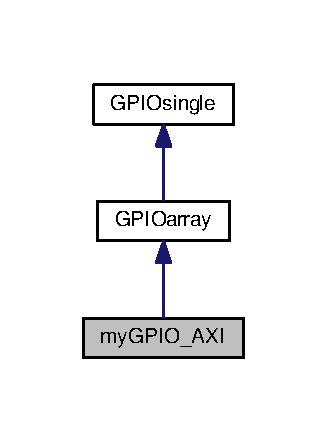
\includegraphics[width=157pt]{classmy_g_p_i_o___a_x_i__inherit__graph}
\end{center}
\end{figure}


Collaboration diagram for my\+G\+P\+I\+O\+\_\+\+A\+X\+I\+:
\nopagebreak
\begin{figure}[H]
\begin{center}
\leavevmode
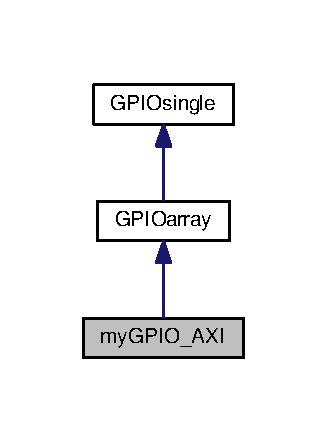
\includegraphics[width=157pt]{classmy_g_p_i_o___a_x_i__coll__graph}
\end{center}
\end{figure}
\subsection*{Entities}
\begin{DoxyCompactItemize}
\item 
\hyperlink{classmy_g_p_i_o___a_x_i_1_1arch__imp}{arch\+\_\+imp} architecture
\end{DoxyCompactItemize}
\subsection*{Libraries}
 \begin{DoxyCompactItemize}
\item 
\hypertarget{classmy_g_p_i_o___a_x_i_a0a6af6eef40212dbaf130d57ce711256}{\hyperlink{classmy_g_p_i_o___a_x_i_a0a6af6eef40212dbaf130d57ce711256}{ieee} }\label{classmy_g_p_i_o___a_x_i_a0a6af6eef40212dbaf130d57ce711256}

\end{DoxyCompactItemize}
\subsection*{Use Clauses}
 \begin{DoxyCompactItemize}
\item 
\hypertarget{classmy_g_p_i_o___a_x_i_acd03516902501cd1c7296a98e22c6fcb}{\hyperlink{classmy_g_p_i_o___a_x_i_acd03516902501cd1c7296a98e22c6fcb}{std\+\_\+logic\+\_\+1164}   }\label{classmy_g_p_i_o___a_x_i_acd03516902501cd1c7296a98e22c6fcb}

\item 
\hypertarget{classmy_g_p_i_o___a_x_i_a2edc34402b573437d5f25fa90ba4013e}{\hyperlink{classmy_g_p_i_o___a_x_i_a2edc34402b573437d5f25fa90ba4013e}{numeric\+\_\+std}   }\label{classmy_g_p_i_o___a_x_i_a2edc34402b573437d5f25fa90ba4013e}

\item 
\hypertarget{classmy_g_p_i_o___a_x_i_acb2d98d781f19c8f5f4109576ec45502}{\hyperlink{classmy_g_p_i_o___a_x_i_acb2d98d781f19c8f5f4109576ec45502}{std\+\_\+logic\+\_\+misc}   }\label{classmy_g_p_i_o___a_x_i_acb2d98d781f19c8f5f4109576ec45502}

\end{DoxyCompactItemize}
\subsection*{Generics}
 \begin{DoxyCompactItemize}
\item 
\hypertarget{classmy_g_p_i_o___a_x_i_ga0b52ca75e9a6093b2b60d5e851803069}{\hyperlink{group__my_g_p_i_o_ga0b52ca75e9a6093b2b60d5e851803069}{G\+P\+I\+O\+\_\+width} {\bfseries {\bfseries \textcolor{vhdlchar}{natural}\textcolor{vhdlchar}{ }\textcolor{vhdlchar}{ }\textcolor{vhdlchar}{\+:}\textcolor{vhdlchar}{=}\textcolor{vhdlchar}{ }\textcolor{vhdlchar}{ } \textcolor{vhdldigit}{4} \textcolor{vhdlchar}{ }}}}\label{classmy_g_p_i_o___a_x_i_ga0b52ca75e9a6093b2b60d5e851803069}

\item 
\hypertarget{classmy_g_p_i_o___a_x_i_ga0fad312acd1f302ce7de30c5658df0bd}{\hyperlink{group__my_g_p_i_o_ga0fad312acd1f302ce7de30c5658df0bd}{C\+\_\+\+S\+\_\+\+A\+X\+I\+\_\+\+D\+A\+T\+A\+\_\+\+W\+I\+D\+T\+H} {\bfseries {\bfseries \textcolor{vhdlchar}{integer}\textcolor{vhdlchar}{ }\textcolor{vhdlchar}{ }\textcolor{vhdlchar}{\+:}\textcolor{vhdlchar}{=}\textcolor{vhdlchar}{ }\textcolor{vhdlchar}{ } \textcolor{vhdldigit}{32} \textcolor{vhdlchar}{ }}}}\label{classmy_g_p_i_o___a_x_i_ga0fad312acd1f302ce7de30c5658df0bd}

\item 
\hypertarget{classmy_g_p_i_o___a_x_i_gae3f9f3251c8ea5b109c09fb14f49384c}{\hyperlink{group__my_g_p_i_o_gae3f9f3251c8ea5b109c09fb14f49384c}{C\+\_\+\+S\+\_\+\+A\+X\+I\+\_\+\+A\+D\+D\+R\+\_\+\+W\+I\+D\+T\+H} {\bfseries {\bfseries \textcolor{vhdlchar}{integer}\textcolor{vhdlchar}{ }\textcolor{vhdlchar}{ }\textcolor{vhdlchar}{\+:}\textcolor{vhdlchar}{=}\textcolor{vhdlchar}{ }\textcolor{vhdlchar}{ } \textcolor{vhdldigit}{4} \textcolor{vhdlchar}{ }}}}\label{classmy_g_p_i_o___a_x_i_gae3f9f3251c8ea5b109c09fb14f49384c}

\end{DoxyCompactItemize}
\subsection*{Ports}
 \begin{DoxyCompactItemize}
\item 
\hypertarget{classmy_g_p_i_o___a_x_i_ga8829699d739ef35a4c5da396ffd38387}{\hyperlink{group__my_g_p_i_o_ga8829699d739ef35a4c5da396ffd38387}{G\+P\+I\+O\+\_\+inout}  {\bfseries {\bfseries \textcolor{vhdlchar}{inout}\textcolor{vhdlchar}{ }}} {\bfseries \textcolor{vhdlchar}{std\+\_\+logic\+\_\+vector}\textcolor{vhdlchar}{ }\textcolor{vhdlchar}{(}\textcolor{vhdlchar}{ }\textcolor{vhdlchar}{ }\textcolor{vhdlchar}{ }\textcolor{vhdlchar}{ }\textcolor{vhdlchar}{G\+P\+I\+O\+\_\+width}\textcolor{vhdlchar}{-\/}\textcolor{vhdlchar}{ } \textcolor{vhdldigit}{1} \textcolor{vhdlchar}{ }\textcolor{vhdlchar}{downto}\textcolor{vhdlchar}{ }\textcolor{vhdlchar}{ } \textcolor{vhdldigit}{0} \textcolor{vhdlchar}{ }\textcolor{vhdlchar}{)}\textcolor{vhdlchar}{ }} }\label{classmy_g_p_i_o___a_x_i_ga8829699d739ef35a4c5da396ffd38387}

\item 
\hypertarget{classmy_g_p_i_o___a_x_i_gaa6c2451f4f1ffd390697f0b66453c2c8}{\hyperlink{group__my_g_p_i_o_gaa6c2451f4f1ffd390697f0b66453c2c8}{G\+P\+I\+O\+\_\+int}  {\bfseries {\bfseries \textcolor{vhdlchar}{out}\textcolor{vhdlchar}{ }}} {\bfseries \textcolor{vhdlchar}{std\+\_\+logic}\textcolor{vhdlchar}{ }} }\label{classmy_g_p_i_o___a_x_i_gaa6c2451f4f1ffd390697f0b66453c2c8}

\item 
\hypertarget{classmy_g_p_i_o___a_x_i_ga3f54d782a88290bdaa6baffd7cd84ab4}{\hyperlink{group__my_g_p_i_o_ga3f54d782a88290bdaa6baffd7cd84ab4}{S\+\_\+\+A\+X\+I\+\_\+\+A\+C\+L\+K}  {\bfseries {\bfseries \textcolor{vhdlchar}{in}\textcolor{vhdlchar}{ }}} {\bfseries \textcolor{vhdlchar}{std\+\_\+logic}\textcolor{vhdlchar}{ }} }\label{classmy_g_p_i_o___a_x_i_ga3f54d782a88290bdaa6baffd7cd84ab4}

\item 
\hypertarget{classmy_g_p_i_o___a_x_i_ga089b396e17dee353ccc7d5389dda5532}{\hyperlink{group__my_g_p_i_o_ga089b396e17dee353ccc7d5389dda5532}{S\+\_\+\+A\+X\+I\+\_\+\+A\+R\+E\+S\+E\+T\+N}  {\bfseries {\bfseries \textcolor{vhdlchar}{in}\textcolor{vhdlchar}{ }}} {\bfseries \textcolor{vhdlchar}{std\+\_\+logic}\textcolor{vhdlchar}{ }} }\label{classmy_g_p_i_o___a_x_i_ga089b396e17dee353ccc7d5389dda5532}

\item 
\hypertarget{classmy_g_p_i_o___a_x_i_ga61cc7b190ba9d540e56941330e4a0883}{\hyperlink{group__my_g_p_i_o_ga61cc7b190ba9d540e56941330e4a0883}{S\+\_\+\+A\+X\+I\+\_\+\+A\+W\+A\+D\+D\+R}  {\bfseries {\bfseries \textcolor{vhdlchar}{in}\textcolor{vhdlchar}{ }}} {\bfseries \textcolor{vhdlchar}{std\+\_\+logic\+\_\+vector}\textcolor{vhdlchar}{ }\textcolor{vhdlchar}{(}\textcolor{vhdlchar}{ }\textcolor{vhdlchar}{ }\textcolor{vhdlchar}{ }\textcolor{vhdlchar}{ }\textcolor{vhdlchar}{C\+\_\+\+S\+\_\+\+A\+X\+I\+\_\+\+A\+D\+D\+R\+\_\+\+W\+I\+D\+T\+H}\textcolor{vhdlchar}{-\/}\textcolor{vhdlchar}{ } \textcolor{vhdldigit}{1} \textcolor{vhdlchar}{ }\textcolor{vhdlchar}{downto}\textcolor{vhdlchar}{ }\textcolor{vhdlchar}{ } \textcolor{vhdldigit}{0} \textcolor{vhdlchar}{ }\textcolor{vhdlchar}{)}\textcolor{vhdlchar}{ }} }\label{classmy_g_p_i_o___a_x_i_ga61cc7b190ba9d540e56941330e4a0883}

\item 
\hypertarget{classmy_g_p_i_o___a_x_i_ga459abcd98567ad24261377eed899593a}{\hyperlink{group__my_g_p_i_o_ga459abcd98567ad24261377eed899593a}{S\+\_\+\+A\+X\+I\+\_\+\+A\+W\+P\+R\+O\+T}  {\bfseries {\bfseries \textcolor{vhdlchar}{in}\textcolor{vhdlchar}{ }}} {\bfseries \textcolor{vhdlchar}{std\+\_\+logic\+\_\+vector}\textcolor{vhdlchar}{ }\textcolor{vhdlchar}{(}\textcolor{vhdlchar}{ }\textcolor{vhdlchar}{ } \textcolor{vhdldigit}{2} \textcolor{vhdlchar}{ }\textcolor{vhdlchar}{downto}\textcolor{vhdlchar}{ }\textcolor{vhdlchar}{ } \textcolor{vhdldigit}{0} \textcolor{vhdlchar}{ }\textcolor{vhdlchar}{)}\textcolor{vhdlchar}{ }} }\label{classmy_g_p_i_o___a_x_i_ga459abcd98567ad24261377eed899593a}

\item 
\hypertarget{classmy_g_p_i_o___a_x_i_gaf1f1cbf67bf647ba58353c261719a3a0}{\hyperlink{group__my_g_p_i_o_gaf1f1cbf67bf647ba58353c261719a3a0}{S\+\_\+\+A\+X\+I\+\_\+\+A\+W\+V\+A\+L\+I\+D}  {\bfseries {\bfseries \textcolor{vhdlchar}{in}\textcolor{vhdlchar}{ }}} {\bfseries \textcolor{vhdlchar}{std\+\_\+logic}\textcolor{vhdlchar}{ }} }\label{classmy_g_p_i_o___a_x_i_gaf1f1cbf67bf647ba58353c261719a3a0}

\item 
\hypertarget{classmy_g_p_i_o___a_x_i_gac04aab5cc834e762e893e061016921c6}{\hyperlink{group__my_g_p_i_o_gac04aab5cc834e762e893e061016921c6}{S\+\_\+\+A\+X\+I\+\_\+\+A\+W\+R\+E\+A\+D\+Y}  {\bfseries {\bfseries \textcolor{vhdlchar}{out}\textcolor{vhdlchar}{ }}} {\bfseries \textcolor{vhdlchar}{std\+\_\+logic}\textcolor{vhdlchar}{ }} }\label{classmy_g_p_i_o___a_x_i_gac04aab5cc834e762e893e061016921c6}

\item 
\hypertarget{classmy_g_p_i_o___a_x_i_ga292e5db13719faf3a8b3aab091773467}{\hyperlink{group__my_g_p_i_o_ga292e5db13719faf3a8b3aab091773467}{S\+\_\+\+A\+X\+I\+\_\+\+W\+D\+A\+T\+A}  {\bfseries {\bfseries \textcolor{vhdlchar}{in}\textcolor{vhdlchar}{ }}} {\bfseries \textcolor{vhdlchar}{std\+\_\+logic\+\_\+vector}\textcolor{vhdlchar}{ }\textcolor{vhdlchar}{(}\textcolor{vhdlchar}{ }\textcolor{vhdlchar}{ }\textcolor{vhdlchar}{ }\textcolor{vhdlchar}{ }\textcolor{vhdlchar}{C\+\_\+\+S\+\_\+\+A\+X\+I\+\_\+\+D\+A\+T\+A\+\_\+\+W\+I\+D\+T\+H}\textcolor{vhdlchar}{-\/}\textcolor{vhdlchar}{ } \textcolor{vhdldigit}{1} \textcolor{vhdlchar}{ }\textcolor{vhdlchar}{downto}\textcolor{vhdlchar}{ }\textcolor{vhdlchar}{ } \textcolor{vhdldigit}{0} \textcolor{vhdlchar}{ }\textcolor{vhdlchar}{)}\textcolor{vhdlchar}{ }} }\label{classmy_g_p_i_o___a_x_i_ga292e5db13719faf3a8b3aab091773467}

\item 
\hypertarget{classmy_g_p_i_o___a_x_i_gaccd8e04b79540b57ab15fee1cb6c04f5}{\hyperlink{group__my_g_p_i_o_gaccd8e04b79540b57ab15fee1cb6c04f5}{S\+\_\+\+A\+X\+I\+\_\+\+W\+S\+T\+R\+B}  {\bfseries {\bfseries \textcolor{vhdlchar}{in}\textcolor{vhdlchar}{ }}} {\bfseries \textcolor{vhdlchar}{std\+\_\+logic\+\_\+vector}\textcolor{vhdlchar}{ }\textcolor{vhdlchar}{(}\textcolor{vhdlchar}{ }\textcolor{vhdlchar}{(}\textcolor{vhdlchar}{ }\textcolor{vhdlchar}{ }\textcolor{vhdlchar}{ }\textcolor{vhdlchar}{ }\textcolor{vhdlchar}{C\+\_\+\+S\+\_\+\+A\+X\+I\+\_\+\+D\+A\+T\+A\+\_\+\+W\+I\+D\+T\+H}\textcolor{vhdlchar}{/}\textcolor{vhdlchar}{ } \textcolor{vhdldigit}{8} \textcolor{vhdlchar}{ }\textcolor{vhdlchar}{)}\textcolor{vhdlchar}{ }\textcolor{vhdlchar}{-\/}\textcolor{vhdlchar}{ } \textcolor{vhdldigit}{1} \textcolor{vhdlchar}{ }\textcolor{vhdlchar}{downto}\textcolor{vhdlchar}{ }\textcolor{vhdlchar}{ } \textcolor{vhdldigit}{0} \textcolor{vhdlchar}{ }\textcolor{vhdlchar}{)}\textcolor{vhdlchar}{ }} }\label{classmy_g_p_i_o___a_x_i_gaccd8e04b79540b57ab15fee1cb6c04f5}

\item 
\hypertarget{classmy_g_p_i_o___a_x_i_ga60bd882e2de781af9a7c6c3d494225d5}{\hyperlink{group__my_g_p_i_o_ga60bd882e2de781af9a7c6c3d494225d5}{S\+\_\+\+A\+X\+I\+\_\+\+W\+V\+A\+L\+I\+D}  {\bfseries {\bfseries \textcolor{vhdlchar}{in}\textcolor{vhdlchar}{ }}} {\bfseries \textcolor{vhdlchar}{std\+\_\+logic}\textcolor{vhdlchar}{ }} }\label{classmy_g_p_i_o___a_x_i_ga60bd882e2de781af9a7c6c3d494225d5}

\item 
\hypertarget{classmy_g_p_i_o___a_x_i_gab84e4db7037141a360c2b59f45124f01}{\hyperlink{group__my_g_p_i_o_gab84e4db7037141a360c2b59f45124f01}{S\+\_\+\+A\+X\+I\+\_\+\+W\+R\+E\+A\+D\+Y}  {\bfseries {\bfseries \textcolor{vhdlchar}{out}\textcolor{vhdlchar}{ }}} {\bfseries \textcolor{vhdlchar}{std\+\_\+logic}\textcolor{vhdlchar}{ }} }\label{classmy_g_p_i_o___a_x_i_gab84e4db7037141a360c2b59f45124f01}

\item 
\hypertarget{classmy_g_p_i_o___a_x_i_gabca6c9777b38a5a6bc04886924bafcc8}{\hyperlink{group__my_g_p_i_o_gabca6c9777b38a5a6bc04886924bafcc8}{S\+\_\+\+A\+X\+I\+\_\+\+B\+R\+E\+S\+P}  {\bfseries {\bfseries \textcolor{vhdlchar}{out}\textcolor{vhdlchar}{ }}} {\bfseries \textcolor{vhdlchar}{std\+\_\+logic\+\_\+vector}\textcolor{vhdlchar}{ }\textcolor{vhdlchar}{(}\textcolor{vhdlchar}{ }\textcolor{vhdlchar}{ } \textcolor{vhdldigit}{1} \textcolor{vhdlchar}{ }\textcolor{vhdlchar}{downto}\textcolor{vhdlchar}{ }\textcolor{vhdlchar}{ } \textcolor{vhdldigit}{0} \textcolor{vhdlchar}{ }\textcolor{vhdlchar}{)}\textcolor{vhdlchar}{ }} }\label{classmy_g_p_i_o___a_x_i_gabca6c9777b38a5a6bc04886924bafcc8}

\item 
\hypertarget{classmy_g_p_i_o___a_x_i_ga58f260d3ebaa69be91bb65ff9211823b}{\hyperlink{group__my_g_p_i_o_ga58f260d3ebaa69be91bb65ff9211823b}{S\+\_\+\+A\+X\+I\+\_\+\+B\+V\+A\+L\+I\+D}  {\bfseries {\bfseries \textcolor{vhdlchar}{out}\textcolor{vhdlchar}{ }}} {\bfseries \textcolor{vhdlchar}{std\+\_\+logic}\textcolor{vhdlchar}{ }} }\label{classmy_g_p_i_o___a_x_i_ga58f260d3ebaa69be91bb65ff9211823b}

\item 
\hypertarget{classmy_g_p_i_o___a_x_i_gac265989978a2be832d278f63fc0f06cb}{\hyperlink{group__my_g_p_i_o_gac265989978a2be832d278f63fc0f06cb}{S\+\_\+\+A\+X\+I\+\_\+\+B\+R\+E\+A\+D\+Y}  {\bfseries {\bfseries \textcolor{vhdlchar}{in}\textcolor{vhdlchar}{ }}} {\bfseries \textcolor{vhdlchar}{std\+\_\+logic}\textcolor{vhdlchar}{ }} }\label{classmy_g_p_i_o___a_x_i_gac265989978a2be832d278f63fc0f06cb}

\item 
\hypertarget{classmy_g_p_i_o___a_x_i_ga4d1dc8ecac269479747e5ac52c70ac45}{\hyperlink{group__my_g_p_i_o_ga4d1dc8ecac269479747e5ac52c70ac45}{S\+\_\+\+A\+X\+I\+\_\+\+A\+R\+A\+D\+D\+R}  {\bfseries {\bfseries \textcolor{vhdlchar}{in}\textcolor{vhdlchar}{ }}} {\bfseries \textcolor{vhdlchar}{std\+\_\+logic\+\_\+vector}\textcolor{vhdlchar}{ }\textcolor{vhdlchar}{(}\textcolor{vhdlchar}{ }\textcolor{vhdlchar}{ }\textcolor{vhdlchar}{ }\textcolor{vhdlchar}{ }\textcolor{vhdlchar}{C\+\_\+\+S\+\_\+\+A\+X\+I\+\_\+\+A\+D\+D\+R\+\_\+\+W\+I\+D\+T\+H}\textcolor{vhdlchar}{-\/}\textcolor{vhdlchar}{ } \textcolor{vhdldigit}{1} \textcolor{vhdlchar}{ }\textcolor{vhdlchar}{downto}\textcolor{vhdlchar}{ }\textcolor{vhdlchar}{ } \textcolor{vhdldigit}{0} \textcolor{vhdlchar}{ }\textcolor{vhdlchar}{)}\textcolor{vhdlchar}{ }} }\label{classmy_g_p_i_o___a_x_i_ga4d1dc8ecac269479747e5ac52c70ac45}

\item 
\hypertarget{classmy_g_p_i_o___a_x_i_ga30a07c47d3c1182bbb7c904483bb374f}{\hyperlink{group__my_g_p_i_o_ga30a07c47d3c1182bbb7c904483bb374f}{S\+\_\+\+A\+X\+I\+\_\+\+A\+R\+P\+R\+O\+T}  {\bfseries {\bfseries \textcolor{vhdlchar}{in}\textcolor{vhdlchar}{ }}} {\bfseries \textcolor{vhdlchar}{std\+\_\+logic\+\_\+vector}\textcolor{vhdlchar}{ }\textcolor{vhdlchar}{(}\textcolor{vhdlchar}{ }\textcolor{vhdlchar}{ } \textcolor{vhdldigit}{2} \textcolor{vhdlchar}{ }\textcolor{vhdlchar}{downto}\textcolor{vhdlchar}{ }\textcolor{vhdlchar}{ } \textcolor{vhdldigit}{0} \textcolor{vhdlchar}{ }\textcolor{vhdlchar}{)}\textcolor{vhdlchar}{ }} }\label{classmy_g_p_i_o___a_x_i_ga30a07c47d3c1182bbb7c904483bb374f}

\item 
\hypertarget{classmy_g_p_i_o___a_x_i_ga758f6340dd3340ee46deafbae18a47b2}{\hyperlink{group__my_g_p_i_o_ga758f6340dd3340ee46deafbae18a47b2}{S\+\_\+\+A\+X\+I\+\_\+\+A\+R\+V\+A\+L\+I\+D}  {\bfseries {\bfseries \textcolor{vhdlchar}{in}\textcolor{vhdlchar}{ }}} {\bfseries \textcolor{vhdlchar}{std\+\_\+logic}\textcolor{vhdlchar}{ }} }\label{classmy_g_p_i_o___a_x_i_ga758f6340dd3340ee46deafbae18a47b2}

\item 
\hypertarget{classmy_g_p_i_o___a_x_i_gade4e78e9c32af26578fc5c74ca3197e8}{\hyperlink{group__my_g_p_i_o_gade4e78e9c32af26578fc5c74ca3197e8}{S\+\_\+\+A\+X\+I\+\_\+\+A\+R\+R\+E\+A\+D\+Y}  {\bfseries {\bfseries \textcolor{vhdlchar}{out}\textcolor{vhdlchar}{ }}} {\bfseries \textcolor{vhdlchar}{std\+\_\+logic}\textcolor{vhdlchar}{ }} }\label{classmy_g_p_i_o___a_x_i_gade4e78e9c32af26578fc5c74ca3197e8}

\item 
\hypertarget{classmy_g_p_i_o___a_x_i_ga194c6eff7c88405e7934dbc2425ee4ab}{\hyperlink{group__my_g_p_i_o_ga194c6eff7c88405e7934dbc2425ee4ab}{S\+\_\+\+A\+X\+I\+\_\+\+R\+D\+A\+T\+A}  {\bfseries {\bfseries \textcolor{vhdlchar}{out}\textcolor{vhdlchar}{ }}} {\bfseries \textcolor{vhdlchar}{std\+\_\+logic\+\_\+vector}\textcolor{vhdlchar}{ }\textcolor{vhdlchar}{(}\textcolor{vhdlchar}{ }\textcolor{vhdlchar}{ }\textcolor{vhdlchar}{ }\textcolor{vhdlchar}{ }\textcolor{vhdlchar}{C\+\_\+\+S\+\_\+\+A\+X\+I\+\_\+\+D\+A\+T\+A\+\_\+\+W\+I\+D\+T\+H}\textcolor{vhdlchar}{-\/}\textcolor{vhdlchar}{ } \textcolor{vhdldigit}{1} \textcolor{vhdlchar}{ }\textcolor{vhdlchar}{downto}\textcolor{vhdlchar}{ }\textcolor{vhdlchar}{ } \textcolor{vhdldigit}{0} \textcolor{vhdlchar}{ }\textcolor{vhdlchar}{)}\textcolor{vhdlchar}{ }} }\label{classmy_g_p_i_o___a_x_i_ga194c6eff7c88405e7934dbc2425ee4ab}

\item 
\hypertarget{classmy_g_p_i_o___a_x_i_ga67ba85504b4c51fb0eb00d18fd70ad92}{\hyperlink{group__my_g_p_i_o_ga67ba85504b4c51fb0eb00d18fd70ad92}{S\+\_\+\+A\+X\+I\+\_\+\+R\+R\+E\+S\+P}  {\bfseries {\bfseries \textcolor{vhdlchar}{out}\textcolor{vhdlchar}{ }}} {\bfseries \textcolor{vhdlchar}{std\+\_\+logic\+\_\+vector}\textcolor{vhdlchar}{ }\textcolor{vhdlchar}{(}\textcolor{vhdlchar}{ }\textcolor{vhdlchar}{ } \textcolor{vhdldigit}{1} \textcolor{vhdlchar}{ }\textcolor{vhdlchar}{downto}\textcolor{vhdlchar}{ }\textcolor{vhdlchar}{ } \textcolor{vhdldigit}{0} \textcolor{vhdlchar}{ }\textcolor{vhdlchar}{)}\textcolor{vhdlchar}{ }} }\label{classmy_g_p_i_o___a_x_i_ga67ba85504b4c51fb0eb00d18fd70ad92}

\item 
\hypertarget{classmy_g_p_i_o___a_x_i_ga31f4e92d27c2c2005ee5f368a8249604}{\hyperlink{group__my_g_p_i_o_ga31f4e92d27c2c2005ee5f368a8249604}{S\+\_\+\+A\+X\+I\+\_\+\+R\+V\+A\+L\+I\+D}  {\bfseries {\bfseries \textcolor{vhdlchar}{out}\textcolor{vhdlchar}{ }}} {\bfseries \textcolor{vhdlchar}{std\+\_\+logic}\textcolor{vhdlchar}{ }} }\label{classmy_g_p_i_o___a_x_i_ga31f4e92d27c2c2005ee5f368a8249604}

\item 
\hypertarget{classmy_g_p_i_o___a_x_i_ga5850bf8f42acdf01938057507dc703b7}{\hyperlink{group__my_g_p_i_o_ga5850bf8f42acdf01938057507dc703b7}{S\+\_\+\+A\+X\+I\+\_\+\+R\+R\+E\+A\+D\+Y}  {\bfseries {\bfseries \textcolor{vhdlchar}{in}\textcolor{vhdlchar}{ }}} {\bfseries \textcolor{vhdlchar}{std\+\_\+logic}\textcolor{vhdlchar}{ }} }\label{classmy_g_p_i_o___a_x_i_ga5850bf8f42acdf01938057507dc703b7}

\end{DoxyCompactItemize}


The documentation for this class was generated from the following file\+:\begin{DoxyCompactItemize}
\item 
my\+G\+P\+I\+O\+\_\+\+A\+X\+I.\+vhd\end{DoxyCompactItemize}

\hypertarget{class_g_p_i_osingle_1_1_structural}{\section{Structural Architecture Reference}
\label{class_g_p_i_osingle_1_1_structural}\index{Structural@{Structural}}
}


La documentazione per questa classe è stata generata a partire dal seguente file\+:\begin{DoxyCompactItemize}
\item 
Src/my\+G\+P\+I\+O/\+V\+H\+D\+L/\hyperlink{_g_p_i_osingle_8vhd}{G\+P\+I\+Osingle.\+vhd}\end{DoxyCompactItemize}

\hypertarget{class_g_p_i_oarray_1_1_structural}{\section{Structural Architecture Reference}
\label{class_g_p_i_oarray_1_1_structural}\index{Structural@{Structural}}
}
\subsection*{Components}
 \begin{DoxyCompactItemize}
\item 
\hypertarget{class_g_p_i_oarray_1_1_structural_ga1ef3f8a153dc3cf7c70b202d716ca7af}{\hyperlink{group___g_p_i_o-array_ga1ef3f8a153dc3cf7c70b202d716ca7af}{G\+P\+I\+Osingle}  {\bfseries }  }\label{class_g_p_i_oarray_1_1_structural_ga1ef3f8a153dc3cf7c70b202d716ca7af}

\end{DoxyCompactItemize}
\subsection*{Instantiations}
 \begin{DoxyCompactItemize}
\item 
\hypertarget{class_g_p_i_oarray_1_1_structural_ada2b130a1b666efc29e68e8f9f429d43}{\hyperlink{class_g_p_i_oarray_1_1_structural_ada2b130a1b666efc29e68e8f9f429d43}{single\+\_\+gpio}  {\bfseries G\+P\+I\+Osingle}   }\label{class_g_p_i_oarray_1_1_structural_ada2b130a1b666efc29e68e8f9f429d43}

\end{DoxyCompactItemize}


La documentazione per questa classe è stata generata a partire dal seguente file\+:\begin{DoxyCompactItemize}
\item 
Src/my\+G\+P\+I\+O/\+V\+H\+D\+L/\hyperlink{_g_p_i_oarray_8vhd}{G\+P\+I\+Oarray.\+vhd}\end{DoxyCompactItemize}

\chapter{File Documentation}
\hypertarget{_g_p_i_oarray_8vhd}{\section{G\+P\+I\+Oarray.\+vhd File Reference}
\label{_g_p_i_oarray_8vhd}\index{G\+P\+I\+Oarray.\+vhd@{G\+P\+I\+Oarray.\+vhd}}
}
\subsection*{Entities}
\begin{DoxyCompactItemize}
\item 
\hyperlink{class_g_p_i_oarray}{G\+P\+I\+Oarray} entity
\begin{DoxyCompactList}\small\item\em array di celle G\+P\+I\+O, pilotabili singolarmente \end{DoxyCompactList}\item 
\hyperlink{class_g_p_i_oarray_1_1_structural}{Structural} architecture
\end{DoxyCompactItemize}


\subsection{Detailed Description}
\begin{DoxyAuthor}{Author}
Salvatore Barone \href{mailto:salvator.barone@gmail.com}{\tt salvator.\+barone@gmail.\+com} Alfonso Di Martino \href{mailto:alfonsodimartino160989@gmail.com}{\tt alfonsodimartino160989@gmail.\+com} Pietro Liguori \href{mailto:pie.liguori@gmail.com}{\tt pie.\+liguori@gmail.\+com} 
\end{DoxyAuthor}
\begin{DoxyDate}{Date}
2017-\/04-\/07 
\end{DoxyDate}
\begin{DoxyCopyright}{Copyright}
This program is free software; you can redistribute it and/or modify it under the terms of the G\+N\+U General Public License as published by the Free Software Foundation; either version 3 of the License, or any later version. This program is distributed in the hope that it will be useful, but W\+I\+T\+H\+O\+U\+T A\+N\+Y W\+A\+R\+R\+A\+N\+T\+Y; without even the implied warranty of M\+E\+R\+C\+H\+A\+N\+T\+A\+B\+I\+L\+I\+T\+Y or F\+I\+T\+N\+E\+S\+S F\+O\+R A P\+A\+R\+T\+I\+C\+U\+L\+A\+R P\+U\+R\+P\+O\+S\+E. See the G\+N\+U General Public License for more details. You should have received a copy of the G\+N\+U General Public License along with this program; if not, write to the Free Software Foundation, Inc., 51 Franklin Street, Fifth Floor, Boston, M\+A 02110-\/1301, U\+S\+A. 
\end{DoxyCopyright}

\hypertarget{my_g_p_i_o_8vhd}{\section{Riferimenti per il file Src/my\+G\+P\+I\+O/\+V\+H\+D\+L/my\+G\+P\+I\+O.vhd}
\label{my_g_p_i_o_8vhd}\index{Src/my\+G\+P\+I\+O/\+V\+H\+D\+L/my\+G\+P\+I\+O.\+vhd@{Src/my\+G\+P\+I\+O/\+V\+H\+D\+L/my\+G\+P\+I\+O.\+vhd}}
}
\subsection*{Entities}
\begin{DoxyCompactItemize}
\item 
\hyperlink{classmy_g_p_i_o}{my\+G\+P\+I\+O} entity
\end{DoxyCompactItemize}


\subsection{Descrizione dettagliata}
\begin{DoxyAuthor}{Autore}
Salvatore Barone \href{mailto:salvator.barone@gmail.com}{\tt salvator.\+barone@gmail.\+com} 
\end{DoxyAuthor}
\begin{DoxyDate}{Data}
22 06 2017
\end{DoxyDate}
\begin{DoxyCopyright}{Copyright}
Copyright 2017 Salvatore Barone \href{mailto:salvator.barone@gmail.com}{\tt salvator.\+barone@gmail.\+com}
\end{DoxyCopyright}
This file is part of Zynq7000\+Driver\+Pack

Zynq7000\+Driver\+Pack is free software; you can redistribute it and/or modify it under the terms of the G\+N\+U General Public License as published by the Free Software Foundation; either version 3 of the License, or any later version.

Zynq7000\+Driver\+Pack is distributed in the hope that it will be useful, but W\+I\+T\+H\+O\+U\+T A\+N\+Y W\+A\+R\+R\+A\+N\+T\+Y; without even the implied warranty of M\+E\+R\+C\+H\+A\+N\+T\+A\+B\+I\+L\+I\+T\+Y or F\+I\+T\+N\+E\+S\+S F\+O\+R A P\+A\+R\+T\+I\+C\+U\+L\+A\+R P\+U\+R\+P\+O\+S\+E. See the G\+N\+U General Public License for more details.

You should have received a copy of the G\+N\+U General Public License along with this program; if not, write to the Free Software Foundation, Inc., 51 Franklin Street, Fifth Floor, Boston, M\+A 02110-\/1301, U\+S\+A. 
%--- End generated contents ---

% Index
\newpage
\phantomsection
\addcontentsline{toc}{chapter}{Index}
\printindex

\end{document}
